\documentclass[11pt,DIV=13,BCOR=5mm,a4paper,headinclude]{scrbook}
%\usepackage[ngerman]{babel}
\usepackage[english]{babel}
\usepackage[latin1]{inputenc}
\usepackage[T1]{fontenc}
\usepackage{lmodern}
\usepackage{upgreek}
%\usepackage{graphicx}
\usepackage[figuresright]{rotating}	% l�dt auch graphicx
\usepackage{caption}
 \DeclareCaptionLabelFormat{myformat}{#1~A#2}
% \captionsetup{labelformat=myformat}
\usepackage{xcolor}
\usepackage{amsmath}
\usepackage{amssymb}
\usepackage[version=3]{mhchem} % Formula subscripts using \ce{}
\usepackage{setspace}
\usepackage{titletoc}
\usepackage{scrpage2}
\usepackage{textcomp}
\usepackage{ragged2e}
\usepackage{booktabs}
\usepackage{threeparttable}
\usepackage[sf,SF]{subfigure}
\renewcommand\thesubfigure{\,(\alph{subfigure})}
\usepackage{rotating}
\usepackage{enumitem}
\usepackage{multirow}
\usepackage{color}
\usepackage{ulem}
\usepackage{etoolbox}
\usepackage{bibentry}
\usepackage{placeins}
\usepackage{cite}
%\nobibliography*

\clubpenalty = 10000
\widowpenalty = 10000

\linespread{1.25}
\KOMAoptions{DIV=last}

%Links im Inhaltsverzeichnis
\usepackage{hyperref}
\hypersetup{colorlinks,citecolor=black,filecolor=black,linkcolor=black,urlcolor=black}

%Eigene Befehle
\newcommand*{\mystrut}{\rule[-.2\baselineskip]{0pt}{-.2\baselineskip}}
\renewcommand*{\dictumwidth}{0.618\textwidth}
\renewcommand*{\partpagestyle}{empty}
\setlength{\parskip}{0pt}
\newcommand\todo[1]{\textcolor{red}{TODO: \textit{{#1}}}}

%Eigene Mathebefehle
\def\mathbi#1{\textbf{\em #1}}
\renewcommand{\vec}[1]{\mathbi{#1}}
\renewcommand{\i}{{\mathrm{i}}}
\addtokomafont{disposition}{\boldmath}
\def\doubleunderline#1{\underline{\underline{#1}}}

%�berschriften
\addtokomafont{part}{\huge}
\addtokomafont{chapter}{\LARGE}
\addtokomafont{section}{\Large}
\addtokomafont{subsection}{\large}
\addtokomafont{subsubsection}{\large\sffamily\textit}

%Captions anpassen
\setcapindent{1em}
\setkomafont{captionlabel}{\sffamily\bfseries}
\setkomafont{caption}{\sffamily}
%\addtokomafont{caption}{\small\sffamily}
\KOMAoption{captions}{outerbeside}

%Fu�noten
\usepackage[bottom,hang]{footmisc}
\setlength{\skip\footins}{\baselineskip}
\setlength{\footnotesep}{0.75\baselineskip}
\deffootnote[1.0em]{0.0em}{1.0em}{\textsuperscript{\thefootnotemark~}}

%Listen anpassen
\setlist[enumerate]{rightmargin=\leftmargin,noitemsep,label=(\arabic*)}

%Boxen anpassen
\setlength{\fboxsep}{0pt}
\setlength{\fboxrule}{1pt}

%Kopfzeile
\pagestyle{scrheadings}
\clearscrheadfoot
\renewcommand*{\partmarkformat}{}
\automark[section]{chapter}
\lehead[]{\leftmark}
\rohead[]{\rightmark}
\lefoot[\pagemark]{\pagemark}
\rofoot[\pagemark]{\pagemark}

%Appendix
\newcommand*{\appendixmore}{
\renewcommand{\thesection}{\Alph{section}}
\numberwithin{equation}{section}
\numberwithin{table}{section}
}

%Literaturverzeichnis
%\addto\captionsngerman{
\addto\captionsenglish{
\renewcommand{\bibname}{}%
\renewcommand{\refname}{}}

%Worttrennung
\hyphenation{Dis-per-sion}
\hyphenation{Dis-per-sions-kor-rek-tu-ren}
\hyphenation{Dif-fu-sion}
\hyphenation{Kern-elek-tron}
\hyphenation{in-te-res-san-ten}
\hyphenation{dis-so-zi-iert}
\hyphenation{Quan-ten-effekt}
\hyphenation{Syn-the-se}
\hyphenation{Nor-mal-mo-den-a-na-ly-sen}
\hyphenation{Nor-mal-mo-den-a-na-ly-se}
\hyphenation{Zeit-ska-la}
\hyphenation{Ge-ne-ra-lized}
\hyphenation{Grund-zu-stands-po-ten-tial-fl�-che}
\hyphenation{Stick-stoff-a-to-me}
\hyphenation{Sub-strat-ober-fl�-che}
\hyphenation{Be-deckungs-grad}
\hyphenation{Be-deckungs-gra-de}

%%%%%%%%%%%%%%%%%%%%%%%%%%%%%%%%%%%%%%%%%%%%%%%%%%%%%%%%%%%%%%%%%%%%%%%%%%%%%%%%%%%%%%%%%%%%%%%%%%%%%%%%%%%%%%%%%%%%%%%%%%%%%%%%%%%%%%%%%%%%%%%%%%%%%%%%%%%%%%%%%%%%%%%%%%%%%%%%%%%%%%%%%%%%%%%%%%%%%%%%%%%%%%%%%%%%%%%%%%%%%%%%%%%%%%%%%%%%%%%%%%%%%%%%%%%%%%%%%%%%%%%
%%%%%%%%%%%%%%%%%%%%%%%%%%%%%%%%%%%%%%%%%%%%%%%%%%%%%%%%%%%%%%%%%%%%%%%%%%%%%%%%%%%%%%%%%%%%%%%%%%%%%%%%%%%%%%%%%%%%%%%%%%%%%%%%%%%%%%%%%%%%%%%%%%%%%%%%%%%%%%%%%%%%%%%%%%%%%%%%%%%%%%%%%%%%%%%%%%%%%%%%%%%%%%%%%%%%%%%%%%%%%%%%%%%%%%%%%%%%%%%%%%%%%%%%%%%%%%%%%%%%%%%
%%%%%%%%%%%%%%%%%%%%%%%%%%%%%%%%%%%%%%%%%%%%%%%%%%%%%%%%%%%%%%%%%%%%%%%%%%%%%%%%%%%%%%%%%%%%%%%%%%%%%%%%%%%%%%%%%%%%%%%%%%%%%%%%%%%%%%%%%%%%%%%%%%%%%%%%%%%%%%%%%%%%%%%%%%%%%%%%%%%%%%%%%%%%%%%%%%%%%%%%%%%%%%%%%%%%%%%%%%%%%%%%%%%%%%%%%%%%%%%%%%%%%%%%%%%%%%%%%%%%%%%

\begin{document}

%Titelseite
\title{WORKING TITLE:\\
Water at $\upalpha$-Alumina
  Quanteneffekte, Wasser auf Metalloxidoberfl�chen\vspace{2\baselineskip}}
\subtitle{\normalfont\sffamily Dissertation zur Erlangung des akademischen Grades\\
  {\frq}doctor rerum naturalium{\flq} (Dr. rer. nat.)\\
  in der Wissenschaftsdisziplin Theoretische Chemie}
\author{\sffamily\large vorgelegt von\\
  \sffamily\Large\bfseries Sophia L. Heiden}
\publishers{\sffamily\large an der\\
  Mathematisch-Naturwissenschaftlichen Fakult�t\\
  der Universit�t Potsdam\\ \vspace{1.5\baselineskip}
  
\includegraphics[width=0.1\textwidth]{figures/UP-Logo_Matjpg.jpg}\\ \vspace{\baselineskip}
  Potsdam, 2018}
\date{}

\uppertitleback{\normalfont
This work has been done between January 2015 and xx 2018 in the workgroup of Prof. Dr. Peter Saalfrank at the Institute of Chemistry at the University of Potsdam.
}
\lowertitleback{Potsdam, xx 2018\\
\begin{tabular}{ll}
Erstgutachter: &Prof. Dr. Peter Saalfrank (Uni Potsdam) \\
Zweitgutachter:&Prof. Dr. Beate Paulus (FU Berlin)\\
Drittgutachter:&Prof. Dr. xy \\
\end{tabular}
 }

%\dedication{F�r meinen Vater.}

\maketitle

%%%%%%%%%%%%%%%%%%%%%%%%%%%%%%%%%%%%%%%%%%%%%%%%%%%%%%%%%%%%%%%%%%%%%%%%%%%%%%%%%%%%%%%%%%%%%%%%%%%%%%%%%%%%%%%%%%%%%%%%%%%%%%%%%%%%%%%%%%%%%%%%%%%%%%%%%%%%%%%%%%%%%%%%%%%%%%%%%%%%%%%%%%%%%%%%%%%%%%%%%%%%%%%%%%%%%%%%%%%%%%%%%%%%%%%%%%%%%%%%%%%%%%%%%%%%%%%%%%%%%%%
%%%%%%%%%%%%%%%%%%%%%%%%%%%%%%%%%%%%%%%%%%%%%%%%%%%%%%%%%%%%%%%%%%%%%%%%%%%%%%%%%%%%%%%%%%%%%%%%%%%%%%%%%%%%%%%%%%%%%%%%%%%%%%%%%%%%%%%%%%%%%%%%%%%%%%%%%%%%%%%%%%%%%%%%%%%%%%%%%%%%%%%%%%%%%%%%%%%%%%%%%%%%%%%%%%%%%%%%%%%%%%%%%%%%%%%%%%%%%%%%%%%%%%%%%%%%%%%%%%%%%%%
%%%%%%%%%%%%%%%%%%%%%%%%%%%%%%%%%%%%%%%%%%%%%%%%%%%%%%%%%%%%%%%%%%%%%%%%%%%%%%%%%%%%%%%%%%%%%%%%%%%%%%%%%%%%%%%%%%%%%%%%%%%%%%%%%%%%%%%%%%%%%%%%%%%%%%%%%%%%%%%%%%%%%%%%%%%%%%%%%%%%%%%%%%%%%%%%%%%%%%%%%%%%%%%%%%%%%%%%%%%%%%%%%%%%%%%%%%%%%%%%%%%%%%%%%%%%%%%%%%%%%%%

\addchap{Preamble}
The importance of surface science in our industrialized world is overwhelming, because most processes in industry are carried out using (heterogeneous) catalysts\cite{Ago2005,Cargnello2012,Knozinger1978}. These do not have to be separated from the reactands and the product after the process, which is mostly a costly step in the production of chemicals. It is therefore desirable to understand heterogeneous catalytic processes by learning more about the microscopic processes that take place on the surface of materials. Metal oxide materials are frequently used in catalysts as well as catalyst support materials, so that understanding their properties in contact with chemicals, in this work water, is crucial.
\\

Aluminum is used in rocket fuels as a reduction agent so that during launch alumina particles are ejected in the atmosphere during the start\cite{Elam1998}. For a space shuttle the start can produce around $276,000\,$kg of alumina particles\cite{Potter1978}. It can be measured that approximately one third of these particles can be deposited in the stratosphere\cite{Cofer1978} (in an altitude between $15$ and $50\,$km above the surface of the earth) and there it can react with the water and other molecules in the stratosphere where these particles are accumulated after the launch of a shuttle\cite{Jones1995,Jackman1996}.
\\

Also in geochemical sciences Al$_2$O$_3$ is a subject of a variety of studies since aluminum is the third most common element in the crust with $6.3\%$ ({\color{red} \begin{verbatim} http://www.uniterra.de/rutherford/tab_hauf.htm\end{verbatim}}
{\textit{Riedel\cite{Riedel}: Alumina is the most abundant metal in the crust and the third most element therein. Component of  feldspar, Glimmer and clay minerals (with silicates), more seldomly as corundum and "Schmirgel". Some of them are precious stones ruby, saphir}\\
Dtv-Atlas\cite{dtv-Atlas}: third most abundant element, $8.1\%$ of the earth crust and with that the far most abundant metal}
) and it also can be seen as a model systems for more complex alumosilicates. Oxide rocks are omnipresent in the crust of the earth and henceforth in most geochemical processes since the times the earth's atmosphere became oxidizing with rise of photosynthetic life forms/(bacteria?) 2.3 billion years ago \todo{seems to be not true: https://nai.nasa.gov/articles/2011/12/2/earths-early-atmosphere-an-update/ and https://www.nature.com/articles/nature10655)}\cite{Trail2011}. Before under reductive conditions sulfidic rocks were dominant but when photosynthesis became more common with the rise of more advanced life forms, the oxygen content of the atmosphere grew giving rise to oxidic metal compounds.


%%%%%%%%%%%%%%%%%%%%%%%%%%%%%%%%%%%%%%%%%%%%%%%%%%%%%%%%%%%%%%%%%%%%%%%%%%%%%%%%%%%%%%%%%%%%%%%%%%%%%%%%%%%%%%%%%%%%%%%%%%%%%%%%%%%%%%%%%%%%%%%%%%%%%%%%%%%%%%%%%%%%%%%%%%%%%%%%%%%%%%%%%%%%%%%%%%%%%%%%%%%%%%%%%%%%%%%%%%%%%%%%%%%%%%%%%%%%%%%%%%%%%%%%%%%%%%%%%%%%%%%
%%%%%%%%%%%%%%%%%%%%%%%%%%%%%%%%%%%%%%%%%%%%%%%%%%%%%%%%%%%%%%%%%%%%%%%%%%%%%%%%%%%%%%%%%%%%%%%%%%%%%%%%%%%%%%%%%%%%%%%%%%%%%%%%%%%%%%%%%%%%%%%%%%%%%%%%%%%%%%%%%%%%%%%%%%%%%%%%%%%%%%%%%%%%%%%%%%%%%%%%%%%%%%%%%%%%%%%%%%%%%%%%%%%%%%%%%%%%%%%%%%%%%%%%%%%%%%%%%%%%%%%
%%%%%%%%%%%%%%%%%%%%%%%%%%%%%%%%%%%%%%%%%%%%%%%%%%%%%%%%%%%%%%%%%%%%%%%%%%%%%%%%%%%%%%%%%%%%%%%%%%%%%%%%%%%%%%%%%%%%%%%%%%%%%%%%%%%%%%%%%%%%%%%%%%%%%%%%%%%%%%%%%%%%%%%%%%%%%%%%%%%%%%%%%%%%%%%%%%%%%%%%%%%%%%%%%%%%%%%%%%%%%%%%%%%%%%%%%%%%%%%%%%%%%%%%%%%%%%%%%%%%%%%

%Inhaltsverzeichnis
\renewcommand{\contentsname}{Contents}
\clearpage
%\pagestyle{empty}
%\renewcommand*{\chapterpagestyle}{empty}
\tableofcontents
\clearpage
%\pagestyle{useheadings}
%\renewcommand*{\chapterpagestyle}{plain}

%%%%%%%%%%%%%%%%%%%%%%%%%%%%%%%
%Abk�rzungsverzeichnis?
%Abbildungsverzeichnis?
%Tabellenverzeichnis?
%%%%%%%%%%%%%%%%%%%%%%%%%%%%%%%
\chapter{Theory und Methodology}
In this chapter the basics of the applied theoretical methods shall be explained. Starting from the ideas of Density Functional Theory, going over periodic boundary conditions, the specialties when dealing with atom centered bases to \textit{ab initio} Molecular Dynamics. Proceeding with frequency calculations and intensities over Transition State Theory to more developed methods like hybrid functionals and Perturbation Theory. Most parts of this chapter are based on \cite{jensen}.
\\{\color{red} MAKE SURE THAT ALL VARIABLES ARE CONSISTENT!}
\section{Density Functional Theory}
For all molecular and periodic systems, theoretical descriptions are based on the calculation of the electronic structure. For this, it is reasonable to separate electronic and nucleic degrees of freedom as introduced by the Born-Oppenheimer approximation\cite{bornoppenheimer}. With this, the electronic Schr�dinger equation for the time independent case  with the electronic Hamiltonian $\hat{H}_e$, the electronic total wave function $\Psi_e(\vec{r})$ and total energy $E_e$ is
\begin{equation}\label{eq:tise}
 \hat{H}_e\Psi_e(\vec{r})=E_e\Psi_e(\vec{r}).
\end{equation}
The wave function $\Psi_e(\vec{r})$ is a function of the coordinate vector $\vec{r}$ and is 3$N_e$ dimensional, with the number of electrons $N_e$. For larger systems, the solution of \ref{eq:tise} gets computationally demanding.
\\
An alternative to the wave function based theory is Density Functional Theory (DFT). The idea of DFT is based on the Hohenberg Kohn theorem, that connects the ground state electronic energy to the electron density $n(\vec{r})$, there exists a one to one correspondence. If $\Psi(\vec{r}^N)$ is a N-electron wavefunction, then the  electron density can be given as
\begin{equation}
 n(\vec{r})=N_\textrm{norm}\int ... \int \Psi^\ast(\vec{r},\vec{r}_2,\vec{r}_3...,\vec{r}_N)\Psi(\vec{r},\vec{r}_2,\vec{r}_3...,\vec{r}_N) d \vec{r}_2...d \vec{r}_N
\end{equation}
\todo{integral starts with $d\vec{r}_2$?}
with the normalization factor $N_\textrm{norm}$. The second Hohenberg Kohn theorem, also called the variational principle of DFT proves, that a test density $n^\prime(\vec{r})$ will give a higher or the same energy as the exact density:
\begin{equation}
 E_0^{exact}\leq E_0^{HK}[n^\prime(\vec{r})].
\end{equation}
In this way, the energy can be determined iteratively with the self consistent field method (SCF) by taking a guess, solving the equation and then improve the guess accordingly.
\\
The total energy $E[n]$ can be determined as:
\begin{equation}
 E[n]=T[n] + V_{ext}[n] + V_{ee}[n]=\int n(\vec{r})v_{ext}(\vec{r})d\vec{r} + T[n]+E_H[n]+E_{xc}[n]
\end{equation}
with the kinetic energy $T[n]$, the potential energy $V[n]$ for electron electron interaction $ee$ and the external potential $ext$, the Hartree energy $E_H[n]$, corresponding to the classical Coulomb interaction and the exchange correlation energy $E_{xc}[n]$ for the non-classical exchange correlation interactions.
A big advantage over wave function based methods is that only a three dimensional system instead of 3N-dimensional system %weglassen? (three spatial and 1 spin coordinate, if necessary, which makes it 4N-dimensional)}
has to be solved, with N being the number of electrons that have to be considered for three spatial coordinates $n(x,y,z)$ . The size of a system calculated with wave function methods increases exponentially with the number of electrons, while for density calculations, we have always three spatial coordinates, independent from the number of electrons.
Problematic in this ansatz is, that the explicit form of the interacting kinetic energy $T[n]$ and the exchange correlation functional\footnote{To make clear the difference between a function and a functional: in a function (\textit{e.g.} f(x)), a number is produced by a set of variables, whereas in a functional (F[f]) gives a number from a function which depends on variables.} $E_{xc}[n]$ are unknown. 
\\
Calculating all energy components from the pure density was not very successful, but Kohn and Sham presented their work in 1965 showing that the kinetic energy should be calculated from non-interacting auxiliary particles in a set of orbitals that is used for representing the electron density. A test system with non-interacting electrons that reflects the real systems electron density, is set and calculated. The use of orbitals makes it possible to use the same methods and algorithms known from wave function methods. With this the exchange-correlation functional is the only unknown functional, but it only is a small fraction of the total energy. Simple approximations to this functional still give reasonable results, as for example the Local Density Approximation (LDA). Here the homogeneous electron gas is used as a model. Furthermore, notable improvement can be made by using the first derivative of the density (generalized gradient approximation, GGA) \todo{write a little about this?} and even better by adding second derivatives and mixing in Hartree-Fock exchange (hybrid functionals, like B3LYP and HSE06).
\\
A huge problem of DFT is, that it can not be systematically improved like wave function based methods and the weakness of not being able to reproduce important features like van der Waals interactions. To overcome the latter problem it is possible to add dispersion corrections nowadays, that account for van der Waals interactions, and are important, especially for the adsorbate-surface interaction and the adsorbate-adsorbate interaction.
They describe pair interactions between atoms $A$ and $B$ in the form:
\begin{equation}\label{eq:d2}
 E_{disp}^{(2)} =\sum\limits_{A}^{N_A}\sum\limits_{B>A}^{N_A} s_6 \frac{C_6^{AB}}{R_{AB}^6}f_{damp}(R_{AB}),
\end{equation}
with the number of atoms $N_A$, the scaling factor $s_6$ that is dependent on the functional, the averaged dispersion coefficient $C_6$, the interatomic distance $R_{AB}$ and a damping function $f_{damp}(R_{AB})$.
This equation gives the D2-corrections. For the more advanced D3 method, $E_{disp}^{(2)}$ is altered by substracting the term $E_{disp}^{\prime(2)}=E_{disp}^{(2)} -\sum\limits_{A}^{N_A}\sum\limits_{B>A}^{N_A} s_8 \frac{C_8^{AB}}{R_{AB}^8}f_{damp}(R_{AB})$ and in addition a three body term $E^{(3)}$ is added.
\begin{equation}
  E_{disp}^{(3)} =\sum\limits_{A}^{N_A}\sum\limits_{B>A}^{N_A}\sum\limits_{C>B>A}^{N_A} f_{damp}(\bar{R}_{ABC}) \frac{C_9^{AB}(3cos\phi_a cos\phi_b cos\phi_b)}{(R_{AB}R_{BC}R_{AC})^3}.
\end{equation}
Here, $\phi_i$ are the angles of the corresponding triangle that is built by the three atoms A, B and C, and $C_9^{ABC}=\sqrt{C_6^{AB}C_6^{BC}C_6^{AC}}$.

\section{Periodic Boundary Conditions}
Surface systems can be simulated by either calculating clusters that were cut from the surface and represent an "important part" of the system or can be represented as the whole system by chosing a periodic cell. These periodic systems can be described by a single unit cell and respective cell vectors, that are used to generate the infinite system by repeating the cell in each direction. This can be either done in 1-D (polymers), 2-D (surface systems) or 3-D (bulk crystals). Also, surfaces can be described within the 3-D model as a slab with a three dimensional repetition of the unit cell. The only difference is that one has to define a vacuum gap between two slabs (unit or super cell model of a surface) in one direction perpendicular to the surface (\textit{e.g.} here z). This gap has to be large enough to prevent unit cells from influencing each other in this direction and therefore lead to unphysical behaviour between the surface atoms and the lowest atoms of the neighboring slab above. Since it is (yet) not possible in VASP to mimic a 2-D system, in the main part of this work this vacuum gap 3-D model just mentioned was applied. Some programs, however, (here CRYSTAL was used) %and cp2k(mention it?))
deliver the opportunity to calculate 2-D systems, repeating the slab only in x/y, a/b, respectively.
\\
A disadvantage of this is, that perfect surfaces are simulated, with absolutely no defect sites. If one was to model a defect, it is repeated periodically and leads to a defined defect site density. There are models available handling this issue: the defect is only treated in one unit cell and for the others, the regular unit cell is applied. But before handling defects one has to understand the clean defect free surface properly.
\\
The 3-D unit cell can be described by three vectors, $\vec{a}_1$, $\vec{a}_2$ and $\vec{a}_3$ and can be translated along these vectors to gain the infinite system. They span the space with defined length and angles, with seven different models existing.
%, \textit{e.g.} hexagonal crystal family).
The unit cell with the atoms occupying different positions is called Bravais lattice, where 14 different form exist, \textit{e.g.} hexagonal D$_\textrm{6h}$.
The lattice can be described by the lattice vector $\vec{B}$. $\vec{a}_i$ are basis vectors of the lattice and $n_i$ integers:
\begin{equation}
 \vec{B}=n_1\vec{a}_1+n_2\vec{a}_2+n_3\vec{a}_3
\end{equation}
Analogue to that, also a reciproce space exists (the so called $\vec{k}$-space) that is the Fourier transform of the direct lattice and is defined by the reciprocal lattice vector $\vec{G}$ and a set of vectors $\vec{b}_i$ and $h$, $k$, $l$ being integers:
\begin{equation}\label{eq:rec_latt_vec}
 \vec{G}=h\vec{b}_1+k\vec{b}_2+l\vec{b}_3
\end{equation}
that span the lattice space. The dimension of the $\vec{b}_i$ is m$^{-1}$. For sampling one uses a $\vec{k}$-point grid instead of a continuous model, where only important points within the reciproce cell have to be considered which lowers the computational costs. Due to symmetry only a reduced number of $\vec{k}$-points have to be evaluated (irreducible $\vec{k}$-points). For the reciproce space we have:
\begin{equation}
 e^{i\vec{G}\,\vec{B}}=1.
\end{equation}
Between the vectors of the direct and the reciprocal space there are fixed relations, the vectors $\vec{b}_i$  can be derived from $\vec{a}_i$, \textit{e.g.} by writing 
\begin{equation}
\vec{b}_1=2\pi\frac{\vec{a}_2 \times \vec{a}_3}{\vec{a}_1\cdot(\vec{a}_2 \times \vec{a}_3)} 
\end{equation}
and so forth, analogously, and the are perpendicular to each other:
\begin{equation}
 \vec{a}_i\cdot\vec{b}_j=2\pi\delta_{ij},
\end{equation} 
with $\delta_{ij}$ being the Kronecker delta.
\\
The unit cell within the reciprocal space, what is called Wigner-Seitz cell in the real space, is also referred to as first Brillouin zone, whose center is the $\Gamma$-point ($h=k=l=0$). It is a uniquely defined primitive cell in reciprocal space that contains all critical points of interest.
The integers $h$, $k$, and $l$ from Equation \ref{eq:rec_latt_vec} are also called Miller indices, that can be used to describe the crystallographic planes (position of the surface in the coordinate system). They are determined by finding the point of intersection of the surface plane with the axes of the coordinate system, reduce, then take the reciprocal values and multiply with the least common multiple to gain three integers.
\\
Within the hexagonal (and rhombohedral) lattice system, also the Miller-Bravais notation with four indices can be used [$h,k,i,l$]. Here, $i$ is redundant and the relation between $h$, $k$ and $i$ is: $i=-(h+k)$, for example, the (110) surface would be referred to as (11-(1+1)0)=(11\=20), since the minus is expressed by the overbar. The advantage of this notation is, that one can identify symmetry-equivalent planes easily.
\\
To express a direction vector in the basis of the direct lattice vectors, the notation [uvw] is used. In general this vector is not perpendicular to the plane (uvw), only for cubic lattice this is the case. \todo{seems to be out of context?}
\\

To describe a periodic system with quantum mechanical methods, one has to introduce periodic boundary conditions. This includes that the periodicity of the nuclei is reflected by the periodicity of the effective potential $v_{eff}$, which has to be the same in all cells that are given by $\vec{B}$:
\begin{equation}
 v_{eff}(\vec{r})= v_{eff}(\vec{r}+\vec{B}).
\end{equation}
According to the Bloch theorem the wave function value at equivalent positions in different cells are related to each other with a phase factor in the lattice vector $\vec{t}$:
\begin{equation}
 \phi(\vec{r} + \vec{t})=e^{i\vec{k}\cdot\vec{t}}\phi(\vec{r})
\end{equation}
In this equation the crystalline orbital $\phi$ for the $n^\textrm{th}$ band can be understood as having one wave-like and one cell periodic part $\varphi$, also known as Bloch orbital:
\begin{equation}
 \phi_{n,k}(\vec{r})=e^{i\vec{k}\cdot\vec{r}}\varphi_n(\vec{r}).
\end{equation}
Bloch orbitals can be expanded as a set of plane wave functions ($\chi^\textrm{PW}$). Solutions are now dependent on the reciprocal space vector $\vec{k}$ leading to a Roothaan-Hall expression:
\begin{equation}
 \vec{F}^k\vec{C}^k=\vec{S}^k\vec{C}^k\vec{$\varepsilon$}^k
\end{equation}
The solutions give a band (range of energies) and are a continuous function. For the total energy per unit cell one has to integrate over the $\vec{k}$-space. For non-metallic systems the integration can be done numerically using only a few points\cite{monkhorst}.
In analogy to molecular HOMO orbital, the energy of the highest filled band is called Fermi energy. The band gap, equivalent to HOMO-LUMO gap, is between the highest filled and the lowest empty band. In metallic systems, there is no bandgap, whereas in insulating systems the band gap is large {\color{red} value?}.
\\
As was raised before basis functions within a unit cell can be either delocalized in the form of plane waves or localized as a Gaussian basis set.

\section{Plane Wave Basis, Atom Centered Basis and Peculiarities}
In comparison plane waves (PW) and atom centered orbitals (ACO) have different advantages and disadvantages\cite{Tosoni2007}. For solid state systems both the energy and the gradient converge faster with plane waves. Additionally, the calculation of atomic forces is simpler because only Hellmann-Feynmann forces have to be evaluated. The quality of the basis is simply dependent on the cutoff energy E$_\textrm{kin}$, the higher this energy is, the better is the basis. On the negative side, when norm-conserving pseudopotentials are applied more memory is needed. Pseudopotentials are used, when core electrons are not treated explicitly but their presence is considered for indirect. To treat this, the PAW (projector augmented-wave method) is applied which  gives explicit treatment of the core electrons so that the accuracy is greatly increased. The system is intrinsically defined in 3D, no matter if the system is a 1D (polymer), 2D (surface) or 3D system (bulk). It is computationally demanding to calculated excat (Fock) exchange, which makes the use of hybrid functionals so costly, although the precision of the results is considerably enhanced.
\\
Whenever there are atom centered basid sets the orbitals can overlap and due to this electrons are considered multiple times. This is called Basis Set Superposition Error (BSSE) and only appears in atom centered cases. One can apply Counterpoise corrections to get rid of this source of error. This is done here by calculating ghosted calculations with the system as a whole, the adsorbate alone, and the adsorbate with surface from ghost atoms. Then one applies a substractive scheme to cancel out the effect of the orbital overlap. On the other hand one can use a huge basis set, that doesn't have this problem, which comes with a higher computational demand.
In contrast to PW calculations due to the locality of the basis, the true dimensionality is obeyed. Probably, the biggest advantage of atom centerd bases is that exact exchange and hybrid methods are standard methods.
Transfering atom centered bases to periodic systems is not trivial, especially for bases including many diffuse Gaussians.

\section{\textit{Ab Initio} Molecular Dynamics}
Apart from solving stationary problems, \textit{Ab initio} Molecular Dynamics (AIMD) can deliver results for time dependent processes\cite{jensen,marx_hutter_AIMD}. This is necessary for simulating transport/diffusion processes as well as spectral properties. For this, Newton's equation of motion is solved:
\begin{equation}
 -\frac{\partial V(\vec{R})}{\partial \vec{R}(t)}=M_A\frac{d^2 \vec{R}_A(t)}{dt^2}
\end{equation}
with the potential energy $V$ that is a function of all nuclear coordinates $\vec{R}$, the vector $\vec{R}_A$ that contains all coordinates of atom $A$, the atomic mass $M_A$ and the time $t$. This equation gives in principle $F=M_A\cdot a$, the force $F$ acting on each atom in a classical ansatz with the velocity $a$. This is a good approximation for nuclei are usually sufficiently massive to be treated classically. Strictly speaking, this is not sufficient for hydrogen, since it is so lightweight, that quantum mechanical tunneling processes can not be excluded. For treating quantum effects like zero point energy and tunneling one would have to solve the nuclear Schr�dinger equation.\\
In comparison to classical Molecular Dynamics, where predefined potentials or force fields based on either empirical data or further electron structure methods are used, \textit{ab initio} MD calculates the potential and the respective (Hellmann-Feynman) forces ``on-the-fly'' at each time step. This has the advantage, that no further parameterization has to be done when changing atoms or molecular groups/surfaces etc. Also a change in electron structure along the trajectory can be compensated without the necessity of another potential/force field to describe interatomic interactions.
\\
As starting conditions, positions and momenta of the atoms have to be given. Between two time steps of the propagation there is a time span $\Delta t$. The time propagation can be done with the Verlet alogrithm\cite{verlet} numerically, delivering the trajectory $\vec{R}(t)$:
\begin{equation}\label{eq:t+dt}
 \vec{R}_A(t+\Delta t) = \vec{R}_A(t) + \vec{v}_A(t)\cdot \Delta t + \frac{1}{2}\vec{a}_A(t)\cdot \Delta t^2 + ...
 \end{equation}
 \begin{equation}\label{eq:t-dt}
 \vec{R}_A(t-\Delta t) = \vec{R}_A(t) - \vec{v}_A(t)\cdot \Delta t + \frac{1}{2}\vec{a}_A(t)\cdot \Delta t^2 \pm ...
\end{equation}
the previous and next time steps are approximated by a Taylor expansion with the velocity $\vec{v}_A(t)$ of atom $A$ (the derivative of the coordinates with respect to time $t$, $\frac{\partial \vec{R}_A}{\partial t}$), the acceleration $\vec{a}_A(t)=\frac{\partial^2 \vec{R}_A}{\partial t^2}$.
With equations \ref{eq:t+dt} and \ref{eq:t-dt} one can predict the positions at a later time step from the current and the previous positions and the acceleration:
\begin{equation}
 \vec{R}_A(t+\Delta t)=(2\vec{R}_A(t) - \vec{R}_A(t-\Delta t)) + \vec{a}_A(t)(\Delta t)^2 + \ldots
\end{equation}
with the acceleration, that must be evaluated at each time step from the potential (gradient of the forces):
\begin{equation}
 \vec{a}_A(t)=-\frac{1}{M_A}\frac{dV}{d\vec{R}_A}.
\end{equation}
This allows for the time propagation that gives the trajectory.
\\
The time step $\Delta t$ is an important parameter, it has to be small enough to describe the fastest processes of interest. Therefore it is typically around $10^{-15}$s, for example a molecular vibration of $3000\,$cm$^{-1}$ corresponds to $\approx 10^{14}$s$^{-1}$. On the other hand, a sufficiently long time has to be propagated to measure all chemically relevant processes, usually $10^{-9}$s. The smaller the time step the more accurate the simulation gets, but with decreased time steps, one has to propagate longer to gain the same duration, which increases the computational time drastically. Additionally, it may be necessary to compute several trajectories instead of just a single one, for reasonable averaging. \todo{da gibt es doch ein Theorem}
\\
The simulations are characterized by the following parameters: the total energy E, the temperature T, volume V, pressure p, the number of particles N and the chemical potential $\mu$. Not all of these are independent, either V or p can be constant. The corresponding ensemble is named after the fixed quantities, \textit{e.g.} NVT (=canonical) and NVE (=microcanonical).
\\
In a microcanonical ensemble (NVE) the system is isolated (it can not exchange particles or energy with the surroudings) and the total energy $E$ is fixed. Computationally, it can be implemented easily. In experiments usually not the energy but the temperature are controlled.
In contrast to that in a canonical ensemble (NVT) the system is coupled / in thermal equilibrium with a heat bath, also referred to as thermostat. $T$ (on average) is given by the temperature of the thermostat.
For this thermostat, several models are available, in this work the Nos\'{e}-Hoover thermostat\cite{nose1984,nose1984_2,hoover1985} is used. The energy accounting of the heat bath is realized by a fictious particle, that is propagated like real particles of the system and acts like a reservoir of energy for the heat bath. The total energy of the extended system is again a conserved quantity and therefore a control parameter.

\section{Frequencies and Intensities}
A characteritic of stationary points on the potential energy surface (PES) is, that the derivation with respect to all coordinates equals zero. For these points (minima and saddle points of first order) the eigenvalues and -vectors of the Hessian matrix $\doubleunderline{H}$ are of interest. The elements of this Hessian are the derivation of the potential with respect to coordinates:
\begin{equation}
 H_{ij}=\left( \frac{\partial^2 V}{\partial Q_i \partial Q_j} \right)_{|Q_i=Q_j=0}=\left(\frac{1}{\sqrt{m_i m_j}} \frac{\partial^2 V}{\partial R_i \partial R_j} \right)
\end{equation}
Here, $Q_i$ are mass weighted coordinates $Q_i=\sqrt{m_i}R_i$, with the mass $m_i$ and the displacement from the equilibrium position $R_i$.
Then the matrix problem for the Hessian $\doubleunderline{H}$ has to be solved:
\begin{equation}
 \doubleunderline{H} \vec{A}_i=\lambda_i\vec{A}_i.
\end{equation}
with the vectors of the normal modes $A_i$ and $\lambda_i$ being the squares of vibrational freqencies $\omega_i$: 
\begin{equation}\label{eq:omegafromlambda}
 \omega_i=\sqrt{\lambda_i}.
\end{equation}
All frequencies are delivered in the harmonic approximation. One has to distinguish two physically relevant cases: all eigenvalues are positive ($\lambda_i\geq 0 \forall i$) so the structure is a minimum on the PES. This could be the educt and product of a reaction. The second relevant case is if there is only one negative eigenvalue, that gives according to equation \ref{eq:omegafromlambda} one imaginary frequency, respectively. This is in a mathematical sense a saddlepoint of first order and can be interpreted as a transition state.
\\
To calculate intensities there are several methods available with three being presented in this work:
\begin{itemize}
 \item[I)] The IR intensities for each normal mode are estimated from the derivative of the dipole moment with respect to the atomic positions, also known as dynamical dipole moment\cite{dyn-dip}. Transition dipole moments of vibrations are determined by $I\propto <i|\hat{\mu}|f>^2$. For this approach, only the dipole components perpendicular to the surface are taken into account. Only these can be measured in respective SFG spectra. These are not completely comparable to IR spectra but IR sensitivity is next to Raman activity one of the selection rules for SFG. Additionally the process is only visible for interfaces (selection rules are shown in Appendix).
  
 \item[II)] Another way to get intensities is by calculating Born effective charges, as it was done in the work of Grillo \textit{et al.}\cite{BEC}. With the charges the dipole and also the intensities are available through $\mu=\textrm{charge} \times \textrm{distance}$, and again, $I\propto \mu^2$. Both methods are based on normal mode analyses and therefore give IR intensities.
 \end{itemize}
 While normal modes are a good approximation for high energy vibrations, for example OD stretch vibrations, it becomes worse for lattice vibrations, which are typically more delocalized.
\begin{itemize}
\item[III)] As a fundamentally different method, power spectra can be calculated from \textit{ab initio} MD trajectories\cite{VAC}. This is done by analyzing the velocity of the atoms along the trajectories, giving the vibrational spectrum via fast Fourier transformation of the velocity-velocity autocorrelation function:
\begin{equation}
 VDOS(\omega)=\sum_{i=1}^N\int_{-\infty}^{+\infty}<v_i(t)\cdot v_i(0)>e^{i\omega t}dt ~.
\end{equation}
VDOS is the vibrational density of states, $v_i$ are the velocities at different times and $\omega$ is the frequency. The resulting spectra include implicitly anharmonic and quantum effects: No harmonic approximation for the potential energy surface and the modes are established and movement of the atoms are taken into account. Still, further anharmonic effects like mode coupling, overlapping of neighboring peaks and line broadening are missing\cite{hornicek2007,hudecova2012}.
The power spectrum contains peaks for each normal mode vector apart from selection rules for vibrational spectroscopy. Intensities correspond to the oscillator amplitudes.
\end{itemize}


\section{Finding Transition States}
According to the Born Oppenheimer approximation\cite{bornoppenheimer} nuclear and electronic degrees of freedom are separated. In this picture, stable systems are minima on the PES and chemical reactions can be understood as nuclei, moving on the PES along the reaction coordinate $\xi$. On the N-dimensional surface, the energetically most favorable reaction path is chosen. This is the one with the least energy necessary (minimum energy path, MEP, see Figure \ref{abb:mep}). At the highest energy on this path it is called transition state. As mentioned before, it is a first-order saddle point, the energetically highest point along the reaction coordinate, but in all other coordinates a minimum.
% As a result of the Born Oppenheimer approximation, that separates nuclear and electronic coordinates, reactions can be understood as nuclei moving on a PES. Finding the transition state between reactand and product requires finding the maximum of the minimum energy path (MEP). The MEP describes the path of minimal energy connecting minima of the PES along the reaction coordinate $\xi$ (see Figure \ref{abb:mep}). Mathematically, the transition state is a saddle point on the PES.
\begin{figure}[!h]
\centering
 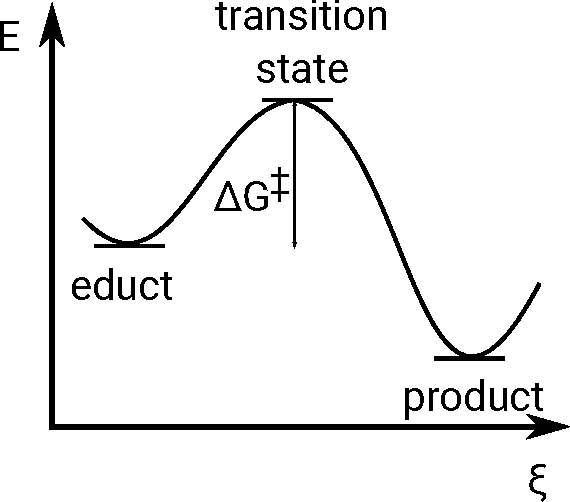
\includegraphics[width=0.4\textwidth]{figures/theory/MEP.pdf}
   \caption{Schematic view of a minimum energy path (MEP) for a thermal reaction. $\Delta$G$^\ddagger$ for the reaction is also plotted.}
            \label{abb:mep}
\end{figure}
\\
% One of the most prominent and widely used theories describing the transition state and the rate constants is Eyring theory of transition states. The most important approximations that are made are the following: i) there is an activated complex, ii) all particles that reached this complex/transition state will react towards the product. iii) At the transition state geometry, the motion along the reaction coordinate is seen as a one dimensional process and can be separated from all other degrees of freedom and can be seen as a translation.
% \\
% The equation for the rate constant is described by
% \begin{equation}\label{eyring}
% k(T)=\kappa\frac{k_BT}{h}e^{\Delta G^\ddagger(T)/(k_BT)},
% \end{equation}
% with the reaction rate constant $k$, Boltzmann's constant $K_B$, the temperature $T$, the difference of Gibb's free energy for the transition state and the educt $\Delta G^\ddagger$ and the transmission coefficient $\kappa$, that is a transmission coefficient (can be interpreted as a tunneling prefactor, for $\kappa>1$ tunneling occurs and for $\kappa<1$ non-classical reflection) \todo{tunneling corrections (seldomly applied in this work, not mention them here?)}, give the reaction rate constant as a function of temperature and barrier height. For the latter one needs to find the energies of the transition state and the educt. The educt geometry can simply be obtained by geometry optimization as a minimum on the PES.
% To find the transition state geometry and henceforth the energy we used Nudged Elastic Band calculations (NEB), with Climbing Image, Reaction path is approximated as a series of associated images, which are connected via spring forces. These spring forces prevent the images from optimizing into the local minimum next to the transition state. First a regular NEB, then on top of this climbing image was done which gives better convergence. In this calculation the energetically highest image is "optimized" towards higher energies in the contrary direction of the gradient.For the point found by this scheme we checked whether this is a transition state via frequency analysis, since a TST of first order has to have one imaginary mode, that vibrates along the reaction path.
Transition State Theory is a semi-classical theory: dynamics along the reaction coordinate $\xi$ are treated classically, but perpendicular directions allow for quantization of vibrational and rotational energy.
In thermodynamical equilibrium, all possible quantum states along the reaction coordinate are occupied  with respect to their Boltzmann weight $e^{\Delta E/(k_BT)}$.
\\
Assuming the reaction
\begin{equation}
A+ B \rightleftarrows C^\ddagger \rightarrow D
\end{equation}
where reactants $A$ and $B$ are in thermodynamical equilibrium with the transition state $C^\ddagger$ and this reacts to the product $D$.
The rate can then be determined with Eyring theory:
\begin{equation}\label{eq:eyring}
k(T)=\kappa\frac{k_BT}{h}e^{\Delta G^\ddagger(T)/(k_BT)}
\end{equation}
with the reaction rate constant $k(T)$, Boltzmann's constant $K_B$, the temperature $T$, the difference of Gibb's free energy for the transition state and the educt $\Delta G^\ddagger = \Delta G_{TS} - \Delta G_{educt}$, give the reaction rate constant as a function of temperature and free energy barrier height. Note, that this equation is only valid for cases, where all reactands that reach the TS react to the product site, \textit{i.e.} no re-crossing is employed, so the rate is in the classical picture the upper limit. For quantum effects, the rate can be increased due to tunneling, where reactants can overcome the barrier although they do not posses the sufficient amount of energy for the barrier. For this, the Eyring equation can be expanded with the transmission coefficient $\kappa$, that can be interpreted as a tunneling prefactor, for $\kappa>1$ tunneling occurs and for $\kappa<1$ non-classical reflection or re-crossing to the educt side.

For the barrier height one needs to find the energies of the transition state and the educt. The educt geometry can simply be obtained by geometry optimization as a minimum on the PES.
To find the transition state geometry and henceforth the energy we used Nudged Elastic Band calculations (NEB), with Climbing Image. The Reaction path is approximated as a series of associated images, which are connected via spring forces. These spring forces prevent the images from optimizing into the local minimum next to the transition state. First a regular NEB, then on top of this climbing image was done which gives better convergence. In this calculation the energetically highest image is "optimized" towards higher energies in the contrary direction of the gradient.For the point found by this scheme we checked whether this is a transition state via frequency analysis, since a TST of first order has to have one imaginary mode, that vibrates along the reaction path.

\section{From Density Functionals to Hybrids and Perturbation Theory}\label{theorybeyond}
\subsection{Hybrid Functionals}
In this work we also want to go beyond GGA (Generalized Gradient Approximation, here the PBE functional), because it is known from literature \cite{Zhao05} to underestimate reaction rates. Since we are interested in reaction kinetics it therefore is desirable to use more sophisticated methods to improve the rates. The first approach applied here is using hybrid functionals, where a fraction of exact exchange is mixed into the potential. For this the exchange correlation functional is split up into two parts:
\begin{equation}
 E_{xc}[n(\vec{r})]=  E_{x}[n(\vec{r})] + E_{c}[n(\vec{r})].
\end{equation}
The exchange part can be specified with a DFT part and HF with exact exchange:
\begin{equation}
 E_x = aE_x^{HF} + (1-a)E_x^{DFT}.
\end{equation}
with the parameter $a$, that gives the amount of exact Hartree-Fock exchange. As an example, the functional B3LYP consists of $20\%$ exact exchange.
\begin{equation}
 E_{xc}^{B3LYP}= aE_{xc}^{LDA} + (1-a)E_x^{HF} + bE_x^{B88} + cE_c^{LYP} + (1-c)E_c^{LDA}
\end{equation}
with $a=0.80$, $b=0.72$ and $c=0.81$.
\\
\subsection{M\o{}ller Plesset Peturbation Theory}
\todo{difference of MP2 to local MP2?}\\
Another ansatz is using Local M\o{}ller Plesset Peturbation Theory\cite{mollerplesset} of 2$^{\textrm{nd}}$ order (LMP2) as implemented in crystal/cryscor\todo{ citations}. These calculations are way more computationally demanding but offer better results on a higher level of theory. It offers more precise treatment of the dynamical electron correlation than DFT. The electronical Hamiltonian (here the subscript $e$ is omitted) has already been solved exactly or approximately. The solution to the given problem is similar to the already known one. The reference system $\hat{H}_0$ is perturbed by an external potential $\hat{V}$:
\begin{equation}
 \hat{H} = \hat{H}_0 + \lambda \hat{V}.
\end{equation}
$\hat{H}_0$ is the unperturbed Hamiltonian and $\lambda$ a parameter, that determines the extent of the perturbation, but in general it is considered as ``small'', compared to $\hat{H}_0$.
The perturbed Schr�dinger equation is given by:
\begin{equation}
 \hat{H}\Psi = E\Psi.
\end{equation}
If $\lambda=0$, $E=E^{(0)}$ and $\Psi=\Psi^{(0)}$ \todo{then what?}. For higher values of $\lambda$, the energy and the wave function change and can be written by expanding the ground state wave function $\Psi_0$ at $\lambda=0$
\begin{equation}
 \Psi_0 = \Psi_0^{(0)} + \lambda \Psi_0^{(1)} + \lambda^2\Psi_0^{(2)} + ...,
\end{equation}
the eigenvalues $E_0$ can be determined analogously as:
\begin{equation}
 E_0 = E_0^{(0)} + \lambda E_0^{(1)} + \lambda^2E_0^{(2)} + ...
\end{equation}
The superscript $E_0^{(n)}$ equals the correction of n-th level.\\
The unperturbed energy can be calculated with:
\begin{equation}
 E^{(0)} = <\Psi^{(0)}|\hat{H}^{(0)}|\Psi^{(0)}>=\sum\limits_{i=1}^N\varepsilon_i
\end{equation}
and the energy of $1^\textrm{st}$ order is:
\begin{equation}
 E^{(1)} = <\Psi^{(0)}|\hat{V}|\Psi^{(0)}>.
\end{equation}
$E^{(0)}+E^{(1)}$ equals the Hartree-Fock energy $E_{HF}$. For the energy of the second order, both occupied orbitals $i,j$ and unoccupied orbitals $k,l$ and their energy have to be considered:
\begin{equation}
 E^{(2)}=\sum\limits_{i}^{occ.}\sum\limits_{j>i}^{occ.}\sum\limits_{k}^{unocc.}\sum\limits_{l>k}^{unocc.} \frac{(<ij|kl> - <ij|lk>)^2}{\varepsilon_i + \varepsilon_j - \varepsilon_k - \varepsilon_l}
\end{equation}
The MP2-corrected total energy is composed of the HF energy and the second order energy:
\begin{equation}
 E_{MP2} = E^{(0)}+E^{(1)} + E^{(2)} = E_{HF} + E^{(2)}.
\end{equation}
The second order energy accounts for approximately $80-90\%$ of correlation which makes it a highly feasible method that includes electron correlation.
However, a main limitation of MP2 is the wave function of the zeroth order is a good approximation to the real system and the perturbation is rather small. If the wave function describes the system poorly, the corrections have to be higher and eventually, convergence is slow. In this case perturbation theory might not be a good option to describe correlation.

\section{Computational Details and Used Programs}
Vasp4.x, 5.2 and version x (newer), crystal, cryscor \todo{citations!}%, cp2k+i-pi, Turbomole
\\
For all the VASP calculations for the (0001) surface the parameters from prior work in our workgroup was used, like vacuum gap and convergence criteria, because these were converged carefully by Dr. Jonas Wirth\cite{WirthJPCC2012,Wirth2014,Wirth2015,Wirth2016}. Convergence was achieved when energies between two SCF steps was smaller then $10^{-5}\,$eV.
\\
For (11\=20) surface parameters were adopted and used as well. Also here the convergence criterion for the energy of two SCF cycles was $10^{-5}\,$eV.

For crystal and cryscor that were not used before for the calculation of alumina in our group the geometries from the VASP output were used as starting points and the usual convergence criteria of the programs were applied with some exception when convergence was hard to achieve.

\chapter{Water on $\upalpha$-Al$_2$O$_3$(11\=20)}
\section{Surface Model}
\todo{Fix Inconsistent figure references, don't always attach ", see figure X"}
\\
The structure of $\upalpha$-alumina has been well known for decades and was studied extensively (\textit{e.g.} \cite{Passerini1930,wyckoff1931}). It crystallizes in the hexagonal cell, that means $\uline{a}=\uline{b}\neq \uline{c}$, with an angle of $60$\textdegree{} between the cell vectors $\uline{a}$ and $\uline{b}$.
\\
To obtain the clean surface slab model of the (11\=20) surface a $2\times 2$ supercell was cut from the bulk. The corresponding cell vectors were adopted from the bulk structure and a vacuum gap in z-direction (perpendicular to the surface) was introduced to avoid unphysical interaction between the slabs in z-direction. In Figure \ref{abb:crystal_11-20}(a) apart from the (11\=20) surface the (0001) surface that is also studied in this work can be seen. Figure \ref{abb:crystal_11-20}(b) shows the top view and the cell vectors $\uline{a}$ and $\uline{b}$ of (11\=20). They are not equal to those in the hexagonal cell, but $\uline{a}=10.36$\AA, $\uline{b}=14.16$\AA~ and $\uline{c}=20.5$\AA. The angle $\theta$ between $\uline{a}$ and $\uline{b}$ is $84.56$\textdegree{} unlike the $60$\textdegree{} since the (11\=20) surface is tilted with respect to the top crystal plane. The nomenclature and color code of the surface Al and O atoms is also shown: The Alumina atoms have the same number of oxygen neighbor atoms but differ slightly in the arrangement of their neighbors and the distance in the relaxed structure, whereas the oxygen atoms in fact differ by the number of neighbors. In this work, the black spheres denote the CUSb atoms, the grey ones depict the CUSa. The twofold coordinated oxygen atoms (O-$\mu_2$) are shown in yellow and the threefold coordinated (O-$\mu_3$) in red. Atoms of the underlying layers are illustrated in pale colors, light grey for alumina and pale red for oxygen.
\begin{figure}[!h]
    \centering
    \subfigure[crystal]{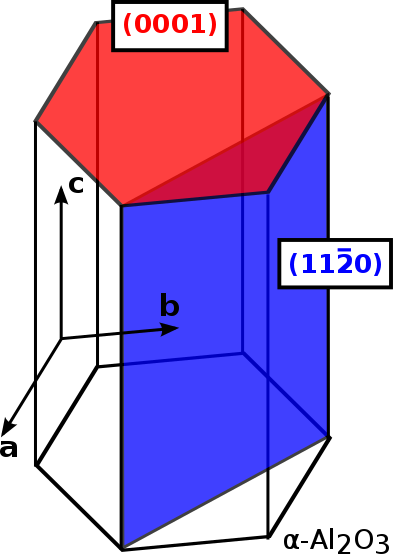
\includegraphics[width=0.30\textwidth]{figures/theory/al2o3-crystal.png}}
             \quad
             %add desired spacing between images, e. g. ~, \quad, \qquad, \hfill etc. (or a blank line to force the subfigure onto a new line)
    \subfigure[(11\=20), top view]{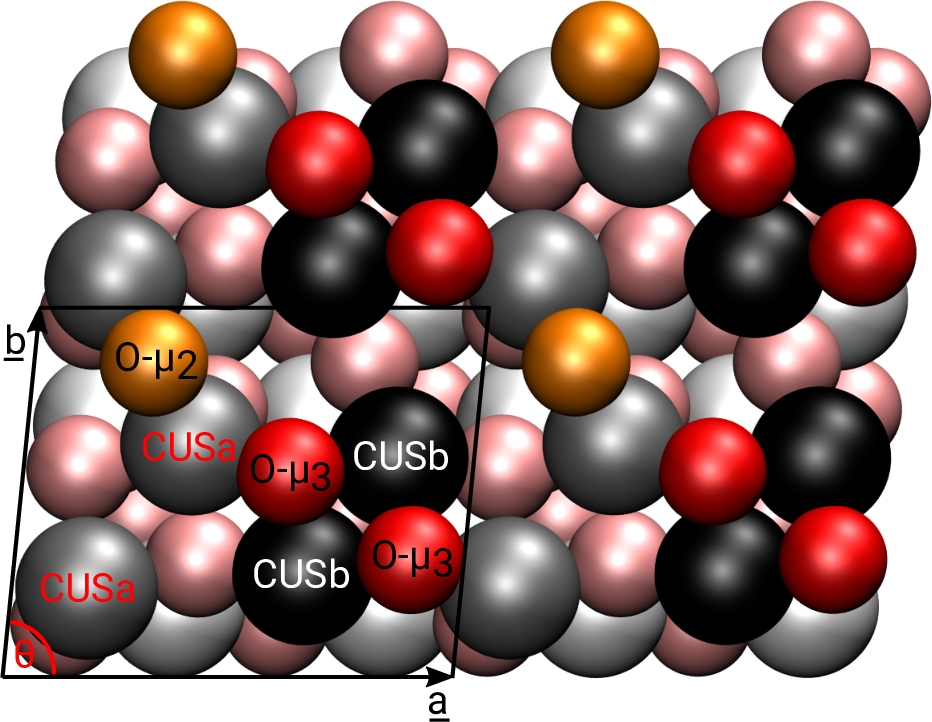
\includegraphics[width=0.30\textwidth]{figures/11-20/supercell_opt.png}}
             \quad
             %add desired spacing between images, e. g. ~, \quad, \qquad, \hfill etc. (or a blank line to force the subfigure onto a new line)
    \subfigure[(11\=20), side view]{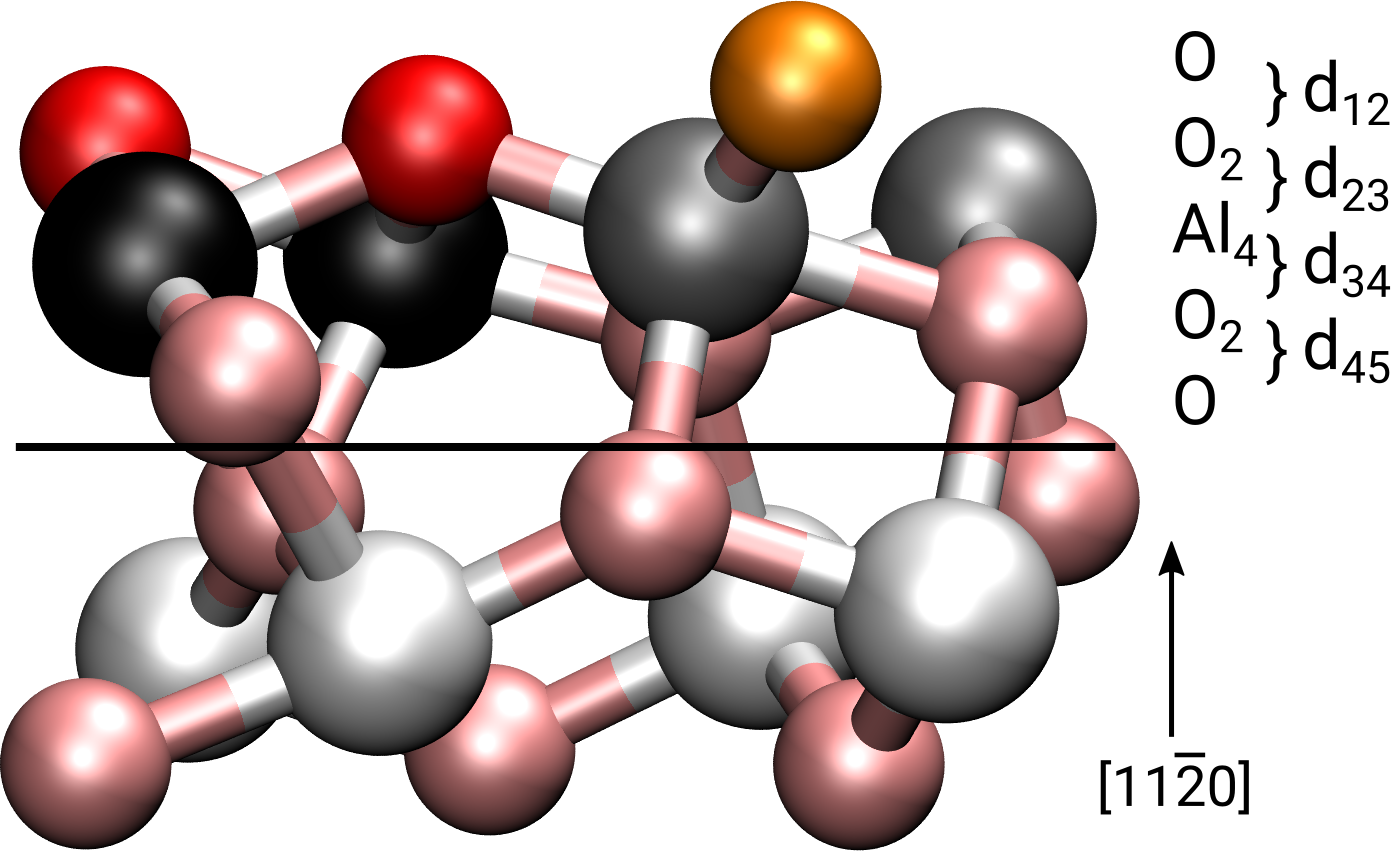
\includegraphics[width=0.30\textwidth]{figures/11-20/uc_opt.png}}
             \caption{The crystal cut of $\upalpha$-Al$_2$O$_3$, (a) schematic view compared to the (0001) surface, (b) a top view of the geometry optimized $2\times 2$ super cell with the nomenclature of the surface atoms. The two types of surface Al atoms (grey CUSa and black CUSb) as well as the twofold and threefold coordinated oxygen atoms (orange O-$\mu_2$ and red O-$\mu_3$). Subsurface atoms are indicated by pale colors. (c) gives the side view of the unit cell showing the distinctive atomic layers with the same color code.}
            \label{abb:crystal_11-20}
\end{figure}
\\
The unit cell consists of 5 atomic layers in z direction (O-O$_2$-Al$_4$-O$_2$-O), see Figure \ref{abb:crystal_11-20}(c)). The spacing between these layers in the relaxed structure and in the bulk crystal is slightly changed as given in Table \ref{tab:layer-dist}. A major issue of the optimization apart from layer spacing is that the interatomic distances of Al species change: the inter-CUSa\textendash inter-CUSa distance increased from $2.682$ to $2.994$\AA{}, the inter-CUSa\textendash CUSb distance increased from $2.833$ to $2.876$\AA{} whereas the CUSb\textendash CUSb distance decreased from $2.682$ to $2.499$\AA{}.
\\
The supercell that is mostly used in this work has 10 atomic layers, with the lowest 5 fixed to the bulk value to mimic the surface situation. For the calculation of the lattice vibrations up to 25 layers were considered (Figure \ref{abb:cell_sizes}). For each slab size the respective lowest 5 layers were kept fixed, see chapter \ref{phonons}. The spacing between the 5 top layers for each slab size is displayed in Table \ref{tab:layer-dist}.
\begin{table}[!ht]
  \centering
 \caption{Distances between the top 5 layers (see also numbering in Figure \ref{abb:crystal_11-20}(c)) for different optimized slab sizes and the unrelaxed bulk structure (right column). All values are given in \AA.} 
\vspace*{.2cm}
\begin{tabular}{c|cccc|c}
 &\multicolumn{4}{c}{total number of atomic layers} &\\
    distance    & 10   & 15   & 20   & 25   &bulk \\\hline
 d$_{12}$	&0.232 &0.234 &0.247 &0.245 &0.193 \\
 d$_{23}$	&0.642 &0.649 &0.638 &0.639 &0.741 \\
 d$_{34}$	&0.656 &0.655 &0.671 &0.672 &0.741 \\
 d$_{45}$	&0.198 &0.205 &0.209 &0.213 &0.191 \\
  \end{tabular}
  \label{tab:layer-dist}
\end{table}

\begin{figure}[!h]
    \centering
    \includegraphics[width=0.80\textwidth]{figures/11-20/cell_sizes.pdf}
             \caption{Side view for the different cell sizes for 10, 15, 20 and 25 layers in z-direction. Surface atoms are shown in the color code clarified before.}
            \label{abb:cell_sizes}
\end{figure}
$\vec{k}$-point tests were done for 5 different grid sizes from $1\times 1\times 1$ to $5\times 5\times 1$. In contrast to the even grid sizes, the odd ones contain the $\Gamma$-point and therefore are favorable. It can be deduced from Figure \ref{abb:11-20-kpointsampling} that the $3\times 3\times 1$ grid is already converged with respect to the energy of the clean surface.
\begin{figure}[!h]
\centering
 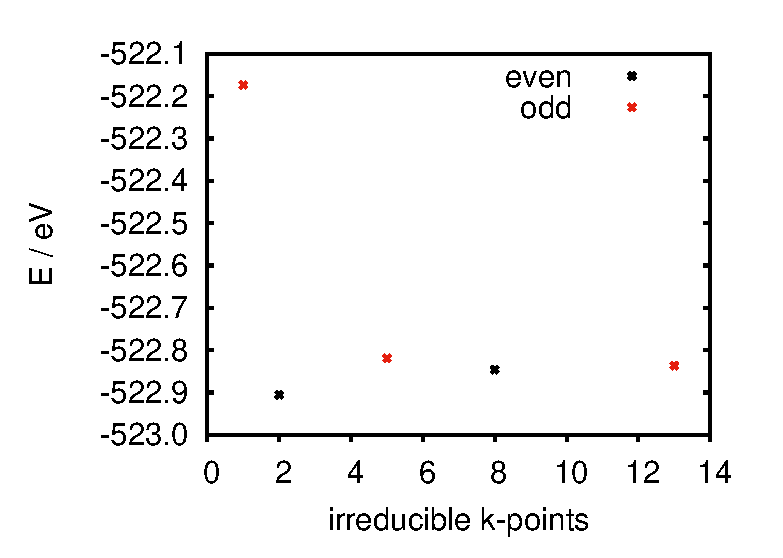
\includegraphics[width=0.4\textwidth]{figures/11-20/irreducibles-E.eps}
   \caption{Sampling of the $\vec{k}$-points, shown is the energy of the optimized super cell with respect to the number of irreducible $\vec{k}$-points. The even values correspond to the $2\times 2 \times 1$ (2 irreducibles) and $4\times 4\times 1$ (8 irr.), whereas the odd, which contain the $\Gamma$-point, are described by $1\times 1\times 1$ (1 irr.), $3\times 3\times 1$ (5 irr.) and $5\times 5\times 1$ (13 irr.).}
            \label{abb:11-20-kpointsampling}
\end{figure}
\\
Starting from the $2\times 2$ supercell approach of the clean surface there are 16 CUS Al-atoms (Coordinatively Unsaturated Sites). These have fewer bonds than the aluminum atoms in the bulk structure since the surface layer is  depleted. These atoms are very interesting for adsorbate molecules/atoms, because these surface atoms are electron rich and can be addressed for adsorption. Theoretically, these 16 atoms could be covered with adsorbates (in this work water) to gain 1 mono layer (ML). As will be shown shortly, water can not adsorb on all 16 Al CUS simultaneously to get 1ML. Of these 16 CUS atoms eight are CUSa and eight CUSb. On top of CUSb, a water molecule/OH residue can adsorb, but on top of a CUSa the adsorbate roams to an bridging inter-CUSa position between two CUSa. Due to this the number of potential adsorbates is decreased to 12.

\section{Structure Search}\label{structure_search11-20}
To study water adsorption, first a low coverage regime was investigated: 1 water molecule per $2\times 2$ supercell, which equals a coverage of 1/12. The procedure was the following: put molecular water at different positions on the surface and let it relax. By doing this one molecular minimum and several dissociated species including both CUS and oxygen types were found. This multitude of different surface atoms gives rise to a large variety of possible adsorption geometries. Adsorption energies and Gibb's free energy of the resulting next neighbor species can be seen in Table \ref{tab:ads_1water}. The nomenclature for the adsorption sites that is used in the following gives at first the type of Al site where the OH-residue (/OH$^-$) is adsorbed and at second place the oxygen type where the H(/H$^+$) is adsorbed (OH-site$\parallel$H-site). The term "inter" that is used in the following characterizes a position between two CUS atoms and leads to a bidentate adsorption pattern. The additional notation with $^\prime$ denotes greater distances between the residues. There is also one metastable molecular species that appears to be more stable than the found molecular minimum considering adsorption energy, but it cannot be classified as a stable minimum since there is one imaginary mode displaying the movement of the proton towards the dissociated species.
\\
The adsorption energy is defined by Equation \ref{eq:Eads} as the energy of the adsorbed system compared to the energies of the clean surface and the isolated water molecule:
\begin{equation}\label{eq:Eads}
 E_\textrm{ads}=E_\text{ads. species}-(E_\text{free water molecule}+E_\text{surface}).
\end{equation}

\begin{table}[!ht]
  \centering
 \caption{For molecular and (singly) dissociated water on $\upalpha$-Al$_2$O$_3$(11\=20) adsorption energies E$_\textrm{ads}$ and Gibb's free energy $G_\textrm{ads}$ for different temperatures are given in eV. E$_\textrm{ads}$ was calculated from Equation \ref{eq:Eads} and G$_\textrm{ads}$ is defined analogously. These results were obtained with PBE+D2. The three most stable configurations are marked with bold letters.
\vspace*{.2cm} 
  }
  \begin{tabular}{cl|cccc}
   \multicolumn{2}{c|}{Adsorbed Species}  & $E_\text{ads}$ & $G_\text{ads, 130 K}$  &  $G_\text{ads, 300 K}$  & $G_\text{ads, 400 K}$ \\
\hline
\multirow{1}{*}{molecular} & CUSb          &   -1.78  &-1.60 & -1.51  & -1.46 \\
  \hline
 \multirow{6}{*}{dissociated} & \textbf{inter-CUSa||O-$\mu_2$} & \textbf{-2.50} &-2.27 & -2.16 & -2.09 \\
  & inter-CUSa||O-$\mu_3$ & -1.67 &-1.44 &-1.33 & -1.27 \\
  & \textbf{CUSb||O-$\mu_2$} & \textbf{-2.28} & -2.12& -2.03 &-1.97  \\
 & CUSb||O-$\mu_3$ & -1.19 &-1.05 &-0.98 & -0.95 \\%Cb3_other
 & \textbf{inter-CUSb||O-$\mu_2$} & \textbf{-2.09} &-1.88 &-1.80 & -1.76 \\
 & inter-CUSb||O-$\mu_3$ & -1.89 &-1.71 & -1.63 & -1.58 \\
  \end{tabular}
  \label{tab:ads_1water}
\end{table}
\begin{figure}[!ht]
 \centering
\subfigure[CUSb]{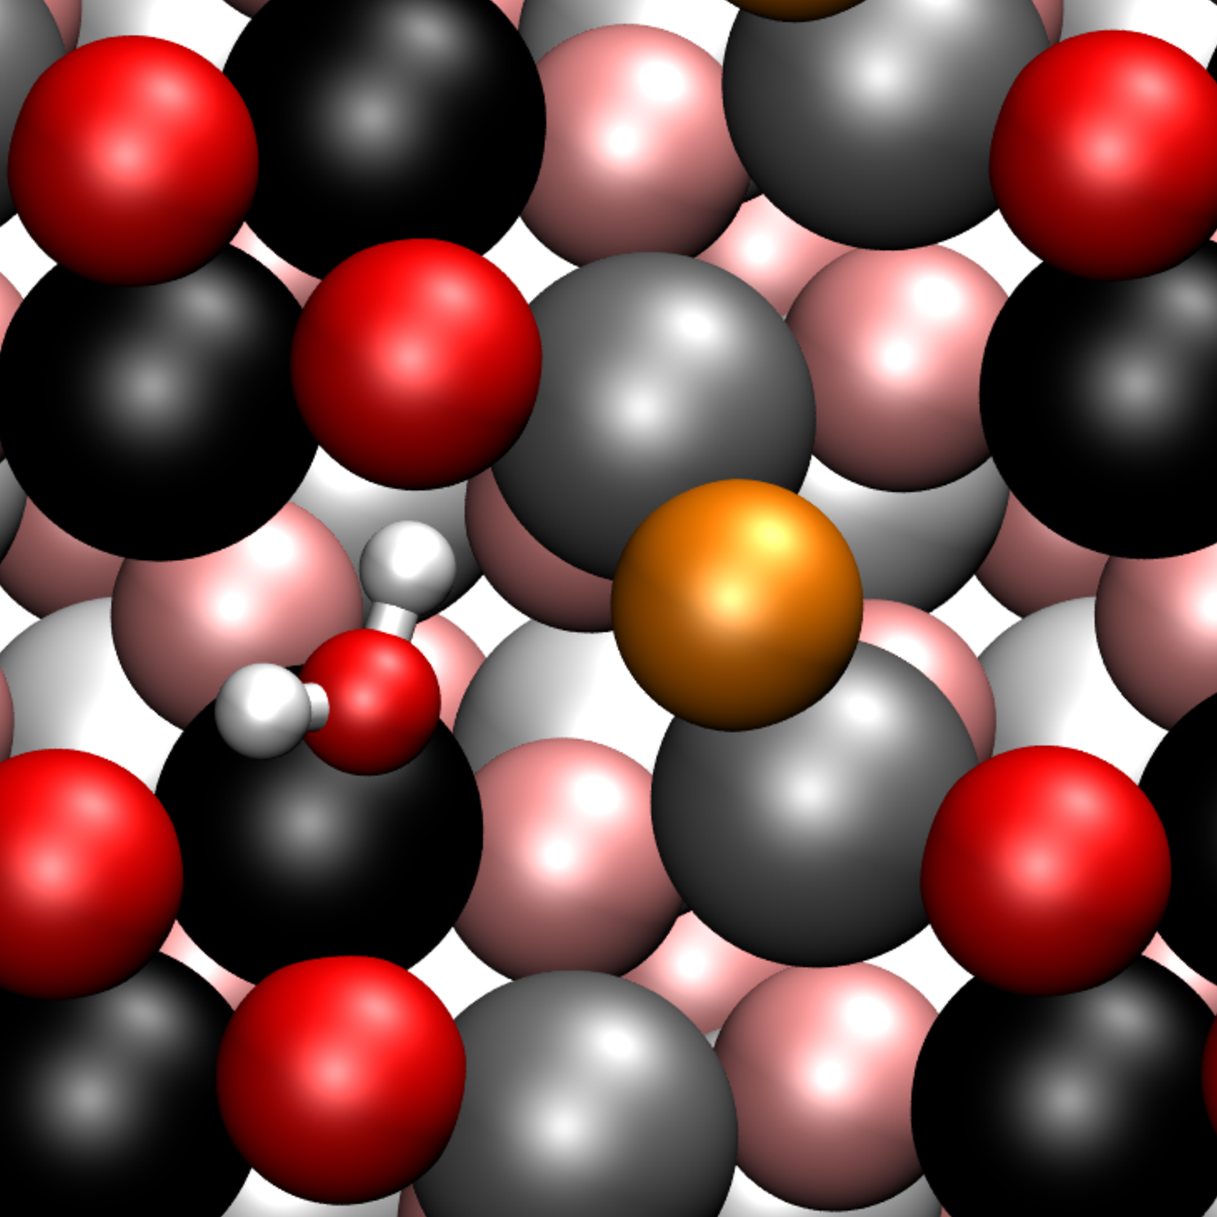
\includegraphics[width=0.2\textwidth]{figures/11-20/test-Cb.pdf}}
 \quad\quad
 \subfigure[inter-CUSa||O-$\mu_2$]{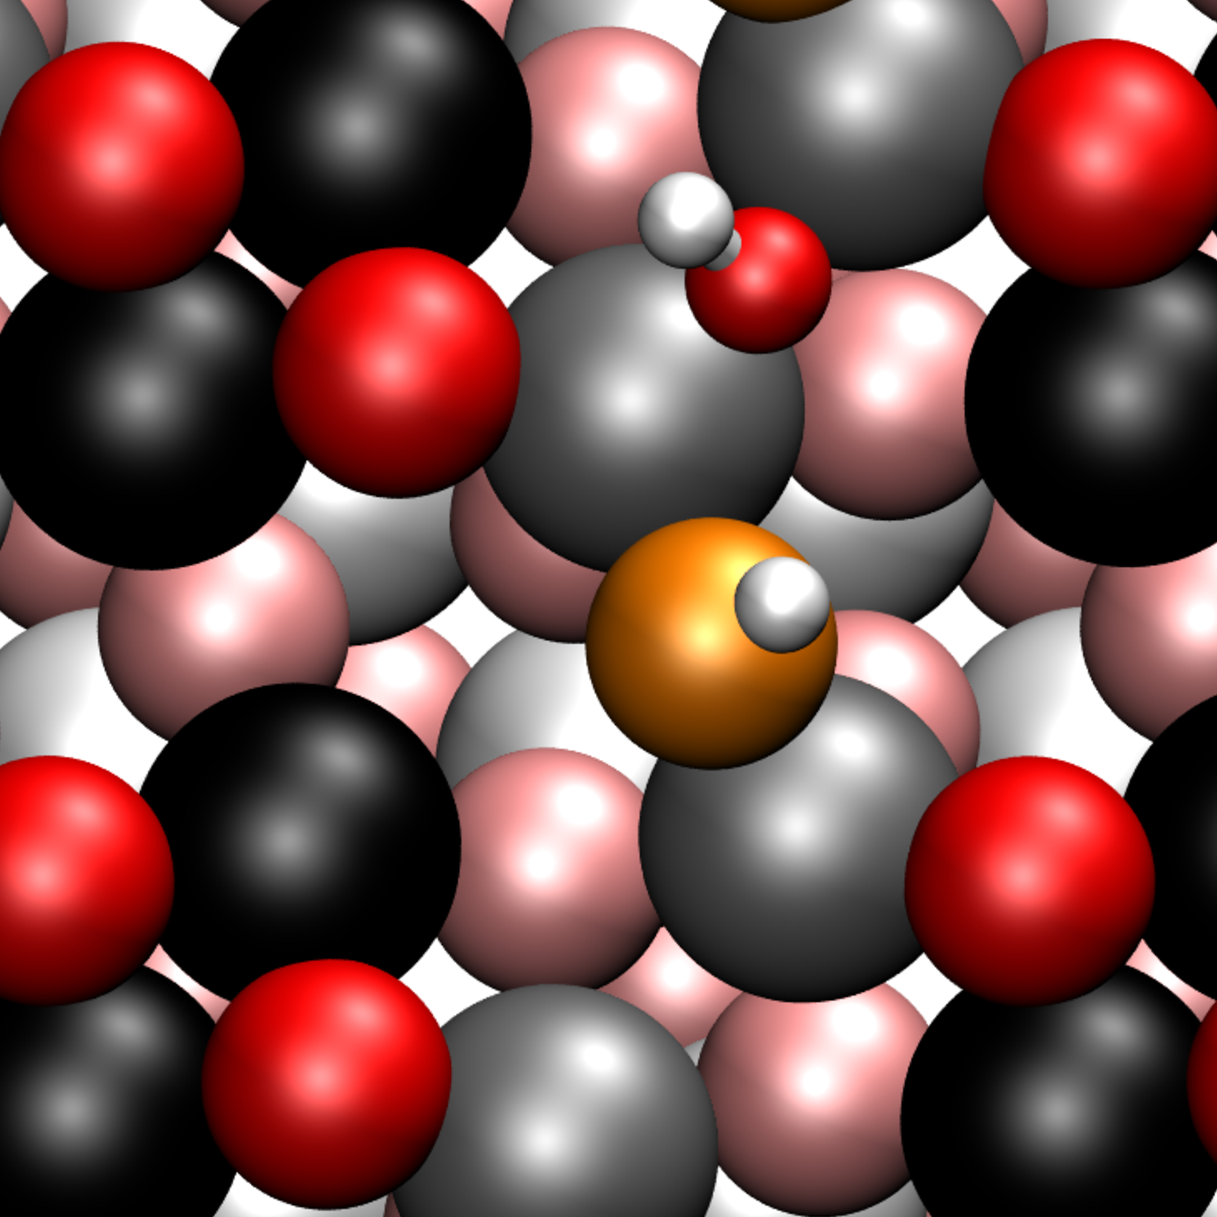
\includegraphics[width=0.2\textwidth]{figures/11-20/test-iCa2.pdf}}
  \quad
\subfigure[CUSb||O-$\mu_2$]{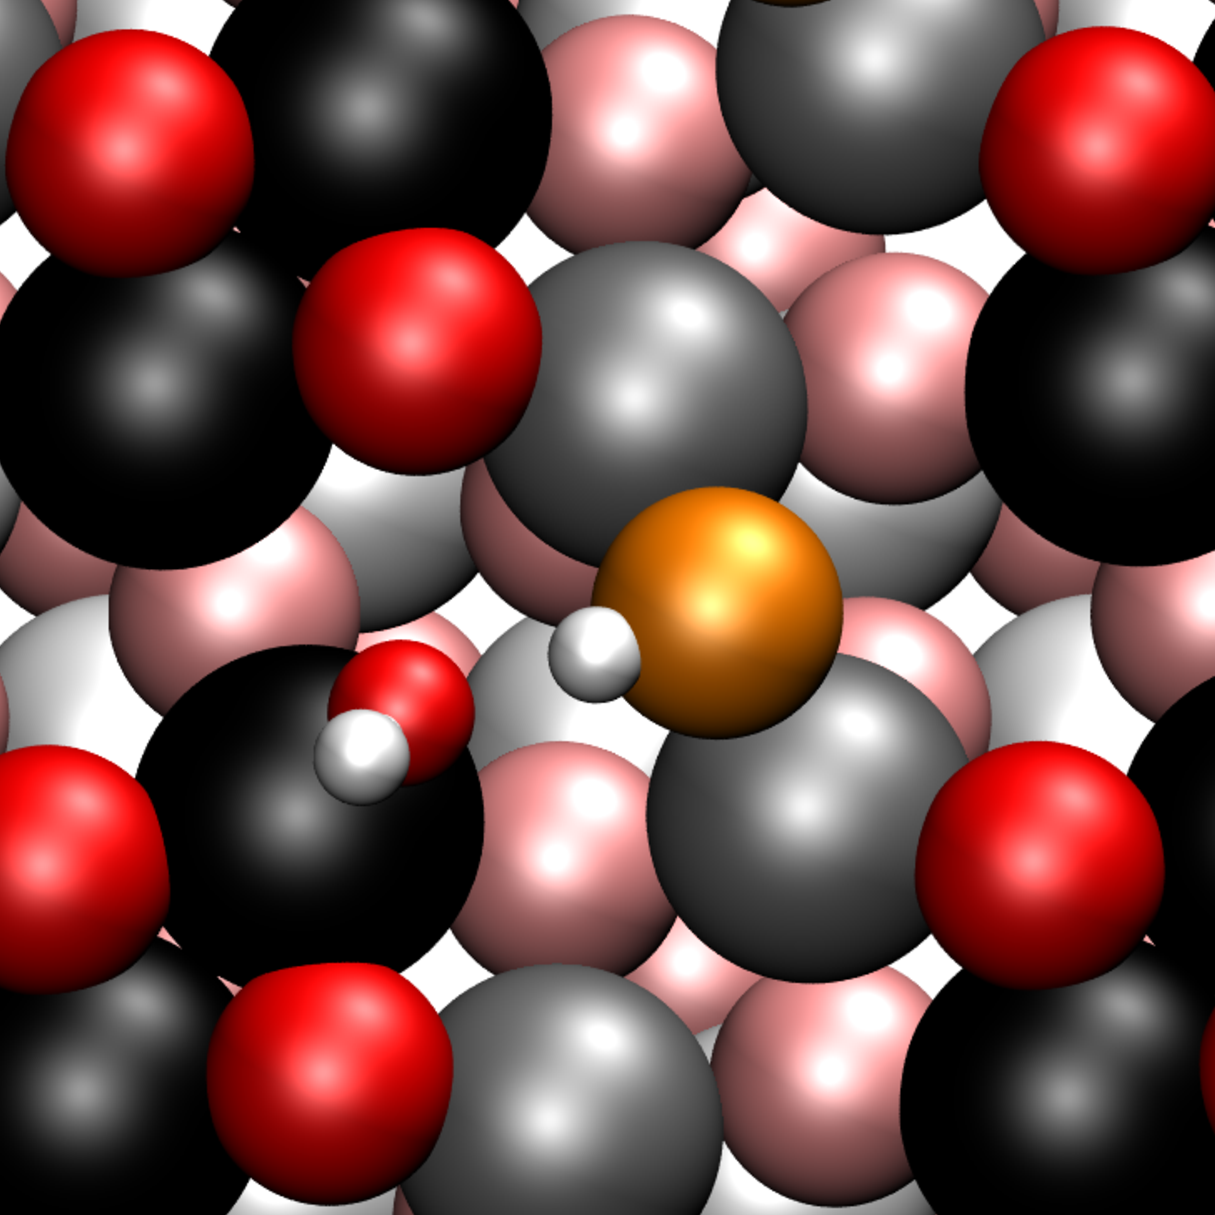
\includegraphics[width=0.2\textwidth]{figures/11-20/test-Cb2.pdf}}
 \quad
\subfigure[inter-CUSb||O-$\mu_2$]{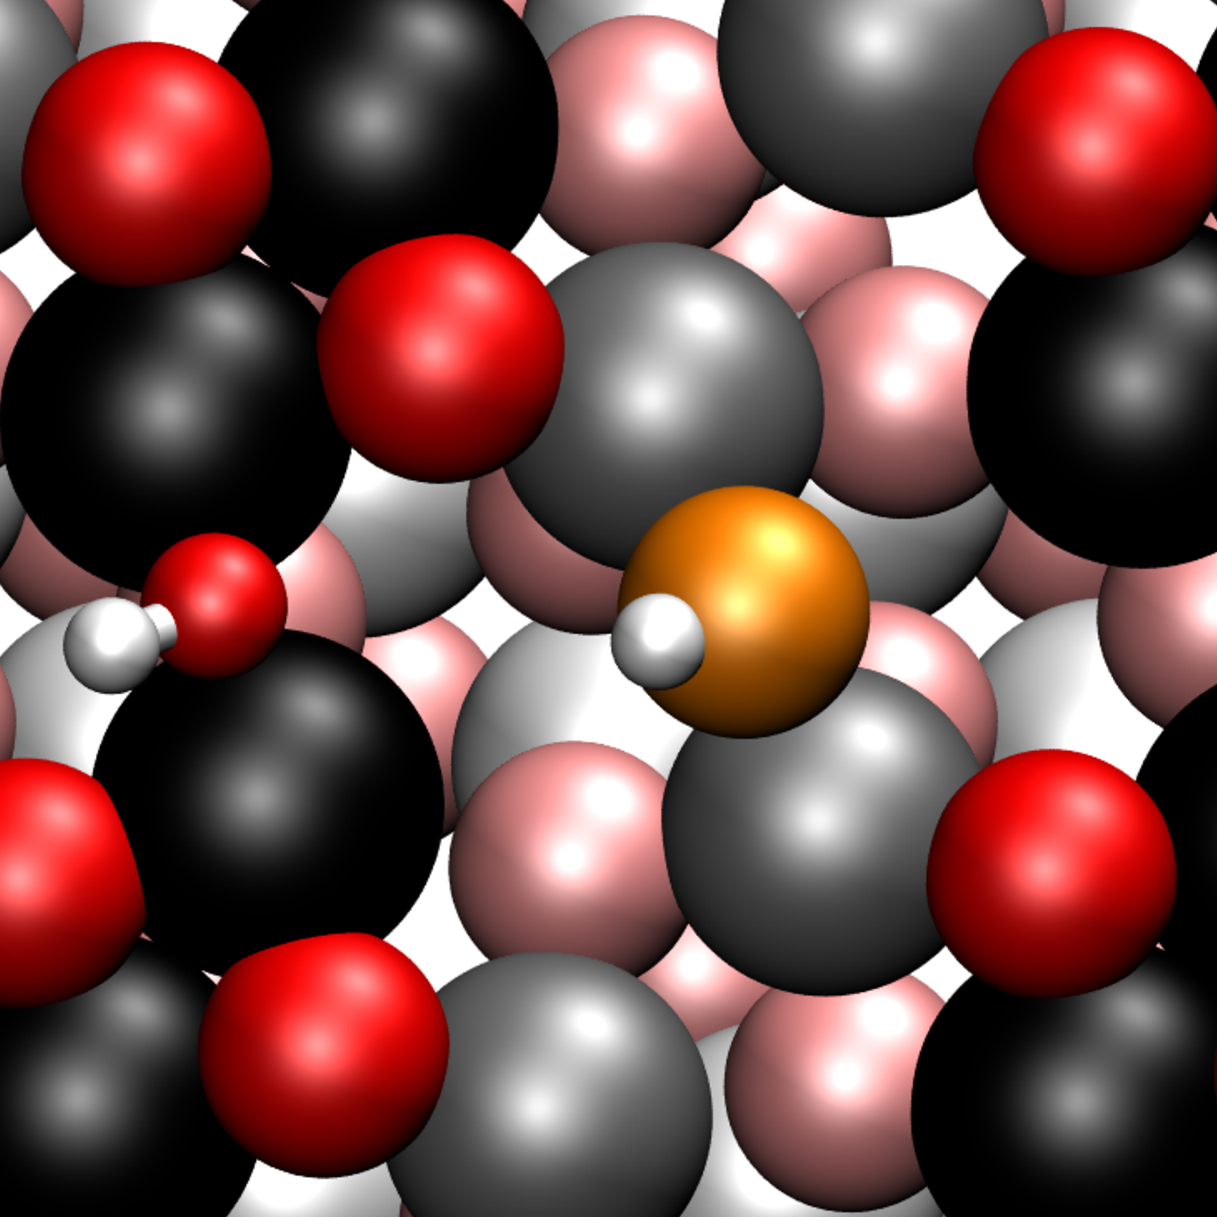
\includegraphics[width=0.2\textwidth]{figures/11-20/test-iCb2.pdf}}
\quad
\subfigure[inter-CUSa||O-$\mu_3$]{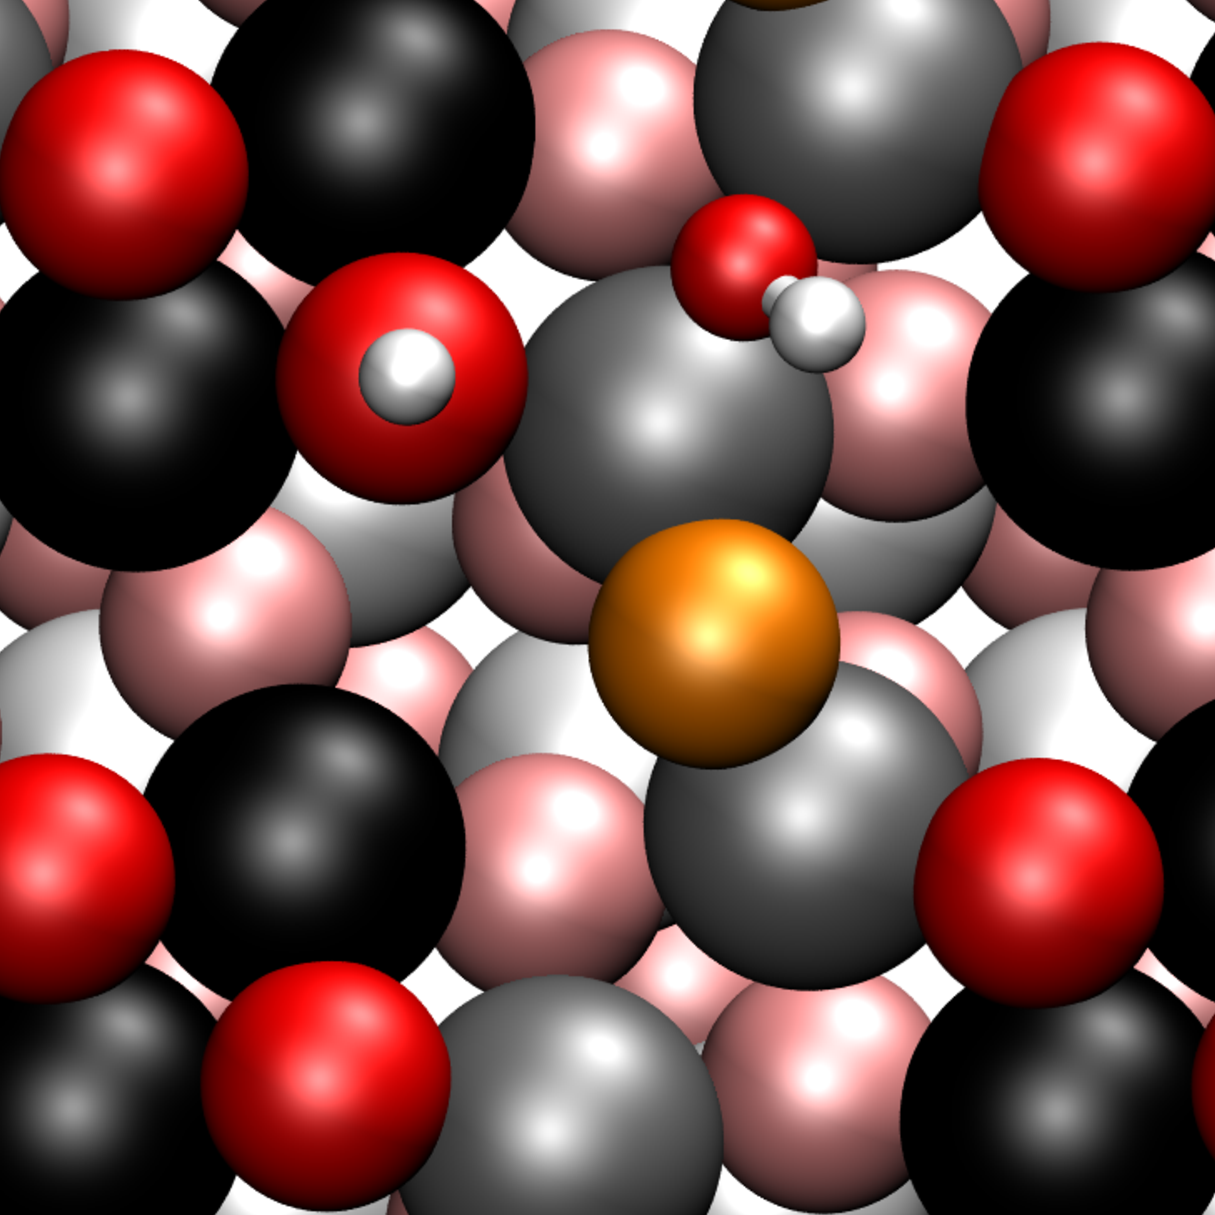
\includegraphics[width=0.2\textwidth]{figures/11-20/test-iCa3.pdf}}
 \quad
\subfigure[CUSb||O-$\mu_3$]{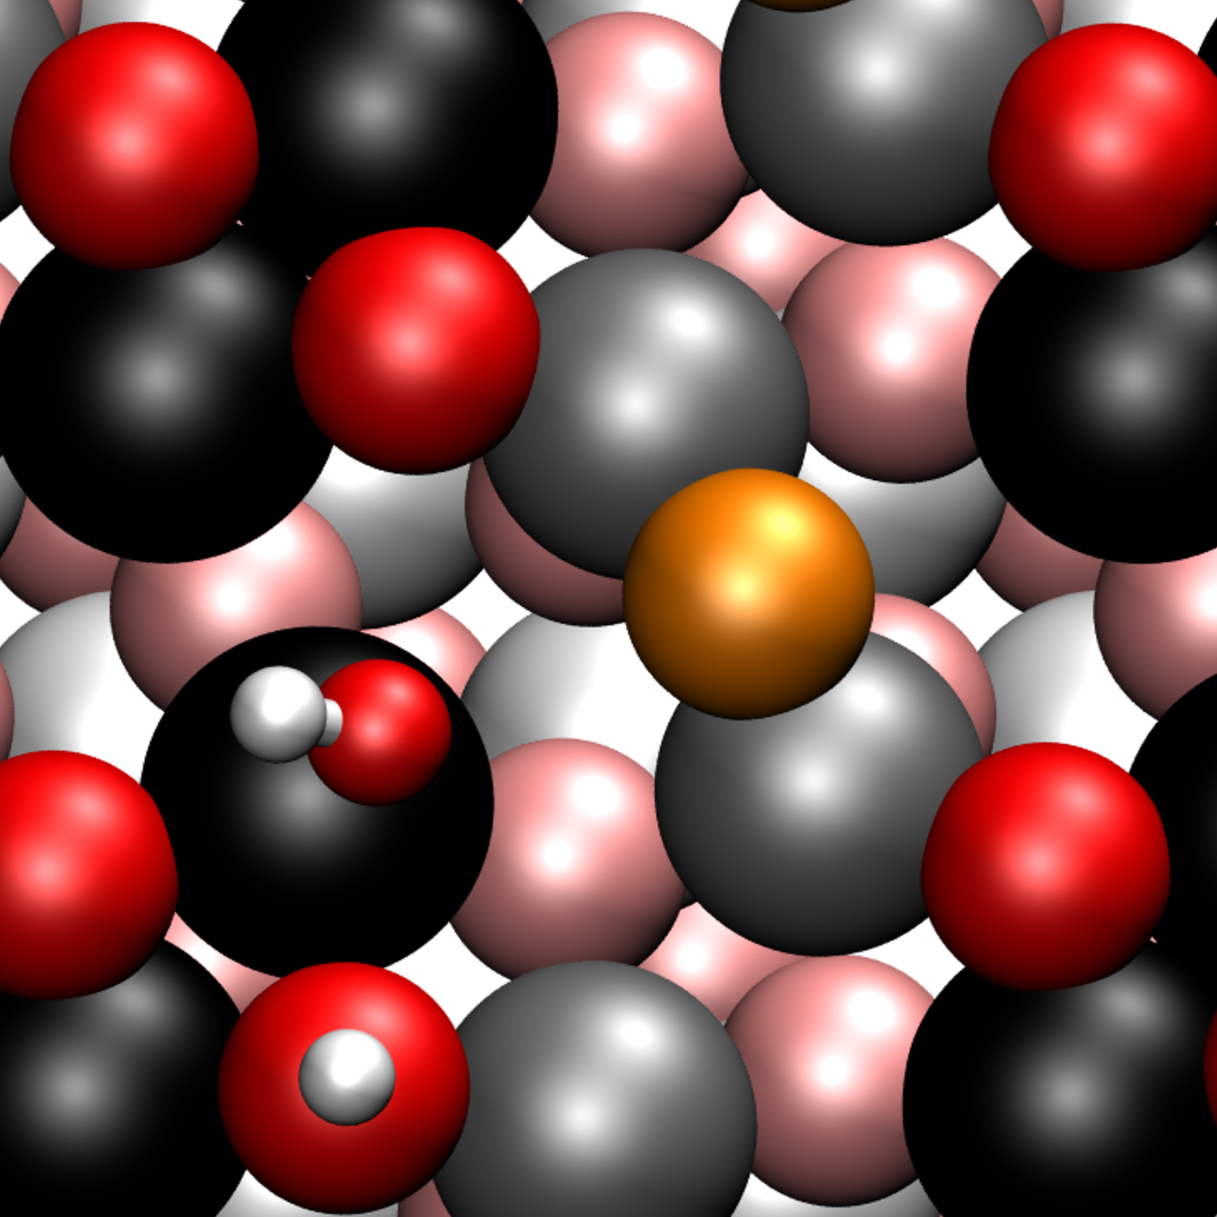
\includegraphics[width=0.2\textwidth]{figures/11-20/test-Cb3.pdf}}
 \quad
\subfigure[inter-CUSb||O-$\mu_3$]{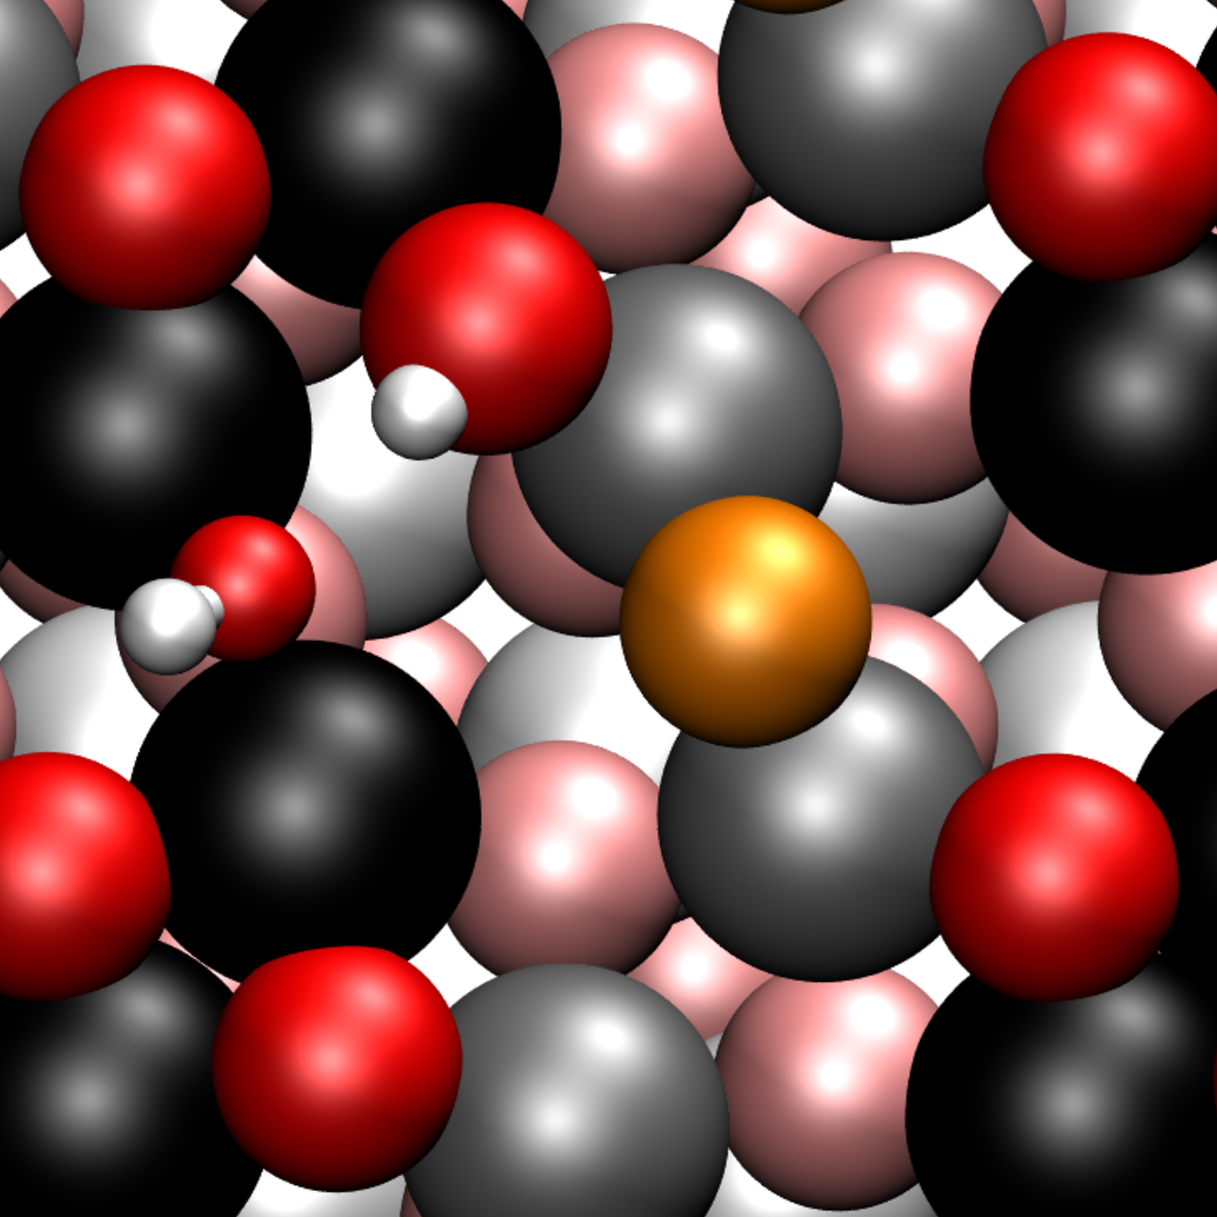
\includegraphics[width=0.2\textwidth]{figures/11-20/test-iCb3.pdf}}
 \caption{Top view of the adsorption geometries for molecular CUSb (a) and the next neighbor dissociated water 
((b)-(g)). The color code is the same as in Figure \ref{abb:crystal_11-20}(b) and (c), CUSa grey, CUSb black, O-$\mu_2$ yellow and O-$\mu_3$ red; Hydrogen is illustrated in white; subsurface layers are shown in pale colors.}
        \label{abb:ads-geoms}
 \end{figure}

The molecular minimum is substantially less stable than the dissociated species. On the contrary, the dissociated water is very stable, even in comparison to the more stable surface cuts (0001) and (1\=102) that were previously investigated in our group by Dr. Jonas Wirth\cite{Wirth2016,WirthJPCC2012}. Dissociated species, where the proton is located at a twofold coordinated surface oxygen are far more stable than the corresponding systems where the threefold coordinated is occupied. This is due to the higher negative charge and the higher basicity of such a twofolded oxygen atom in comparison with the more saturated threefold coordinated O-$\mu_3$ oxygen atom. In fact, the adsorption can be seen as a Lewis acid / base reaction\cite{Stair1981} with the Lewis acid character of the undercoordinated aluminum and the base character of the oxygen from the water molecule.
\\
The adsorption of OH at an inter-CUSa site is more favorable than at a CUSb site, because the former corresponds to a site where in the bulk system another oxygen atom would be situated, which is not the case for the CUSb position. Additionally, the CUSb position is electronically and sterically more hindered because of the two threefold coordinated oxygen atoms in the surroundings.
\\
Dissociated species in direct neighborhood as shown in Table \ref{tab:ads_1water} and Figure \ref{abb:ads-geoms} are more stable than those where the proton and the OH residue are further apart (see Table \ref{tab:ads_1waterfurther}), because the OH residue has a stabilizing effect on the H. It is apparent from this table that the inter-CUSb||O-$\mu_3^{\prime\prime\prime}$-species is more stable than the species inter-CUSb||O-$\mu_3^{\prime\prime}$. This is due to the fact that the periodic conditions actually lead to a decrease of the distance between OH groups in the former system. The distances between the neighboring OH groups in the O-$\mu_3^{\prime\prime}$ system are $6.19$ and $8.82\,$\AA{}, compared to $6.64$ and $8.96\,$\AA{} in the O-$\mu_3^{\prime\prime\prime}$ system (the numbers refer to the two possible distance in the periodic system, direct and over the border of the unit cell). The latter one is in fact only slightly further away, the average distance is $0.739$\AA{} for inter-CUSb$\parallel$O-$\mu_3^{\prime\prime}$ and $0.780$\AA{} for inter-CUSb$\parallel$O-$\mu_3^{\prime\prime\prime}$. Although the distance is larger, there seems to be more stabilization\todo{mysterious..}. For examples of the corresponding  diffusion reactions, see chapter \ref{reactions}.
\begin{table}[!ht]
  \centering
 \caption{Comparison of adsorption energies for next neighbor dissociated species and dissociated species where OH and H are further apart. Results are given in eV.
\vspace*{.2cm} 
  }
  \begin{tabular}{cc}
  Adsorbed Species  & $E_\text{ads}$  \\
   inter-CUSa||O-$\mu_3$ & -1.67 \\
   inter-CUSa||O-$\mu_3^\prime$ & -1.42 \\\hline
   inter-CUSb||O-$\mu_3$ & -1.89\\
   inter-CUSb||O-$\mu_3^{\prime\prime}$ & -1.16\\
   inter-CUSb||O-$\mu_3^{\prime\prime\prime}$ & -1.22\\
  \end{tabular}
  \label{tab:ads_1waterfurther}
\end{table}
\\
Apart from that, systems with additional atomic layers were studied to gain knowledge towards more realistic systems. The corresponding adsorption energies are shown in Table \ref{tab:eads_layers}. Basically, the findings do not differ largely with increasing slab size. The molecular species still is less stable than the O-$\mu_2$ dissociated species and is more stable than the O-$\mu_3$ dissociated ones (except for inter-CUSb$\parallel$O-$\mu_3$ dissociated system). inter-CUSa$\parallel$O-$\mu_2$ is the most stable structure through all sampled systems sizes, inter-CUSb$\parallel$O-$\mu_2$ and CUSb$\parallel$O-$\mu_2$ change their stability (it approaches to nearly the same value for 25 layers) depending on the number of layers but still are some orders of magnitude less probable than inter-CUSa$\parallel$O-$\mu_2$. Dissociated systems occupying the threefold coordinated surface oxygen atom remain in the same stability order.
%For higher quantity of layers, the inter-CUSb gets more favourable than CUSb, both for O-$\mu_2$ and O-$\mu_3$. This might be due to less interaction between neighboring oxygen atoms with the inter-CUSb adsorbed OH group.
  \begin{table}[!ht]
  \centering
  \caption{Adsorption energies calculated from equation \ref{eq:Eads} for molecular and dissociated species for different vertical slab sizes. All values are given in eV. The most stable systems (inter-CUSa$\parallel$O-$\mu_2$, CUSb$\parallel$O-$\mu_2$ and inter-CUSb$\parallel$O-$\mu_2$ are highlighted in bold letters.}
 \begin{tabular}{l|cccc}
 System                     & 10 layers& 15 layers& 20 layers&  25 layers \\\hline
CUSb                                    &-1.78 &-1.80     &-1.81     &-1.83      \\\hline
\textbf{inter-CUSa$\parallel$O-$\mu_2$}    &\textbf{-2.50} &\textbf{-2.4}6 &\textbf{-2.54} &\textbf{-2.56}  \\
inter-CUSa$\parallel$O-$\mu_3$          &-1.67 &-1.67 &-1.78 &-1.80 \\
\textbf{CUSb$\parallel$O-$\mu_2$}          &\textbf{-2.28} &\textbf{-2.35} &\textbf{-2.36} &\textbf{-2.35} \\
CUSb$\parallel$O-$\mu_3$                &-1.19 &-1.71 &-     &-      \\
\textbf{inter-CUSb$\parallel$O-$\mu_2$}    &\textbf{-2.09} &\textbf{-2.43} &\textbf{-2.48} &\textbf{-2.36}  \\
inter-CUSb$\parallel$O-$\mu_3$          &-1.89 &-1.59 &-1.65 &-2.09 
\label{tab:eads_layers}
\end{tabular}
 \end{table}
\\
Table \ref{tab:eads_layers} shows that the most stable systems are already converged for the 10-layer slab with regard to adsorption energies (and also vibrational OH/OD frequencies as will be seen in section \ref{nma}).
\\
Furthermore, systems with a higher water coverage were considered to model enhanced systems, some cases for 2 water molecules ($16.6\%$ coverage), 4 inter-CUSa$\parallel$O-$\mu_2$ ($33.3\%$ coverage) and a fully covered supercell (12 moleculas, $100\%$), for these systems normal mode analyses were carried out to get vibrational spectra, see chapter \ref{phonons}. Structures can be found in Figures \ref{abb:2water} and \ref{abb:4+fully}.
\begin{figure}[!ht]
 \centering
\subfigure[CUSb+CUSb$\parallel$O-$\mu_2$]{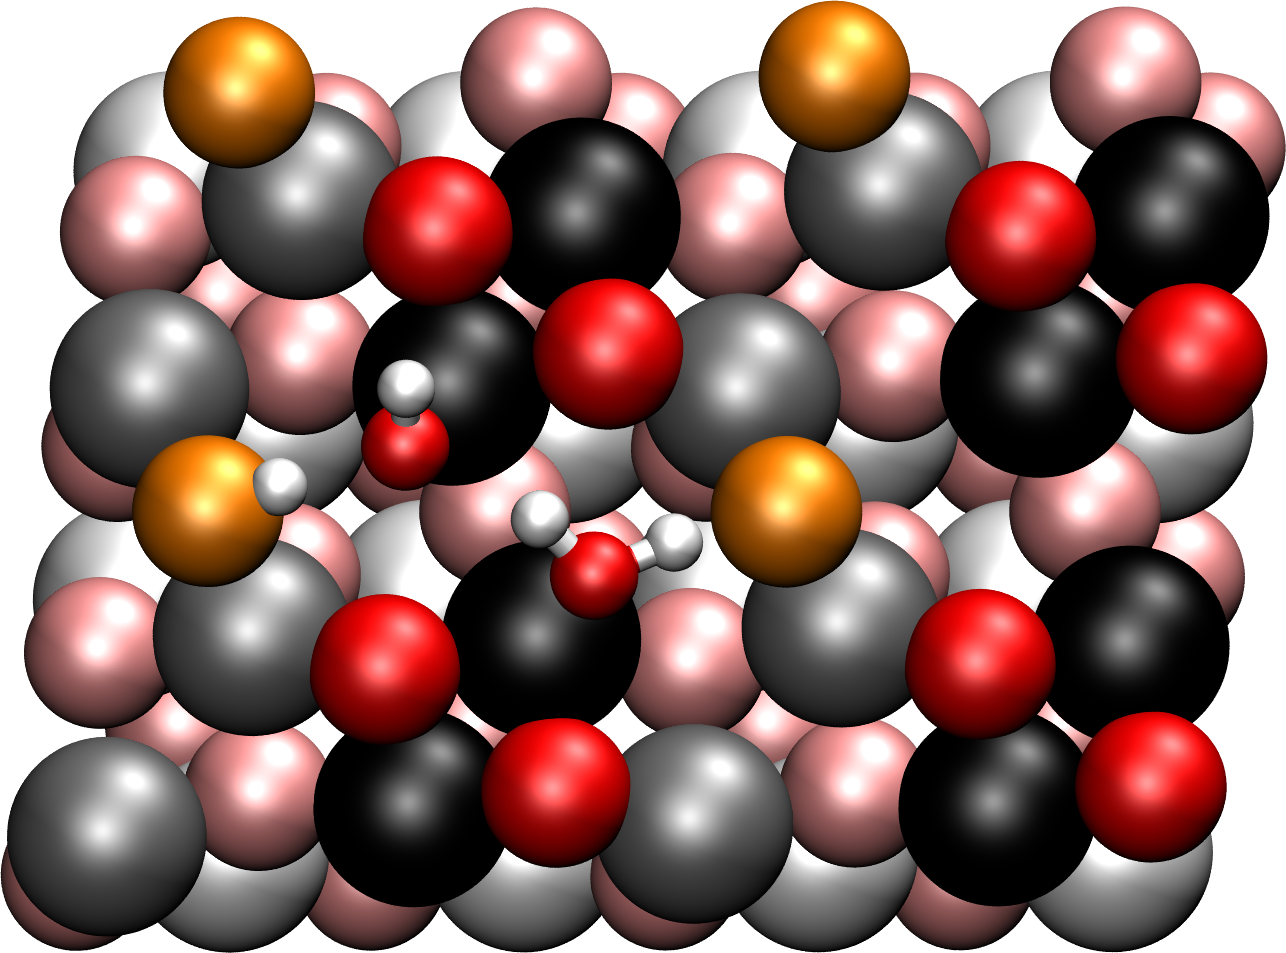
\includegraphics[width=0.302\textwidth]{figures/11-20/Cb-Cb2.png}}
 \quad\quad
 \subfigure[inter-CUSa||O-$\mu_2$+CUSb$\parallel$O-$\mu_2$]{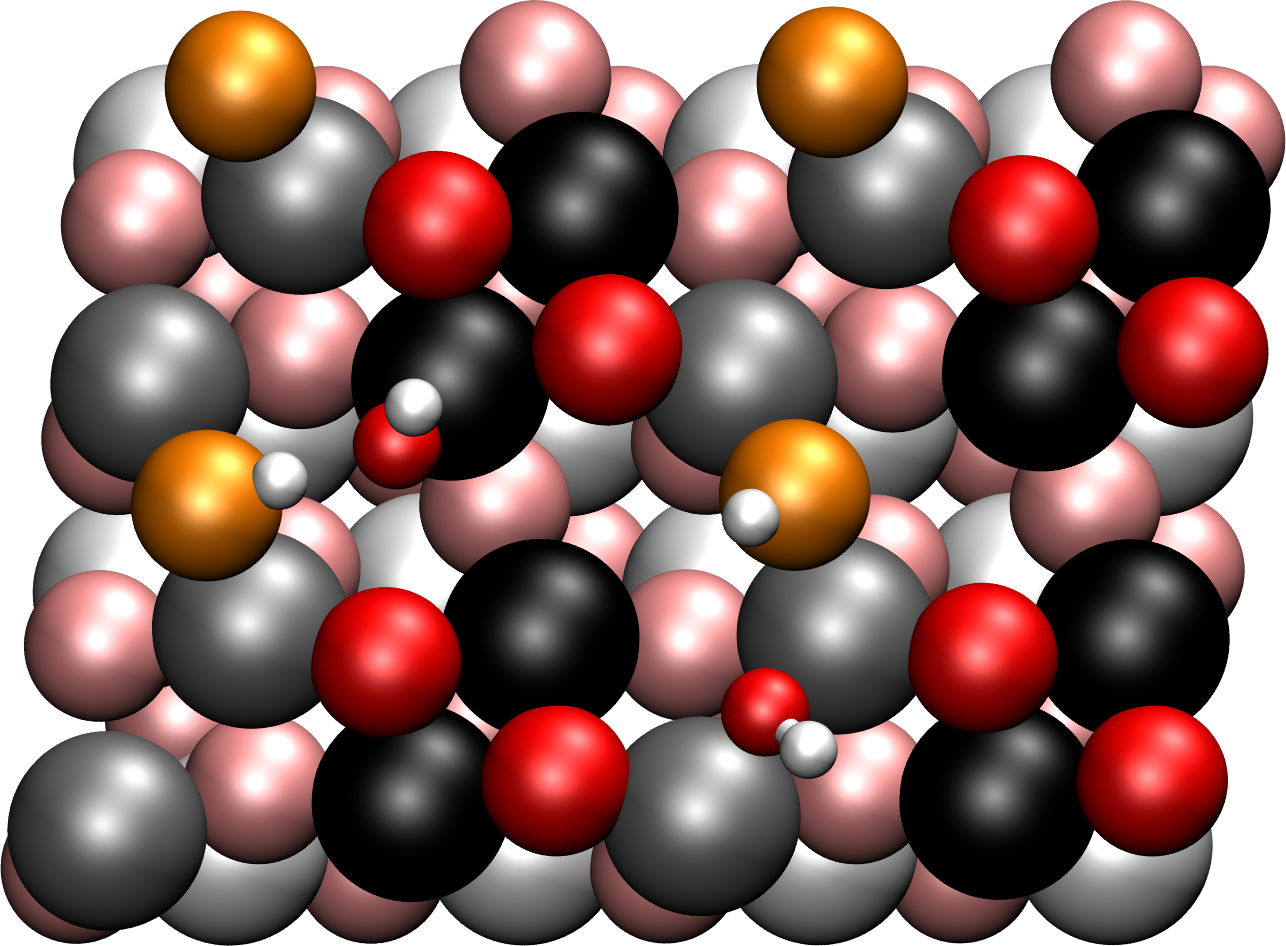
\includegraphics[width=0.304\textwidth]{figures/11-20/iCa2-Cb2.png}}
  \quad
\subfigure[2inter-CUSa||O-$\mu_2$]{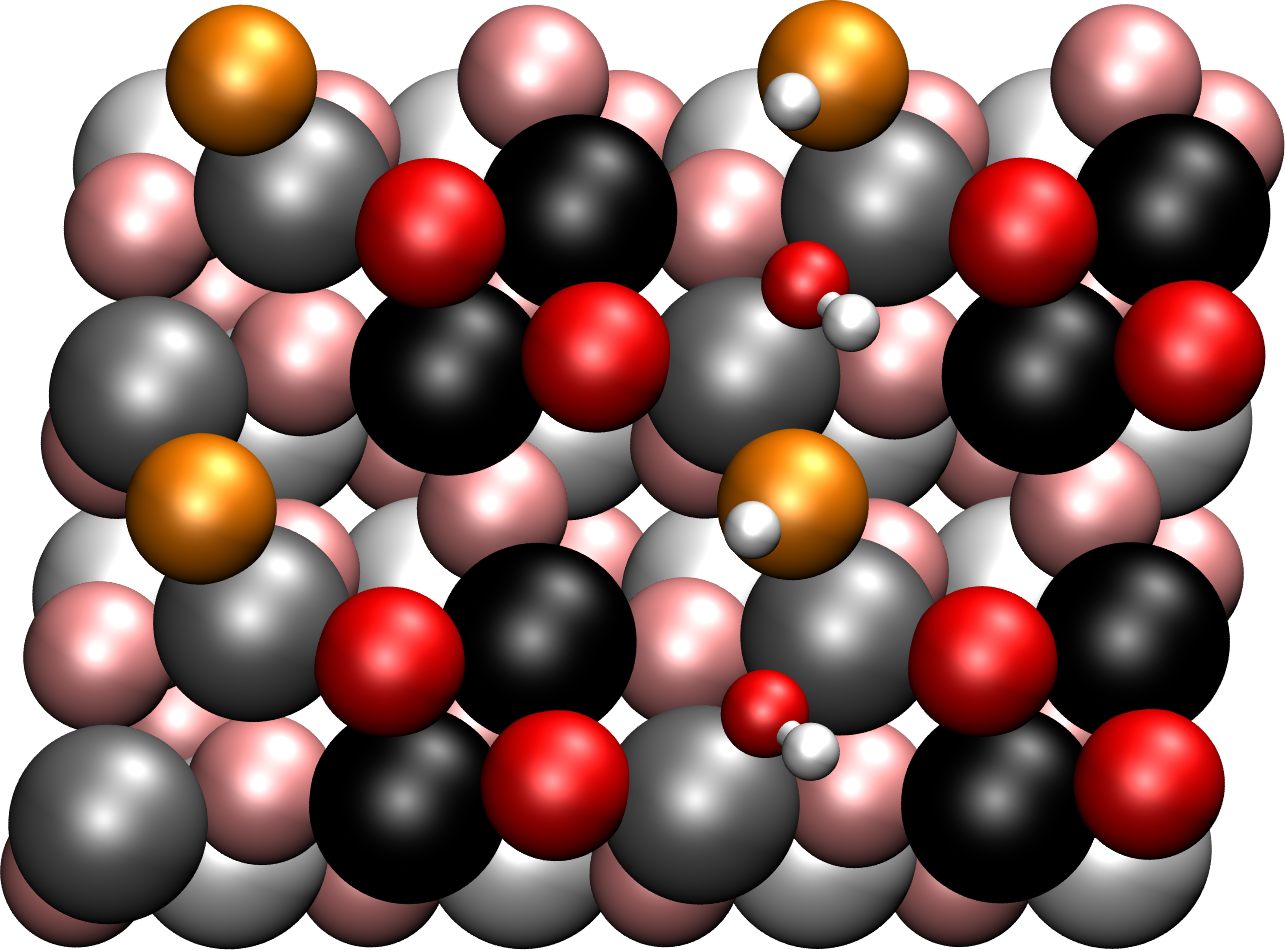
\includegraphics[width=0.302\textwidth]{figures/11-20/iCa2-iCa2.png}}
 \quad
 \caption{PBE+D2 optimized geometries of systems with two water adsorbates: (a) molecular CUSb and CUSb$\parallel$O-$\mu_2$, (b) the two most stable configurations inter-CUSa||O-$\mu_2$ and CUSb$\parallel$O-$\mu_2$ and (c) 2 inter-CUSa||O-$\mu_2$, which is the most stable adsorption pattern.}
        \label{abb:2water}
 \end{figure}
 \begin{figure}[!ht]
 \centering
\subfigure[4inter-CUSa||O-$\mu_2$]{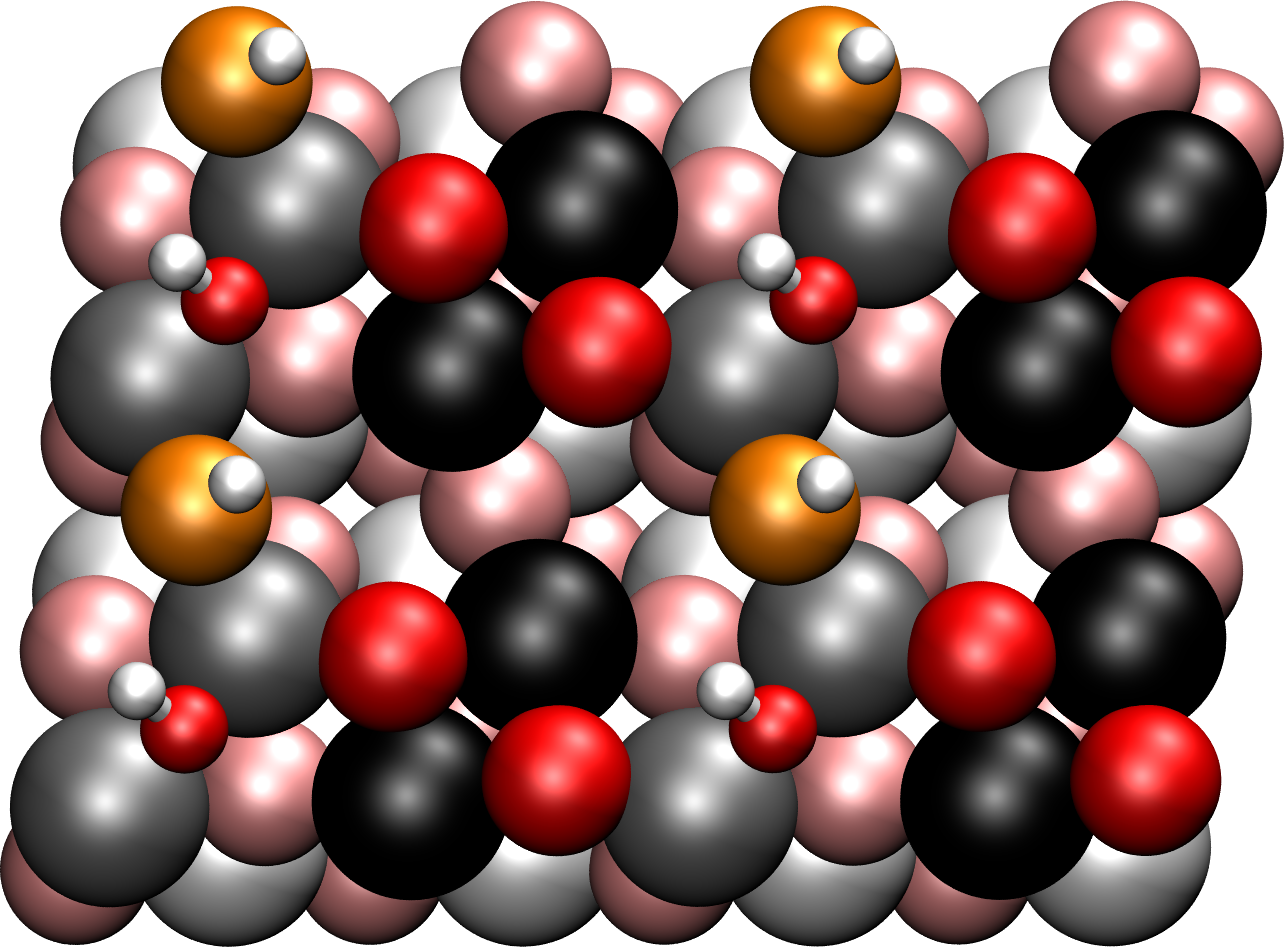
\includegraphics[width=0.4\textwidth]{figures/11-20/4iCa2.png}}
 \quad\quad
 \subfigure[1ML]{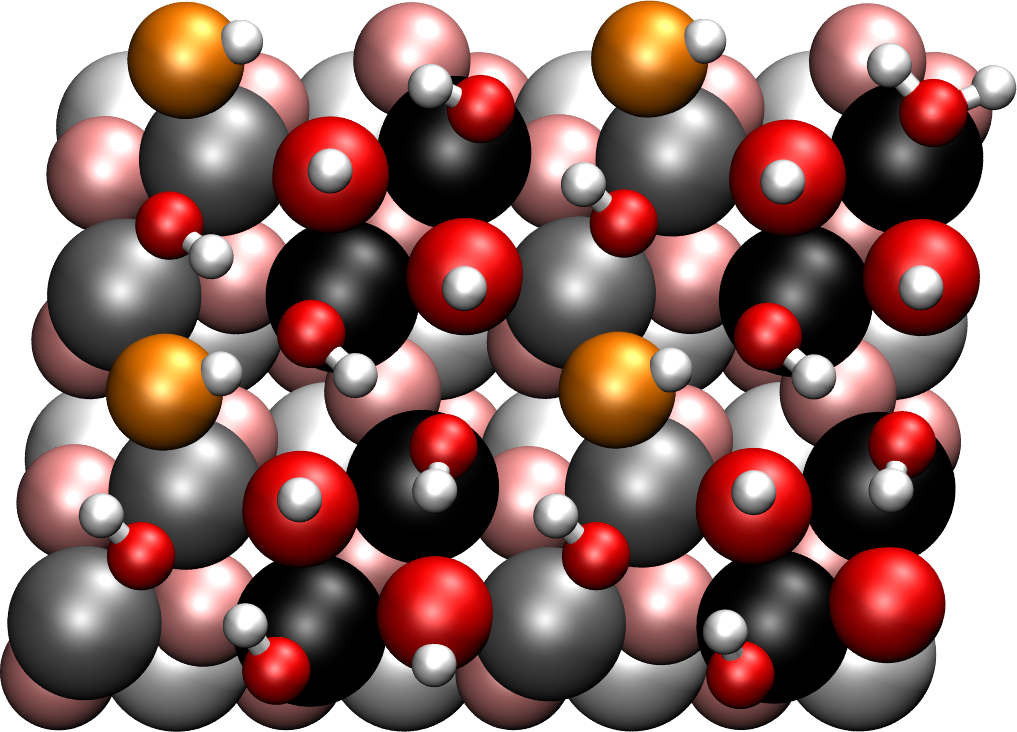
\includegraphics[width=0.4\textwidth]{figures/11-20/O-I-fully.png}}
 \caption{Optimized structures of the (a) 4 inter-CUSa$\parallel$O-$\mu_2$ and (b) fully covered (1ML) system. The latter one shows one molecular species and several hydrogen bonded OH groups.}
        \label{abb:4+fully}
 \end{figure}

The stability of those species with $n$ adsorbed water molecules is defined as
\begin{equation}
 E_\textrm{ads}=E_\text{ads. species}-(n\times E_\text{free water molecule}+E_\text{surface}).
\end{equation}
In Table \ref{tab:higher_water}, the adsorption energies for the high coverage species mentioned above are given.
\begin{table}[!ht]
  \centering
 \caption{Adsorption energies for higher water coverages in eV. For better comparison in the third column labeled ``isolated species'' the added energies for singly adsorbed water as given in Table \ref{tab:ads_1water} are presented.
\vspace*{.2cm} 
  }
  \begin{tabular}{lcc}
  Adsorbed Species  & $E_\text{ads}$ &isolated species \\
   CUSb(mol)+CUSb||O-$\mu_2$ & -4.57 & -4.06\\
   inter-CUSa||O-$\mu_2$+CUSb||O-$\mu_2$ & -4.77 & -4.78\\
   2inter-CUSa||O-$\mu_2$& -4.84 &-5.0 \\\hline
   4inter-CUSa||O-$\mu_2$ & -9.55 & -10.0\\\hline
   12H$_2$O & -23.39& $a$\tnote{a} \\
  \end{tabular}
  \label{tab:higher_water}
  \begin{tablenotes}\footnotesize 
    \item[a] $a$ One can not distinguish exactly, but there are 4 inter-CUSa-OD groups, 8 CUSb-OD groups, 8 O-$\mu_3$ and 4 O-$\mu_2$ OD groups, hence one can not calculate a sum of the isolated species.
  \end{tablenotes}

\end{table}
There are also the results for the higher coverages in comparison to results in the low overage limit by adding them up (see also column 3 in Table \ref{tab:higher_water}).
The neighborhood effect shows three different outcomes: it can have a stabilizing effect, where the dissociated water stabilizes the molecularly adsorbed water in CUSb(mol)+CUSb||O-$\mu_2$ (Figure \ref{abb:2water}(a)). It can also have the contrary effect, as can be seen in the  2inter-CUSa||O-$\mu_2$, which becomes less stable (Figure \ref{abb:2water}(c)). On the other hand, there is the inter-CUSa||O-$\mu_2$+CUSb||O-$\mu_2$ which is merely affected by the neighbor water residues (Figure \ref{abb:2water}(b)).
\\
\\
As a short excursus, also a ``defect site'', the O-II terminated surface, as it is called in the nomenclature of Kurita\cite{kuri10}, was calculated. As for the O-I termination, 10 layers were considered and from these the lowest five layers were kept fixed to bulk values. Both the clean surface and the fully covered ($1\,$ML) surface were optimized (see Figure \ref{abb:O-II-geom}) and frequency calculations were conducted, to obtain a spectrum. The structure of the clean surface, of course, differs by the ``missing'' oxygen O-$\mu_2$ atom in the topmost layer, and the fully covered system is even more different: of 12 water molecules that can adsorb, 7 adsorb molecularly and 5 dissociatively. In comparison, the fully covered system for the O-I termination only shows one molecularly adsorbed molecule.
 \begin{figure}[!ht]
 \centering
\subfigure[clean O-II surface]{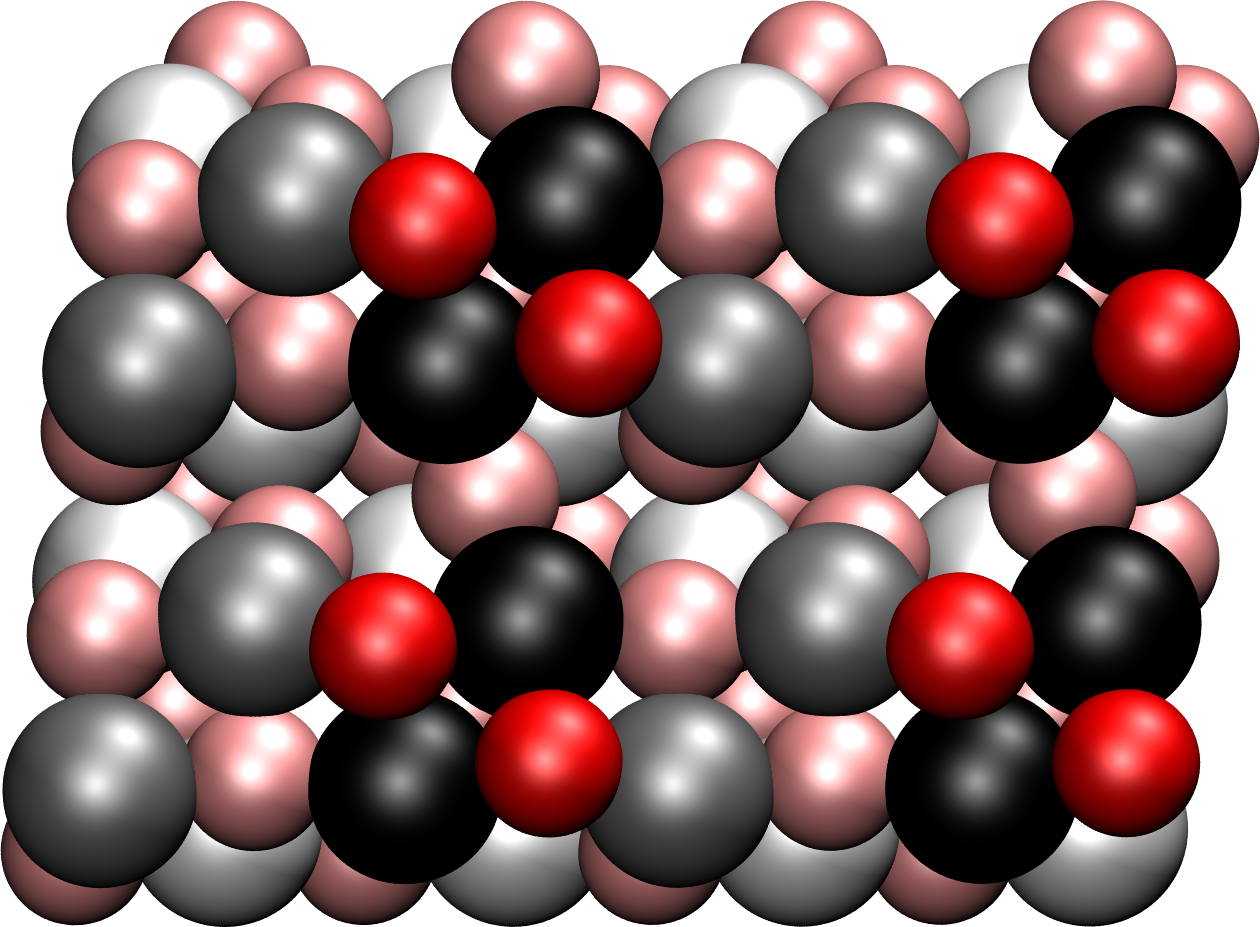
\includegraphics[width=0.4\textwidth]{figures/11-20/O-II-clean.png}}
 \quad\quad
 \subfigure[fully covered O-II surface]{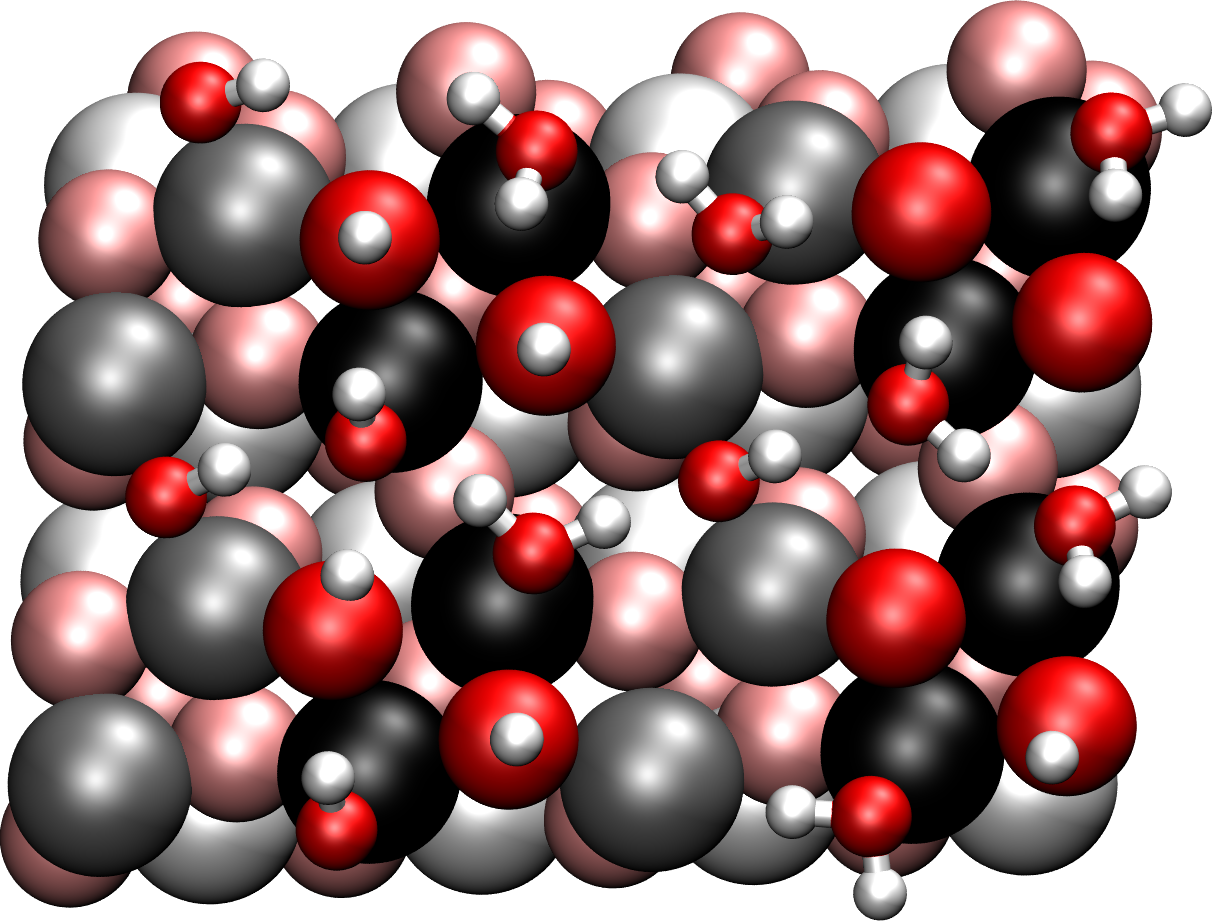
\includegraphics[width=0.4\textwidth]{figures/11-20/O-II-fully.png}}
 \caption{O-II terminated surface, as an example of a defect site optimized with PBE+D2. The top layer oxygen atom from the O-I terminated surface is missing and gives rise to a different chemical behaviour. (a) clean surface, (b) 1ML water adsorbed surface.}
        \label{abb:O-II-geom}
 \end{figure}

\section{Reactions and Microkinetic Model}\label{reactions}
\todo{discrepancy between OD and Df-OH etc. this should be consistent! In fact paths and rates were calculated for H$_2$O.}\\
Based on the minimum structures one has to identify reaction pathways to fully understand the reactivity of a system.  We utilize the NEB method including Climbing Image to search for transition states between the minima. We examined 3 different types of reactions: dissociation from the molecular minimum, as well as OH- and H-diffusion. The dissociation reactions are named D, diffusion reaction with Df-OH and Df-H, respectively, in Table \ref{tab:reaction-rates} and figures \ref{mep} and \ref{mep2}. In addition, molecular water diffusion on the surface is supposable but due to the low stability, it will dissociate before diffusion can occur. In reference \cite{Heiden11-20_2018} only some reactions were introduced, additional reactions paths are given here.
\\
We investigated 5 different dissociation reactions: the reactions from CUSb to the twofold coordinated oxygen (D-a) and one to the threefold coordinated O (D-b). One additional dissociation starts from the metastable inter-CUSa molecular structure that is, as was shown before, no minimum structure and goes to the most stable species inter-CUSa$\parallel$O-$\mu_2$ (D-c). Two further dissociation reactions were converged but showed a two step process and are therefore not interesting in the first place (these reactions are CUSb$\rightarrow$inter-CUSa$\parallel$O-$\mu_2$ and CUSb$\rightarrow$inter-CUSb$\parallel$O-$\mu_2$ and both went via the dissociated CUSb$\parallel$O-$\mu_2$ intermediate).
\\
As can be seen from section \ref{structure_search11-20} (Table \ref{tab:ads_1water}), the molecular minimum CUSb is very low in stability compared to the dissociated minima. The reaction D-a leads from the molecular minimum at CUSb to the twofold coordinated CUSb$\parallel$O-$\mu_2$:
 \begin{equation}
 \text{H$_2$O(CUSb)} \rightarrow \text{OH(CUSb)} + \text{H(O-$\mu_2$)} \tag{D-a}
      \label{dissa}
\end{equation}
The barrier is very low, about $0.002\,$eV as one can see from Table \ref{tab:reaction-rates} and Figure \ref{mep}(a), hence the reaction rate constant is very high, in the range of $k_{\text{300K}}=10^{12}\,$s$^{-1}$. This low barrier might be due to underestimation of barrier heights\cite{Zhao05} with the used functional PBE (compare section \ref{theorybeyond}).
\\ 
For the other dissociation reaction D-b from CUSb to CUSb$\parallel$O-$\mu_3$, there is no barrier found at all, the reaction pathway shows simply an upgoing path in energy without any barrier (see Figure \ref{mep}(b)), since the molecular minimum is by $0.15\,$eV more stable than the dissociated structure on CUSb$\parallel$O-$\mu_3$. Thus, no reaction rate constant can be calculated.
\begin{equation}
  \text{H$_2$O(CUSb)} \rightarrow \text{OH(CUSb)} + \text{H(O-$\mu_3$)} \tag{D-b}
      \label{dissb}
\end{equation}
A further dissociation D-c from the metastable inter-CUSa species also shows no barrier (without Figure), assumingly because the educt is no stable minimum and because the product is much more stable:
\begin{equation}
  \text{H$_2$O(inter-CUSa)} \rightarrow \text{OH(inter-CUSa)} + \text{H(O-$\mu_2$)} \tag{D-c}
      \label{dissc}
\end{equation}
On the other hand reaction D-b does also not possess a barrier, so it remains unclear whether it is due to methodology and the barrier is too low to be detected with the settings applied for the calculations or for chemical reasons.
\\
Apart from dissociation that is highly favored on this surface cut compared to more stable alumina surfaces\cite{Heiden11-20_2018}, diffusion reactions starting from the dissociated species are important for understanding for further processes.
The OD diffusion reaction Df-OH-a moves from CUSb$\parallel$O-$\mu_2$ to the inter-CUSb position, which is relatively fast for OD diffusion reactions compared to the reactions at other alumina surfaces\cite{WirthJPCC2012,Wirth2016}.
\begin{equation}
 \text{OH(CUSb)} + \text{H(O-$\mu_2$)} \rightarrow \text{OH(inter-CUSb)} + \text{H(O-$\mu_2$)} \tag{Df-OH-a}
     \label{diffOHa}
\end{equation}
In this special reaction, the OH residue diffuses from an on top CUS position into a gap between two CUSb atoms (inter-CUSb position), so that there is not much repulsion with neighboring surface oxygen atoms and other CUS atoms nearby during the diffusion, see Figure \ref{mep}(c). Also the distance that has to be overcome is very small. The barrier height equals $0.35\,$eV and the corresponding rate constant $k_{\text{300K}}=1.88\times 10^6$s$^{-1}$.
In contrast to that the real CUS-to-CUS reaction Df-OH-b that is much slower. It is a diffusion from CUSb to inter-CUSa with the hydrogen residue staying at an O-$\mu_2$ position (see Figure \ref{mep}(d)). This barrier is with $1.07\,$eV relatively high and leads to $k_{\text{300K}}=2.41\times 10^{-6}$s$^{-1}$.
\begin{equation}
 \text{OH(CUSb)} + \text{H(O-$\mu_2$)} \rightarrow \text{OH(inter-CUSa)} + \text{H(O-$\mu_2$)} \tag{Df-OH-b}
     \label{diffOHb}
\end{equation}
This is still faster than OH diffusion reaction for the (0001) alumina surface\cite{WirthJPCC2012,Wirth2014thesis}, where the rate constant $k_{\text{300K}}=4\times 10^{-45}$s$^{-1}$.
For the (1\=102) surface no OH diffusion was calculated, but the corresponding H$_2$O diffusion process is around $k_{\text{300K}}=1.4\times 10^{-3}$s$^{-1}$, whereas the H$_2$O diffusion process for the (0001) surface is in the range of $k_{\text{300K}}=8\times 10^{-3}$s$^{-1}$, too. For the (11\=20) surface no H$_2$O diffusion reactions can be observed due to the instability of the molecularly adsorbed species that would rather dissociate than diffuse.
\\
A larger variety can be achieved looking at H diffusion reactions. The different types of surface oxygen atoms and also the distances between OH and H residue make differences in the adsorption energy and also in the observed reactions.
As seen before, the hydrogen is preferably found on the twofold coordinated oxygen atom, but the reaction to a neighboring threefold coordinated oxygen is possible and opens the gate to structures with greater distance. The reaction can take place with the OH residue being on a CUSb site:
\begin{equation}
 \text{OH(CUSb)} + \text{H(O-$\mu_2$)} \rightarrow \text{OH(CUSb)} + \text{H(O-$\mu_3$)} \tag{Df-H-a}
     \label{diffHa}
\end{equation}
The reaction shows a proton transfer reaction with a barrier height of $0.95\,$eV, but the NEB transition state has no imaginary frequency so that no rate can be derived, although the NEB path clearly shows a smooth barrier profile, compare Figure \ref{mep2}(a).
\\
A further reaction starting from the most stable inter-CUSa$\parallel$O-$\mu_2$ to the threefold coordinated oxygen can be seen in Figure \ref{mep2}(b) and is called reaction Df-H-b:
\begin{equation}
 \text{OH(inter-CUSa)} + \text{H(O-$\mu_2$)} \rightarrow \text{OH(inter-CUSa)} + \text{H(O-$\mu_3^\prime$)} \tag{Df-H-b}
     \label{diffHb}
\end{equation}
The barrier of the free energy is $1.50\,$eV, with a rate constant at $300\,$K of $4.90\times 10^{-13}$s$^{-1}$. This process is so unlikely because a less favored O-$\mu_3$ position is occcupied and this position is also less stabilized by reason of the greater distance of OH$_{\text{surf}}$ and OH$_{\text{ads}}$ groups. This reaction increases the distance to a position further away than next neighbor.
As mentioned before, the nomenclature for these structures uses primes ($\prime$) to display the distance.
\\
A similar reaction can be seen in Figure \ref{mep2}(c) for the OH being situated on inter-CUSb and the hydrogen being adsorbed on an O-$\mu_2^{(\prime)}$ position, diffusing further away to O-$\mu_3^{\prime\prime}$, which is less in stability:
\begin{equation}
 \text{OH(inter-CUSb)} + \text{H(O-$\mu_2^{(\prime)}$)} \rightarrow \text{OH(inter-CUSb)} + \text{H(O-$\mu_3^{\prime\prime}$)} \tag{Df-H-c}
     \label{diffHc}
\end{equation}
The free energy barrier is relatively high with $1.30\,$eV giving a rate constant $k_\textrm{300K}=9.96\times 10^{-1}$s$^{-1}$. The $^\prime$ in the equation above is set in parantheses because it is the nearest possible O-$\mu_2$ position, but not the nearest possible distance from the OH$_\textrm{ads}$.

Going one step further from reaction Df-H-c, the following reaction leads to the position where OH and H have the greatest possible distance with the applied periodic bounding conditions:
\begin{equation}
 \text{OH(inter-CUSb)} + \text{H(O-$\mu_3^{\prime\prime}$)} \rightarrow \text{OH(inter-CUSb)} + \text{H(O-$\mu_3^{\prime\prime\prime}$)} \tag{Df-H-d}
     \label{diffHd}
\end{equation}
With an energy barrier of $0.94\,$eV the rate at $300\,$K is $1.1\times 10^{-3}$s$^{-1}$, see also Figure \ref{mep}(d).
\\
These H diffusion paths can be assembled to a longer diffusion path leading from inter-CUSb$\parallel$O-$\mu_3$ to O-$\mu_2^\prime$ to O-$\mu_3^{\prime\prime}$ and to the furthest possible O-$\mu_3^{\prime\prime\prime}$. The first reaction was calculated but did not converge for unknown reasons. The two next steps of this hydrogen migration path were studied (Df-H-c and Df-H-d). The rate of the first step is unknown but it is assumed to be fast, because as the product a very stable O-$\mu_2$ configuration is involved. The second reaction (Df-H-c) has a medium rate with $10^{-1}$s$^{-1}$. The last step of this path is the slowest with $10^{-3}$s$^{-1}$. The corresponding adsorption energy profile is different from that: $-1.89$, $-2.09$, $-1.16$ and $-1.22$eV. One can conclude that hydrogen migration but not likely because the O-$\mu_2$ acts as a trap for H that hinders further reactions.
\\
\begin{table*}[ht]
  \centering
  \caption{Energy and free energy differences are given:  $\Delta E=E(\textrm{product}) - E(\textrm{educt})$, $\Delta E^{\ddagger}=E^\ddagger - E(\textrm{educt})$, respective for $G$. The same is given for the transition state - educt. Thermodynamic properties are given at $T=300\,$K. $k$ is the rate constant from eq.~(\ref{eq:eyring}). The three types of reactions are dissociation (D), OH diffusion (Df-OH) and H diffusion (Df-H). ``n.f.'' indicates ``not found''}
  \begin{tabular}{cl|cc|cc|c}
  \multicolumn{2}{c|}{\small{Reaction Type}}             & \small{$\Delta E$(eV)}& \small{$\Delta G_\text{300 K}$(eV)} & \small{$\Delta E^{\ddagger}$(eV)} & \small{$\Delta G_\text{300 K}^{\ddagger}$(eV)} & \small{$k_\text{300 K}$(s$^{-1}$)}  \\
    \hline
\multirow{3}{*}{\small{\ce{H2O} dissociation}} &
   \small{D-a}  & \small{-0.50} & \small{-0.52} & \small{0.01} & \small{0.002} & \small{5.76$\times 10^{12}$} \\
 & \small{D-b} & \small{0.59} & \small{0.53} & \small{n.f.} & \small{n.f.} & \small{n.f.} \\
 & \small{D-c} &\textit{\small{-1.15}} &\textit{\small{-1.27}} & \small{n.f.} & \small{n.f.} & \small{n.f.}  \\
    \hline
 \multirow{2}{*}{\small{OH diffusion}} &
   \small{Df-OH-a} & \small{0.19} & \small{0.22} & \small{0.35} & \small{0.39} & \small{1.88 $\times  10^6$}\\
 & \small{Df-OH-b}  & \small{-0.21} & \small{-0.13} & \small{1.07} & \small{1.10} & \small{2.41$\times 10^{-6}$} \\
    \hline
\multirow{4}{*}{\small{H diffusion}} &
  \small{Df-H-a} &\textit{\small{0.76}} &\textit{\small{0.58}} & \small{n.f.}&\small{n.f.} & \small{n.f.}\\
& \small{Df-H-b}  & \small{1.08} & \small{1.04} & \small{1.65} & \small{1.49} & \small{4.90$\times 10^{-13}$} \\
& \small{Df-H-c} & \small{0.93} & \small{0.89} & \small{1.36} & \small{1.30} & \small{9.96$\times 10^{-10}$}\\
& \small{Df-H-d} & \small{-0.06} & \small{-0.07} & \small{1.05} & \small{0.94} & \small{1.05$\times 10^{-3}$} \\
  \end{tabular}
  \label{tab:reaction-rates}
\end{table*}
\\
Proton diffusion reactions are way more variable than OH diffusions or dissociation reactions, providing reaction rates at $300\,$K ranging from $10^{-13}$ to $10^{-3}$s$^{-1}$. The barriers and therefore also rate constants for H-diffusion cover a wider range depending on the distance between OH and H and of course more importantly on the fact between which types of O-$\mu_{2/3}$ the proton is diffusing.
\\
Also reactions leading to another situation than next neighbored, increasing the distance between OH and H are less favorable since geometries with the residues further apart are energetically less stable (compare Table \ref{tab:ads_1waterfurther}).
\begin{figure*} [!ht]
\centering
\subfigure[D-a: CUSb $\rightarrow$CUSb||O-$\mu_2$]{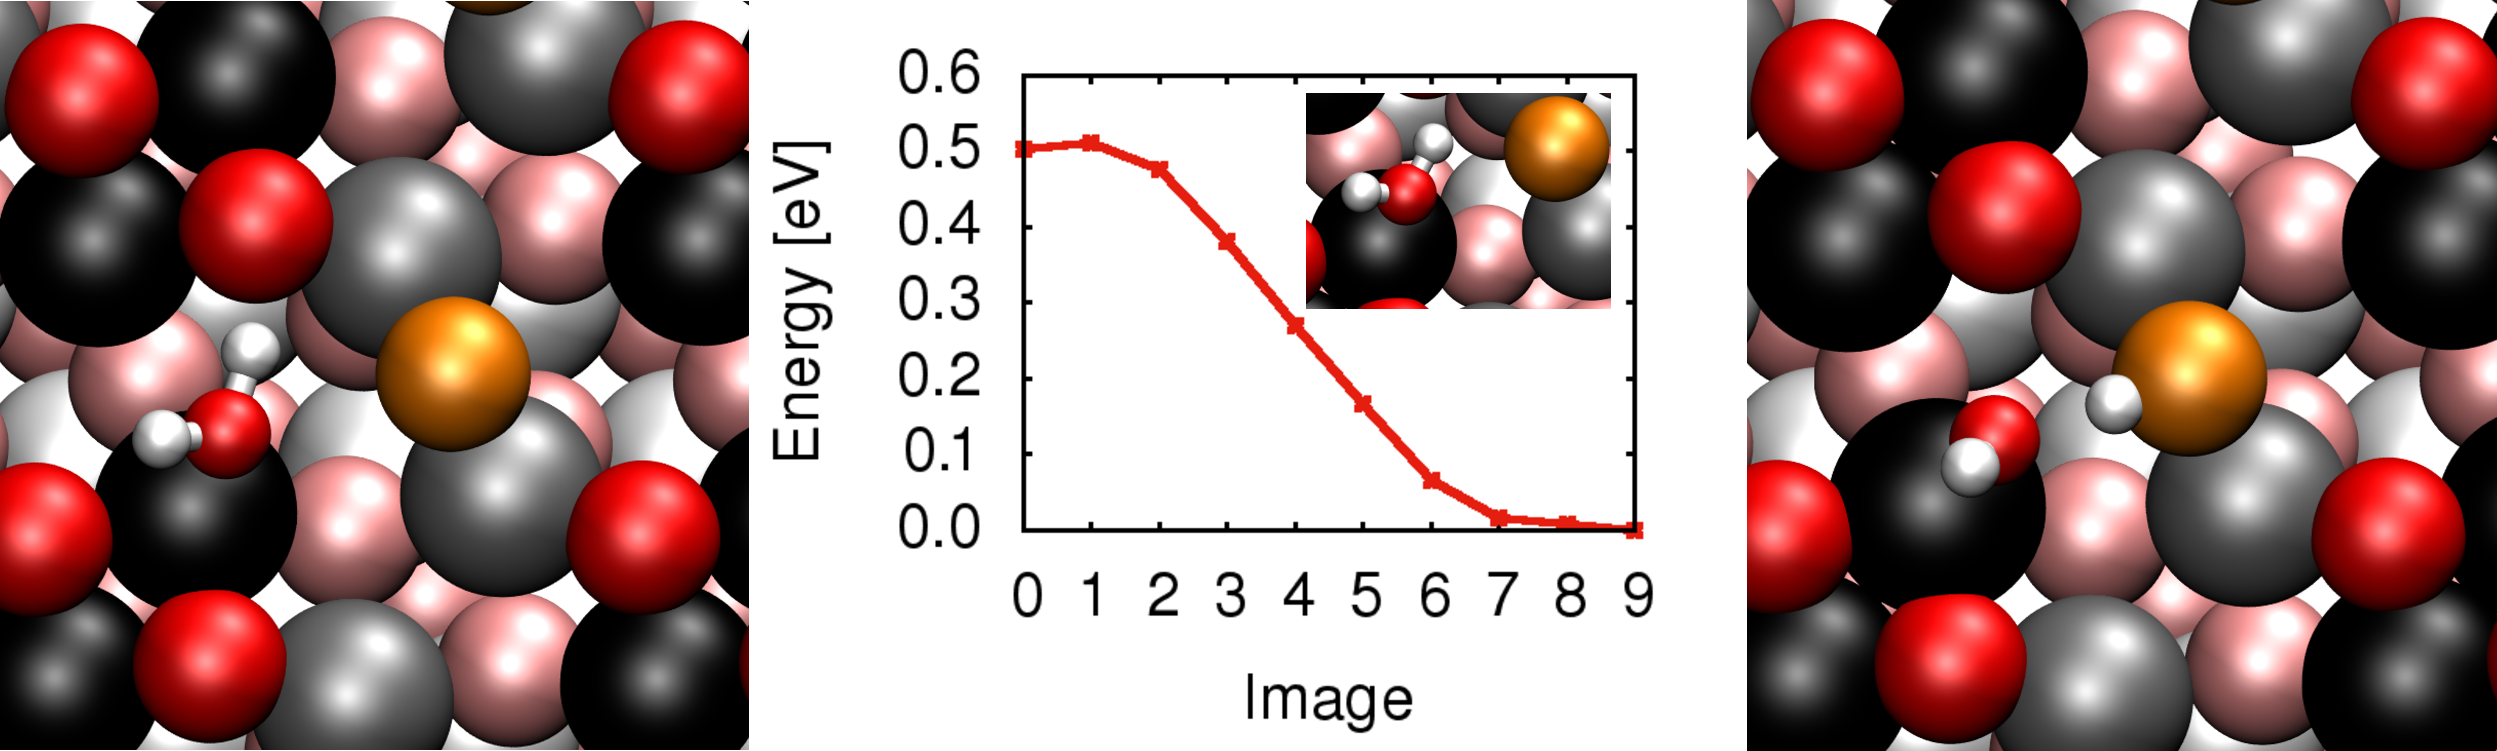
\includegraphics[width=0.7\textwidth]{figures/11-20/Diss_Cb-Cb2.pdf}}
         \quad
\subfigure[D-b: CUSb $\rightarrow$CUSb||O-$\mu_3$]{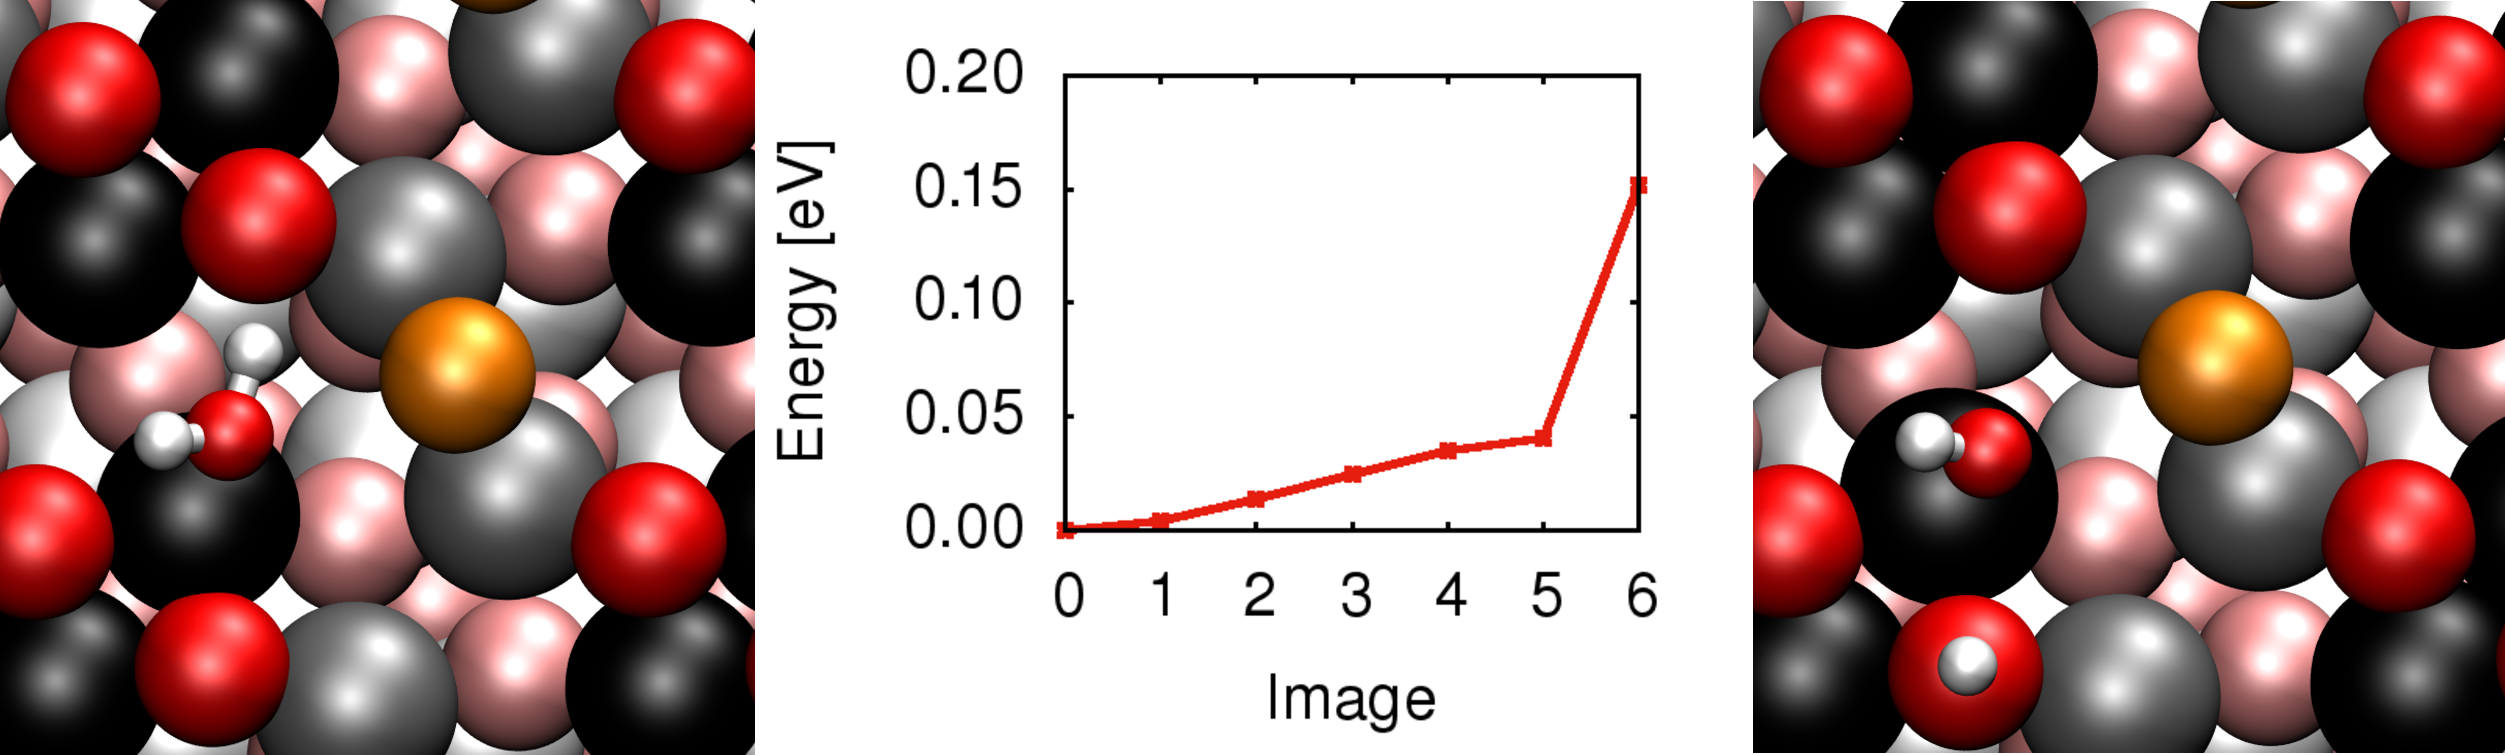
\includegraphics[width=.7\textwidth]{figures/11-20/Diss_Cb-Cb3.pdf}}
 \quad
\subfigure[Df-OH-a: CUSb||O-$\mu_2$ $\rightarrow$inter-CUSb||O-$\mu_2$]{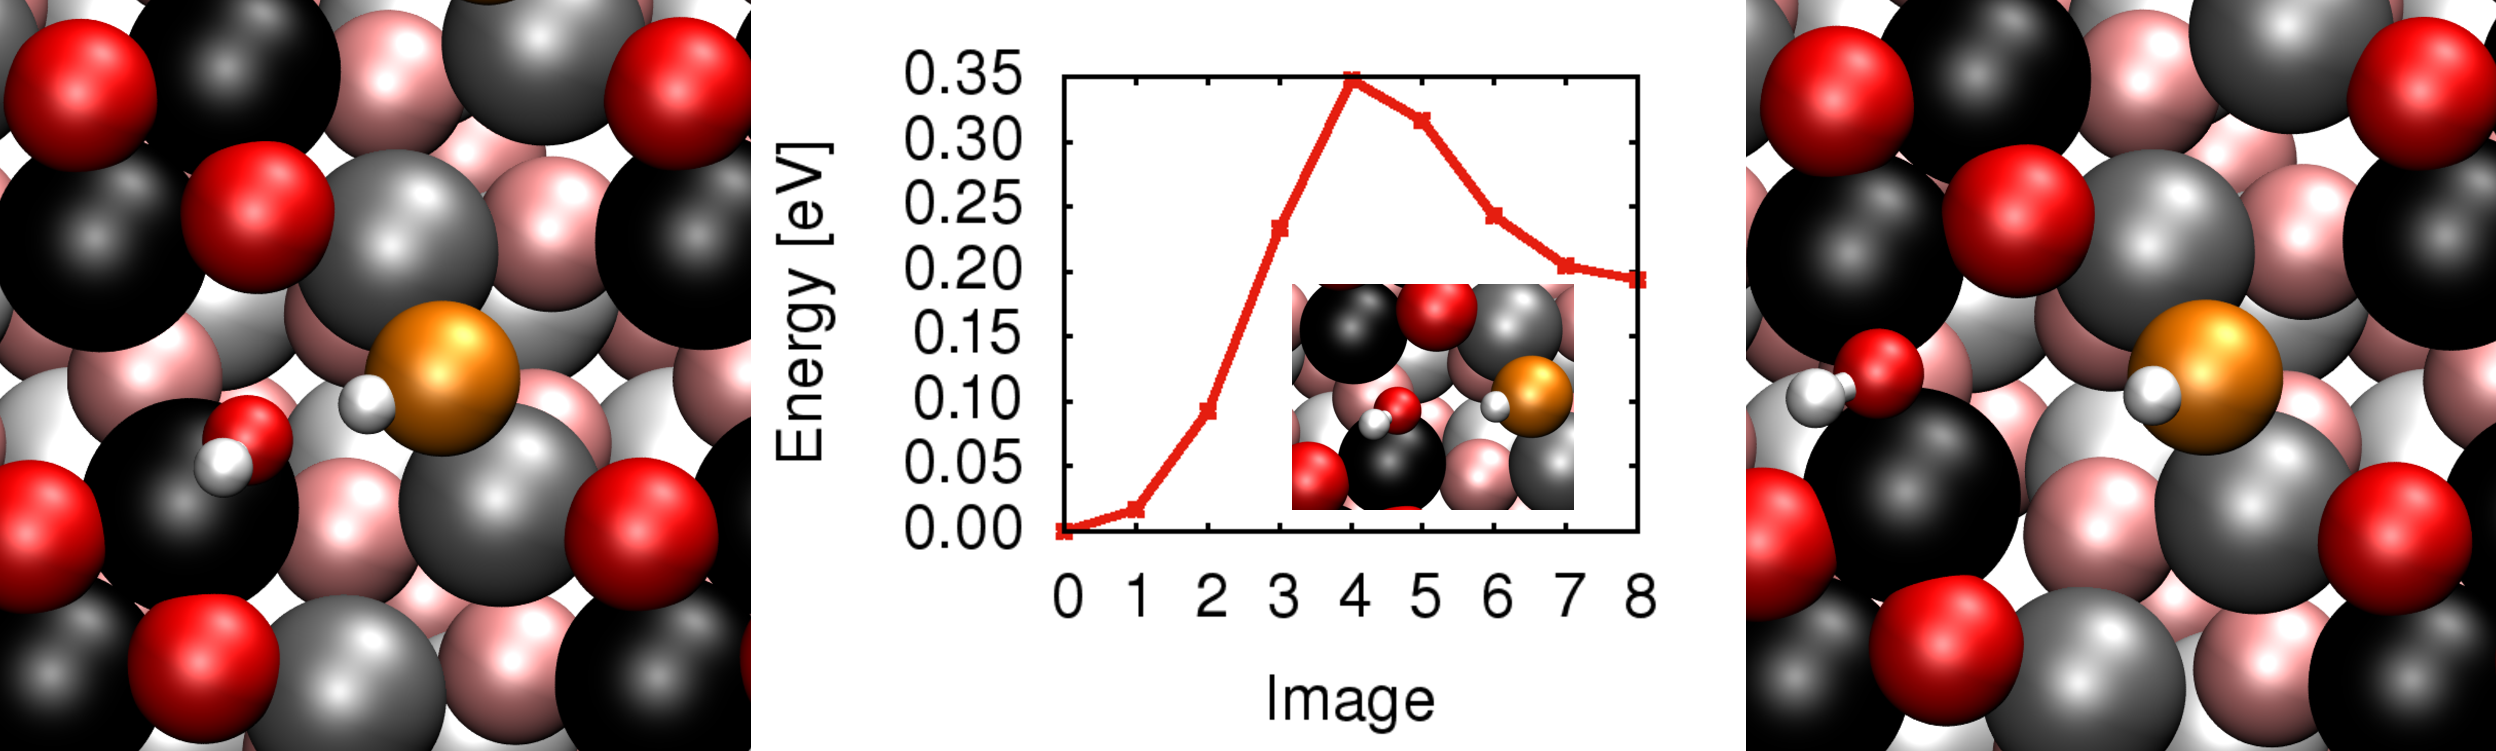
\includegraphics[width=.7\textwidth]{figures/11-20/Diff-OH_Cb2-iCb2.pdf}}
 \quad
\subfigure[Df-OH-b: CUSb||O-$\mu_2$ $\rightarrow$inter-CUSa||O-$\mu_2$]{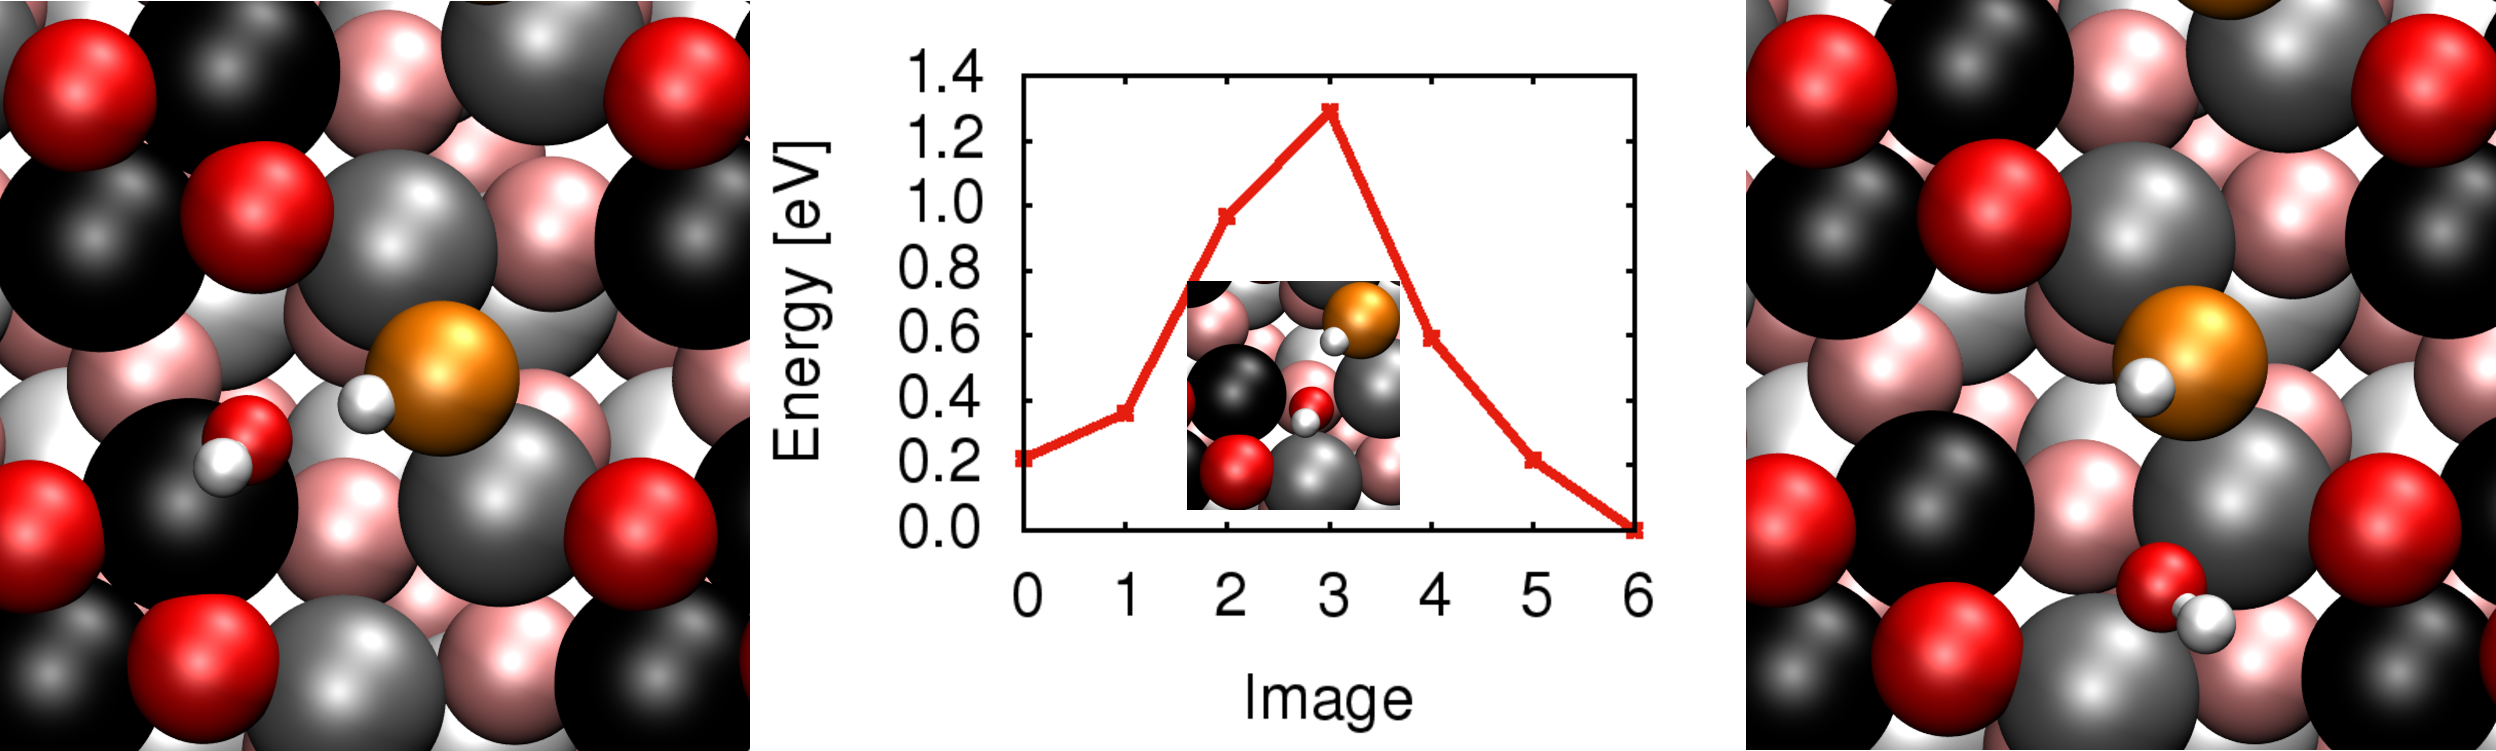
\includegraphics[width=.7\textwidth]{figures/11-20/Diff-OH_Cb2-iCa2.pdf}}
\caption{Minimum energy paths with transition states (inlay; if available), and both educt (left) and product (right) states for D-a, D-b, D-c, Df-OH-a and Df-OH-b reactions, respectively. The color code is as explained above.}
       \label{mep}
\end{figure*}
\begin{figure*} [!ht]
\centering
\subfigure[Df-H-a: CUSb||O-$\mu_2\rightarrow$CUSb||O-$\mu_3$]{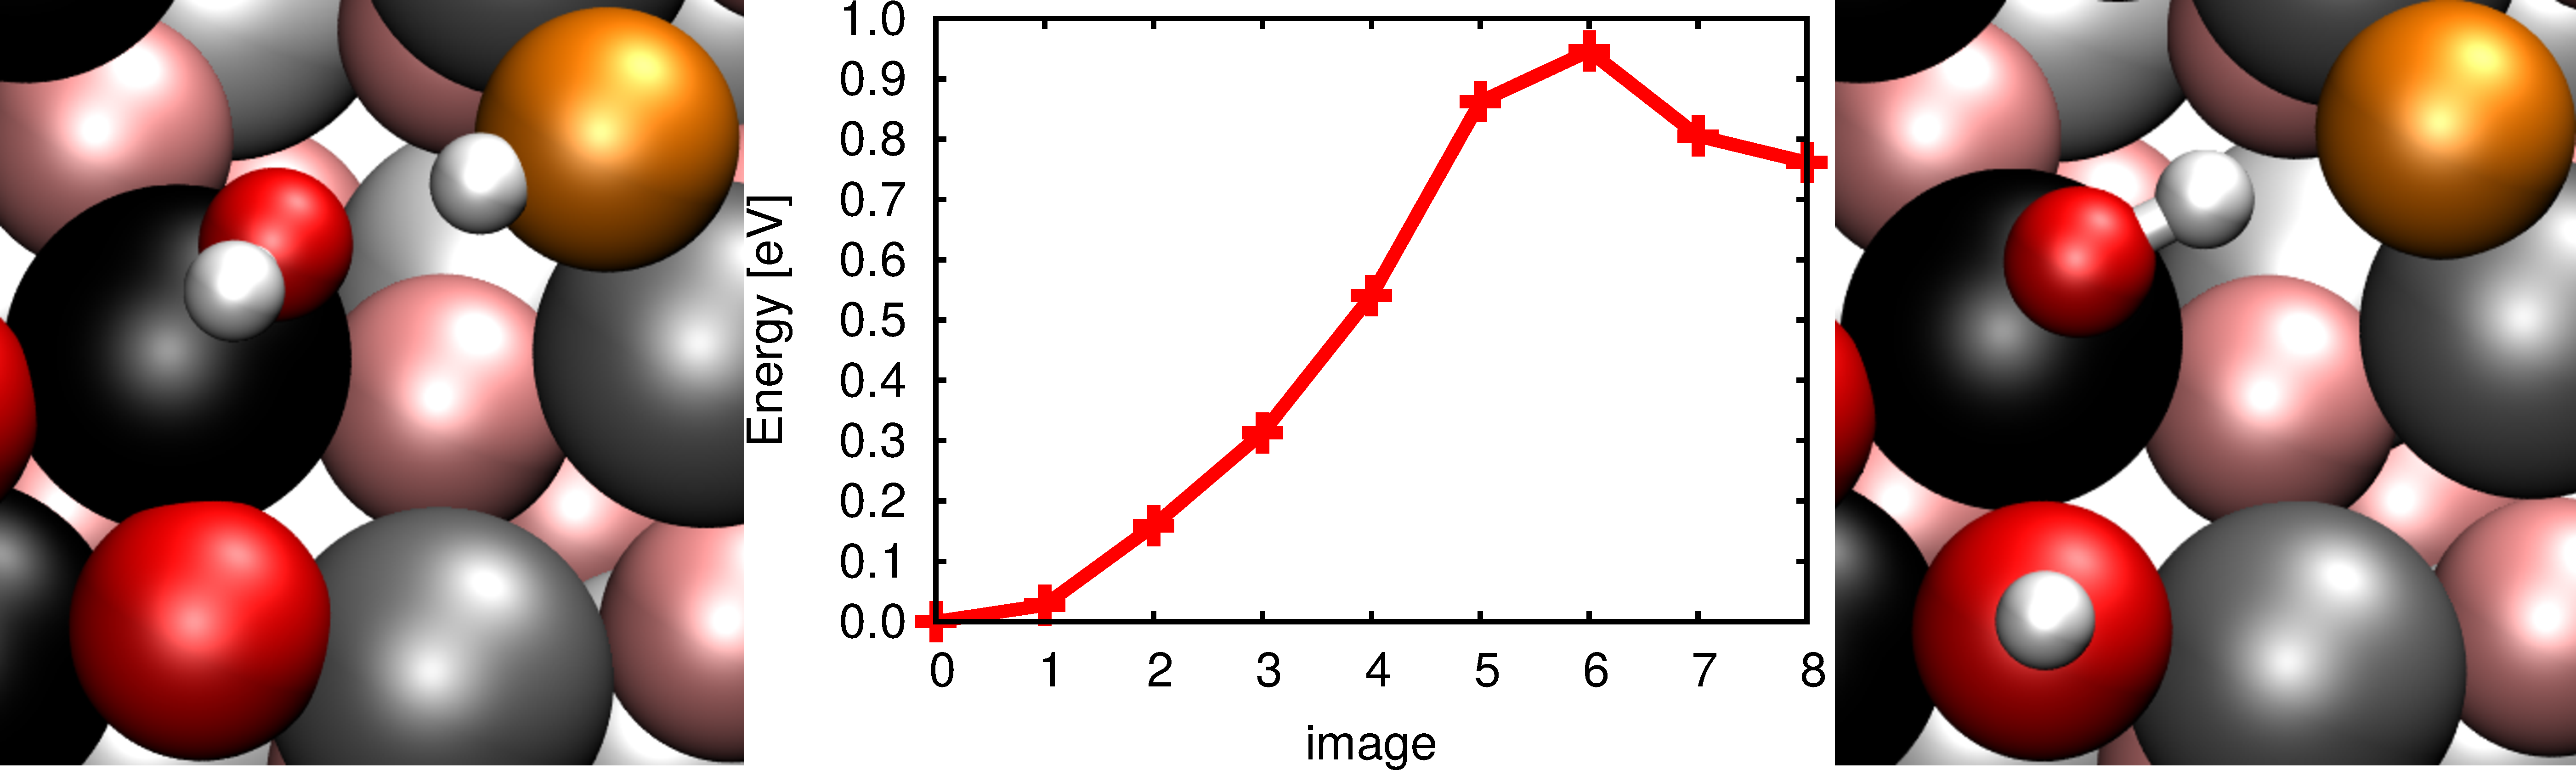
\includegraphics[width=.7\textwidth]{figures/11-20/Diff-H_Cb2-Cb3.pdf}}
\quad
\subfigure[Df-H-b: inter-CUSa||O-$\mu_2\rightarrow$inter-CUSa||O-$\mu_3^\prime$]{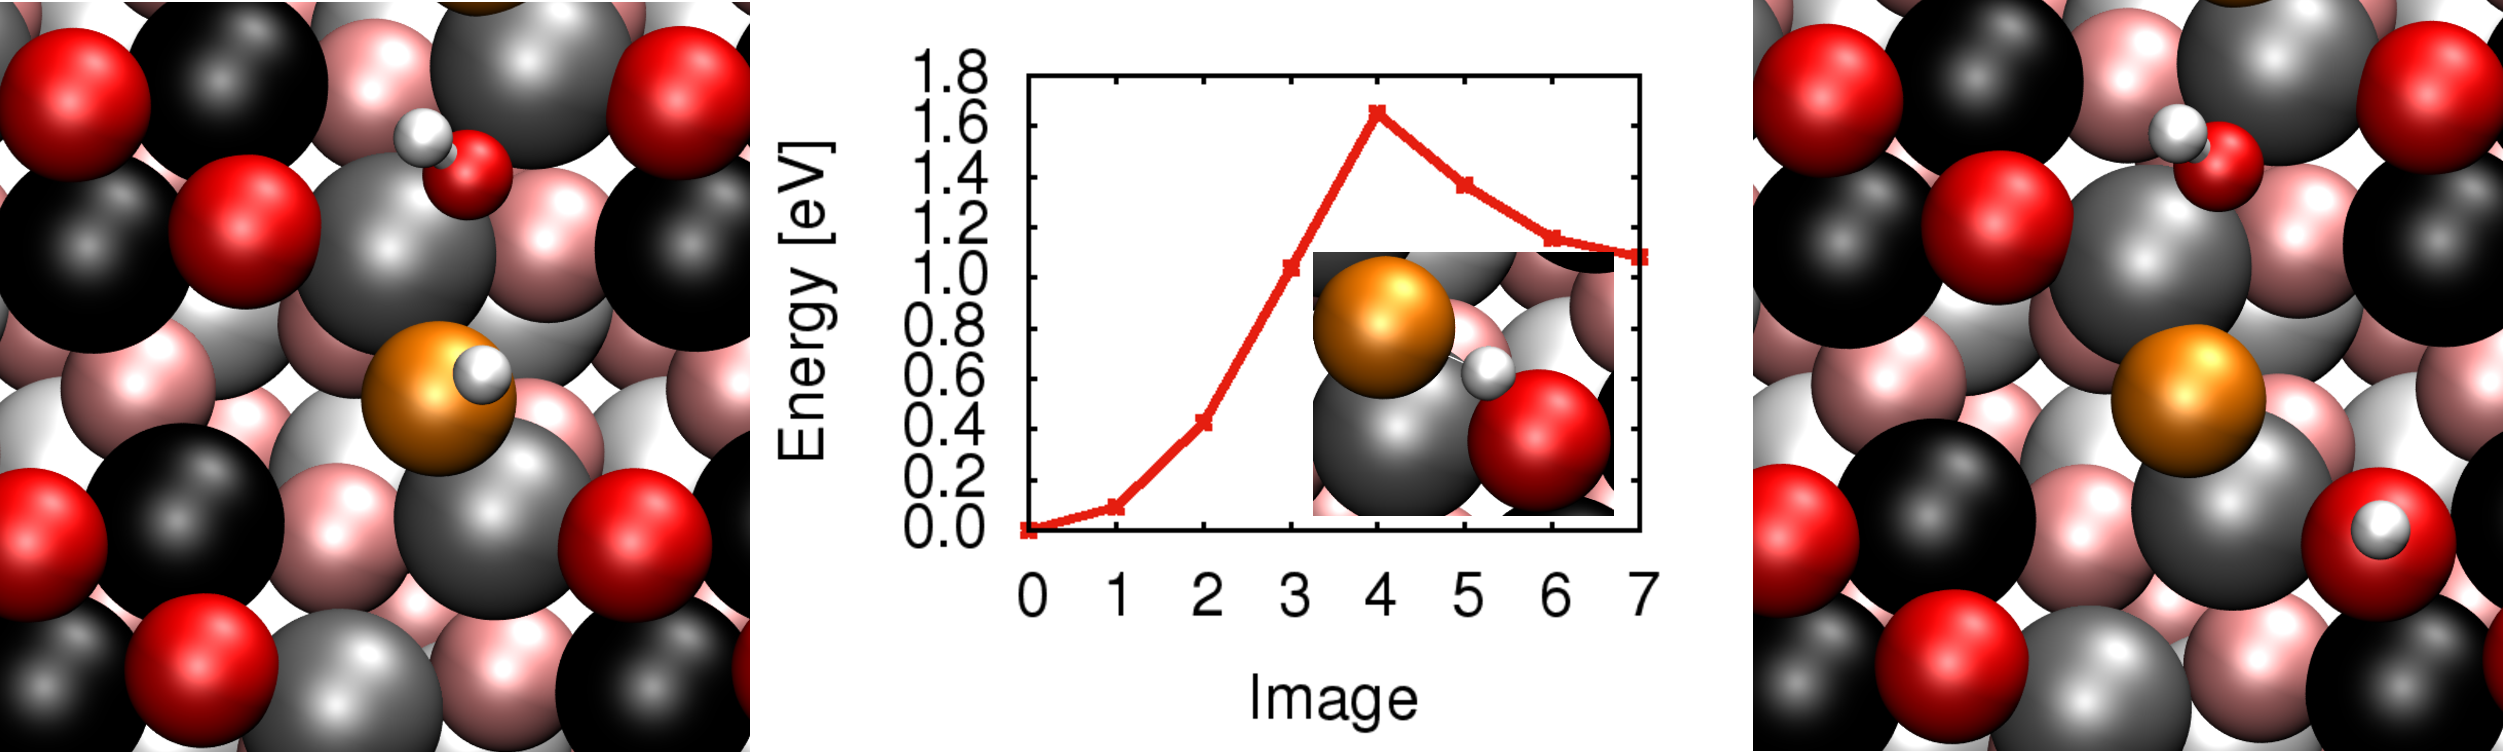
\includegraphics[width=.7\textwidth]{figures/11-20/Diff-H_iCa2-iCa3p.pdf}}
 \quad
 \subfigure[Df-H-c: inter-CUSb||O-$\mu_2^\prime\rightarrow$inter-CUSb||O-$\mu_3^{\prime\prime}$]{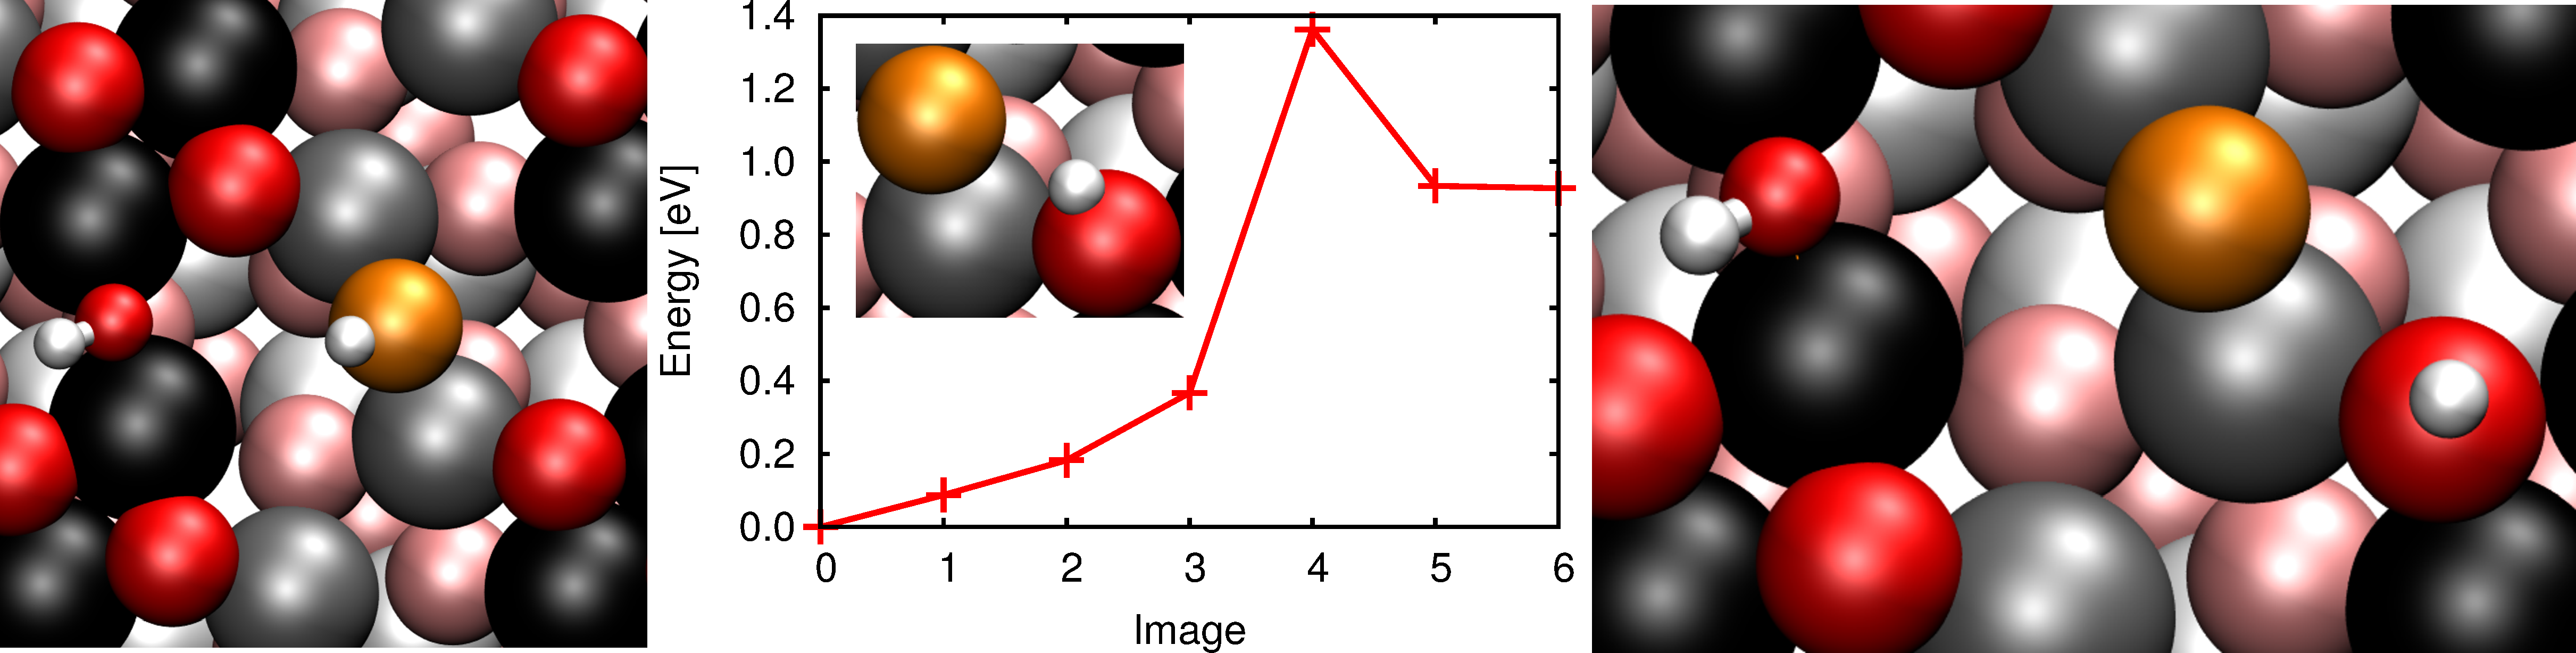
\includegraphics[width=.7\textwidth]{figures/11-20/Diff-H_iCb2p-iCb3pp.pdf}}
 \quad
\subfigure[Df-H-d: inter-CUSb||O-$\mu_3^{\prime\prime}$ $\rightarrow$inter-CUSb||O-$\mu_3^{\prime\prime\prime}$]{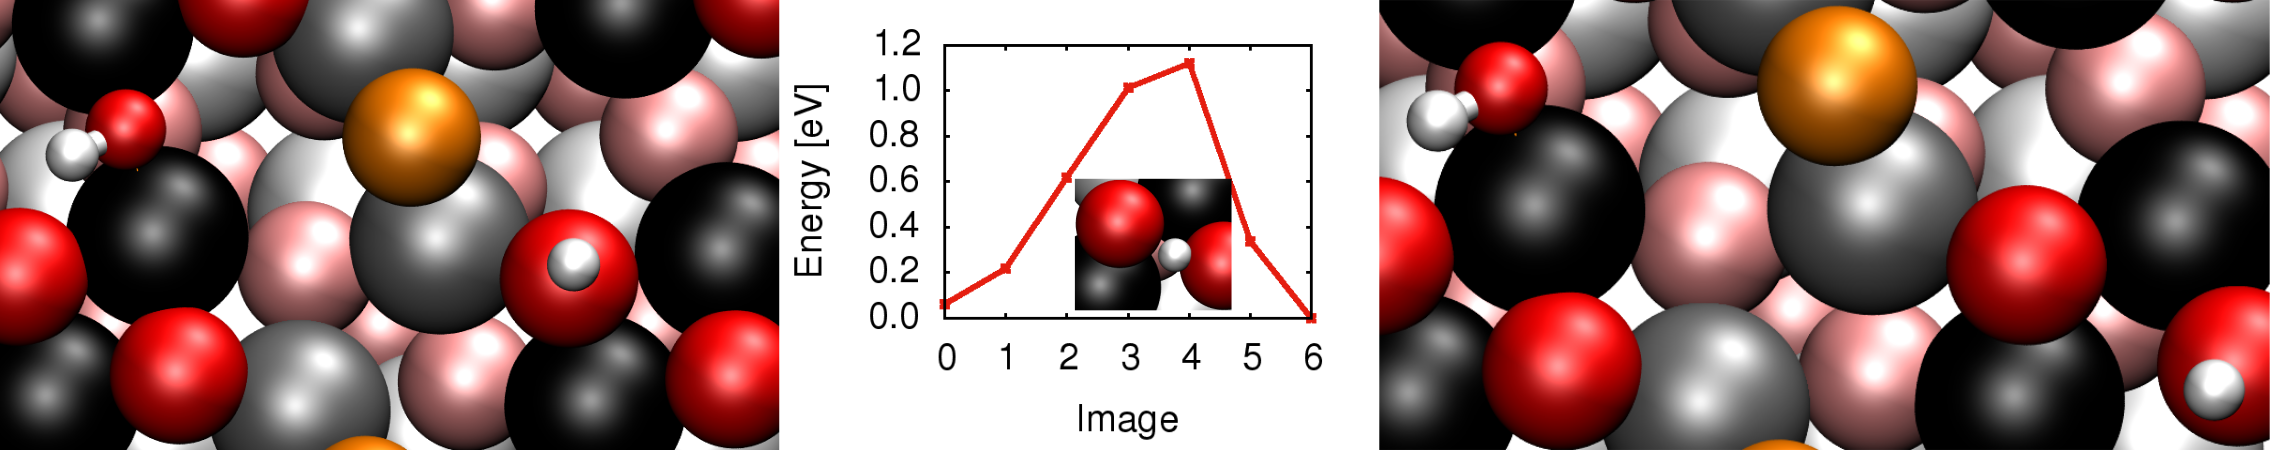
\includegraphics[width=.7\textwidth]{figures/11-20/Diff-H_iCb3pp-iCb3ppp.png}}
\caption{Minimum energy paths with transition states, and both educt and product states for Df-H-a - Df-H-d reactions. The color code is as explained above.}
       \label{mep2}
\end{figure*}

Rates for backreactions can also be calculated and the results are shown in Table \ref{tab:backreactions}.
\begin{table*}[ht]
  \centering
  \caption{Reaction rate constants for the backreactions (right) in comparison with forward reactions (left). These rates can be calculated via detailed balance $\stackrel{\leftarrow}{k}  = \stackrel{\rightarrow}{k} \ e^{-\Delta G/k_B T}$. All values are given in s$^{-1}$ at a temperature of $300\,$K.}
  \begin{tabular}{cl|cc|cc|c}
\small{Reaction Type} & \small{$k_\text{300 K}$(s$^{-1}$)} &  \small{$k_\text{300 K}$(s$^{-1}$)} \\
 &forward reaction &back reaction \\\hline
 \small{D-a}   & \small{5.76$\times 10^{12}$} &\small{1.17$\times 10^4$}\\
 \small{D-b}   & \small{n.f.} & \small{n.f.} \\
 \small{D-c}   & \small{n.f.} & \small{n.f.}  \\\hline
 \small{Df-OH-a} & \small{1.88 $\times  10^6$}&\small{9.86$\times 10^9$} \\
 \small{Df-OH-b}  & \small{2.41$\times 10^{-6}$}& \small{1.69$\times 10^{-8}$}\\\hline
 \small{Df-H-a} & \small{n.f.} &\small{n.f.} \\
 \small{Df-H-b}  & \small{4.90$\times 10^{-13}$} &\small{1.49$\times 10^5$} \\
 \small{Df-H-c} & \small{9.96$\times 10^{-10}$}& \small{9.95$\times 10^5$}\\
 \small{Df-H-d} & \small{1.05$\times 10^{-3}$} &\small{7.12$\times 10^{-5}$} \\
  \end{tabular}
  \label{tab:backreactions}
\end{table*}
\\
As mentioned before an immense well known problem of GGA is that barriers are underestimated\cite{Zhao05}. Optimizing structures with HSE06 is nearly impossible due to high cost and doing single point calculations on PBE optimized transition state is not very accurate and doesn't deliver better results (unpublished work by Dr. J. Wirth, U Potsdam). %\todo{at least for crystal calculations... so don't bring it here?}
\clearpage
\section{Vibrational Frequencies / Spectroscopic Properties}
A great source of knowledge about chemical systems is vibrational spectroscopy, so we were interested in vibrational frequencies of the systems, since the frequencies of vibrations give us hints about the chemical environment as hydrogen bonds and other atoms nearby that bond to each other. These vibrational frequencies were calculated for the surface system adsorbed with OH and also with OD. Our experimental partners from FHI use deuterated water (D$_2$O) instead of H$_2$O because the chemical reactivity is the same but the spectroscopic properties are clearer with their applied Laser system. The experimental SFG spectra (Sum Frequency Generation) for the OD range of the low coverage regime for two different coverages are shown in Figure \ref{abb:exp-sfg} as they were published in \cite{Heiden11-20_2018}.
\begin{figure}[!ht]
 \centering
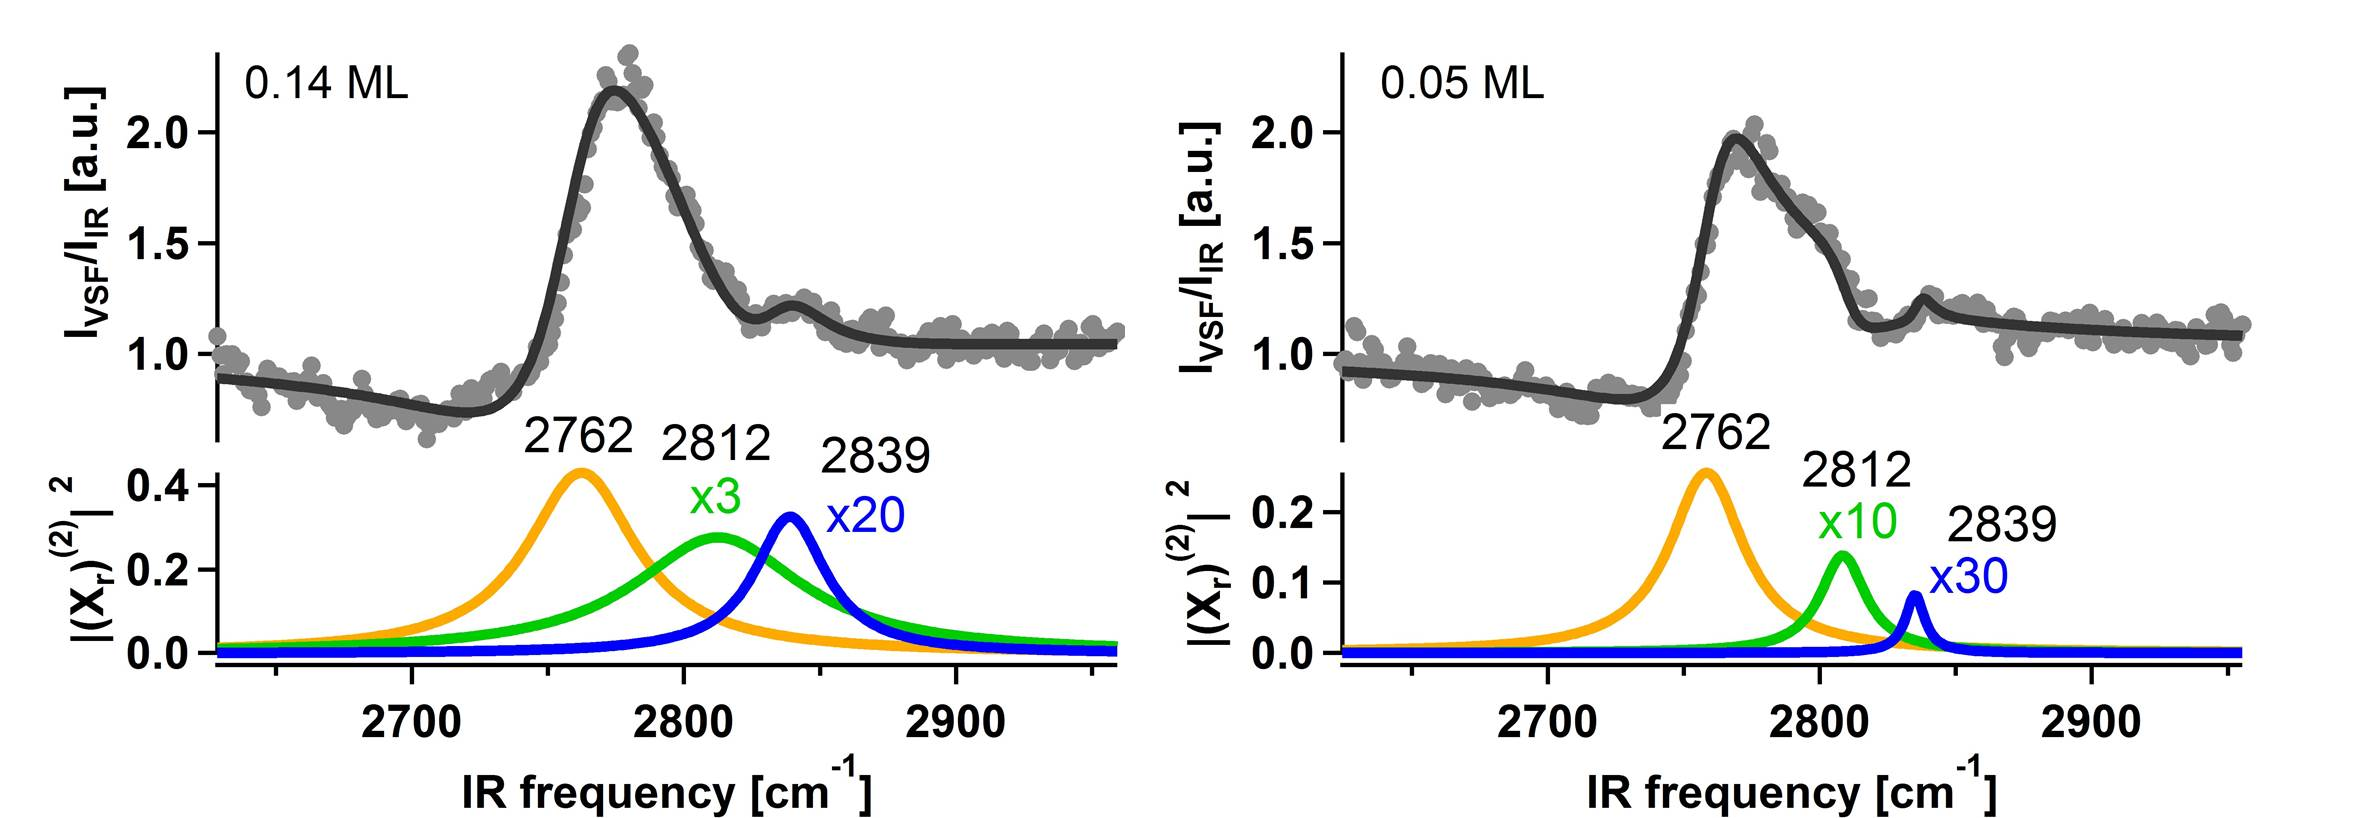
\includegraphics[width=0.9\textwidth]{figures/11-20/SFG_fit.jpg}
 \caption{Experimental SFG results for (11\=20) surface with 0.14ML (mono layer, left spectrum) and 0.05ML water coverage (right) including fit. The experiment was conducted by Yanhua Yue, FHI Berlin. Coverage only influences intensity of the peaks but not the peak position itself. The different coverages are achieved via different preparing temperatures of the sample.}
        \label{abb:exp-sfg}
 \end{figure}
Of course, the frequencies for a deuterated system are different from OH, but the different isotopes can be calculated easily within vasp, just by changing the mass.
\\
In experiment the alumina single crystal was cleaned in ethanol and Milli-Q water and dried with N$_2$ before being installed in the ultra high vacuum chamber. It was then sputtered in Ar, and annealed to high temperatures in UHV and afterwards three times in oxygen at different temperatures. After this treatment, D$_2$O was brought onto the surface with a molecular beam source. For further details see \cite{Heiden11-20_2018} and the supporting information therein.
\\
\\
To calculate the modes in this work mainly two methods were applied: Normal mode analyses (see section \ref{nma}) and power spectra from \textit{ab initio} MD via velocity-velocity autocorrelation function (section \ref{vvacf}).
\\
The focus lies mainly on the position of the peaks rather than the intensities, because in the first place it is of greater importance what kind of vibrations gives which peak than the intensity of the peak itself. Also, it is still challenging to determine the frequencies before heading to intensities.
In the power spectra from MD calculations the intensities are implicitly received and for the normal mode analyses this work follows 2 different approaches: dipole corrections and Born effective charges.
\\
In subsection \ref{nma}, also modes for higher coverage systems are also examined.
\\
But not only the OD frequencies are of interest, but also the lattice vibrations, and are covered in both subsections.

\subsection{Normal Mode Analysis}\label{nma}
\subsubsection{OD Vibrations}
The normal modes are calculated within the harmonic approximation and depend on the mass and the spring constant of the bond. This ansatz is quite good for high frequency modes like OD stretch vibrations. We assumed that the OD stretching modes for the three most stable structures would contribute to the spectrum the most. These results are presented in Table \ref{tab:freq_layers}.
\begin{table*}[th]
  \centering
 \caption{Wavenumbers of normal modes for the different slab sizes: OD stretching modes for each of the most stable minima. All values are given in cm$^{-1}$; in parantheses, the angle of the OD bonding vector to the surface normal ($\theta$ in \textdegree) is provided. In each column, the left value reflects the adsorbed OD group and the right wavenumber the surface OD group, respectively.  In the right half a sketch of the angle $\theta$ between the OD bond and the surface normal is shown.}
\vspace*{.2cm} 
 \begin{tabular}{l|ccccc}
  Layers&inter-CUSa$\parallel$O-$\mu_2$ &CUSb$\parallel$O-$\mu_2$  &inter-CUSb$\parallel$O-$\mu_2$&\multirow{6}{1pt}{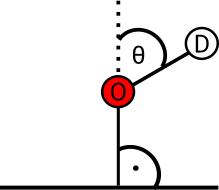
\includegraphics[width=2cm]{figures/11-20/ODangle.png}} \\\hline
  10 &2731 (44), 2694 (36) &2785 (26), 1711 (61) &2692 (41), 2689 (54)& \\
  15 &2728 (44), 2695 (36) &2783 (24), 1812 (60) &2711 (34), 2656 (60)& \\
  20 &2729 (44), 2694 (35) &2783 (24), 1838 (60) &2715 (34), 2665 (58)& \\
  25 &2728 (44), 2696 (35) &2767 (59), 1750 (62) &2764 (29), 2724 (41)& \\\hline
  exp. & \multicolumn{3}{c}{2839, 2812, 2762}& \\
  \end{tabular} 
  \label{tab:freq_layers}
\end{table*}
\\\\
 Following this approach we expect six modes, for each of the three an OD$_{surf}$ and an OD$_{ads}$. In all cases the relationship between the two individual modes for each considered structure is portrayed by $\tilde{\nu}$(OD$_{ads}$)>$\tilde{\nu}$(OD$_{surf}$). This can be explained with the different reduced mass for both vibrations: The OD$_{surf}$ oscillator has a slightly larger reduced mass since the deuterium is bound directly to the surface, whereas the adsorbed OD group can act more as a quasi-free OD group \cite{Wirth2014}. All these vibrations are clearly localized on one of the OD groups, which suggests that the normal modes ansatz is reasonable.
\\
Of course, normal modes of all molecular and next neighbor dissociated structures from 10 to the 25 slab layer model were calculated, although as it was mentioned in section \ref{structure_search11-20} that the slab was already converged with 10 layers concerning OD stretch frequencies.
\\
\\
To consider the probability of observing these species, we calculated their respective Boltzmann weights $P_i$:
\begin{equation}\label{boltzmann-weight}
 P_i=e^{-G_i/(k_BT)}.
\end{equation}
With this analysis it is possible to show the relative population for different temperatures, given in Table \ref{tab:boltzmann-pop}. In the temperature range relevant for the experiments, it is shown that the population of the species inter-CUSa$\parallel$O-$\mu_2$ clearly dominates and furthermore that the population of inter-CUSb$\parallel$O-$\mu_2$ is very low, compared to the others.
\begin{table*}[th]
  \centering
 \caption{Boltzmann population $P$ relative to the most stable inter-CUSa$\parallel$O-$\mu_2$, calculated according to Equation \ref{boltzmann-weight} for $130$, $300$ and $400\,$K. Values are given for the 10-layer system.}
\vspace*{.2cm} 
 \begin{tabular}{l|ccc}
  & P$_{130K}$ & P$_{300K}$ & P$_{400K}$\\\hline
  inter-CUSa$\parallel$O-$\mu_2$ &1 &1 &1 \\
  CUSb$\parallel$O-$\mu_2$ & 1.4$\times 10^{-6}$& 6.1$\times 10^{-3}$& 3.2$\times 10^{-2}$\\
  inter-CUSb$\parallel$O-$\mu_2$ & 1.0$\times 10^{-15}$ & 1.2$\times 10^{-6}$ & 6.6$\times 10^{-5}$\\
  \end{tabular} 
  \label{tab:boltzmann-pop}
\end{table*}
\\
From the results for the frequencies of the three most stable structures (from Table \ref{tab:freq_layers}), one can see, that for all slab sizes, there are 4 relevant modes to be expected. One of them is noticeable lower in energy that is due to hydrogen bonding (OD surface vibration of CUSb$\parallel$O-$\mu_2$). Also the angle of the bonding vector with respect to the surface normal is very high (i.e. the bond is more in plain, values and schematic representation shown in Tab.~\ref{tab:freq_layers}) so that the expected intensity in experiment is remarkably lower and may be not visible in experiment because of the angle dependence of the intensity in VSF. 
\\
With this in mind, we are able to predict 3 peaks, which fits well to the experimental results of Yanhua Yue from FHI Berlin (see Figure \ref{abb:exp-sfg}). Comparing these results in absolute numbers is not very convincing as before in the literature, but relative numbers are in good agreement (see results for experiment and all different sized layer slabs in Table \ref{tab:rel_modes}).
\begin{table*}[!h]
\begin{center}
\caption{Wave number differences $\Delta \tilde{\nu}$ are given in [cm$^{-1}$]. $\Delta \tilde{\nu}_1$ depicts the difference between the surface OD group of the inter-CUSa$\parallel$O-$\mu_2$ species and the respective surface OD group on O-$\mu_2$ and  $\Delta \tilde{\nu}_2$ is the difference between the same surface OD group and the adsorbed OD group on CUSb from CUSb$\parallel$O-$\mu_2$.}
\begin{tabular}{ccc}
layers & $\Delta \tilde{\nu}_1$ &  $\Delta \tilde{\nu}_2$\\\hline
10  &37 &91 \\
15  &33 &88 \\
20  &35 &89 \\
25  &32 &71 \\\hline
exp.&50 &77 \\
  \end{tabular}
\label{tab:rel_modes}
\end{center}
\end{table*}
\\
\\
Two problems of this approach are, that we neglect anharmonicities, that are especially important for hydrogen bonded vibrations and also the absence of neighbor effects, that can be solved by computing higher coverage systems.
\\
The influence of higher coverage was examined for some systems already presented in section \ref{structure_search11-20}. The coverage differs from 2D$_2$O molecules per super cell to 4 and 12 water molecules which equals 1ML. Here the frequencies of the OD stretching modes are affected due to the neighbor adsorbates, for some structures more and for other less (e.g. the system with 2 inter-CUSa$\parallel$O-$\mu_2$).
\todo{compare modes of low coverage limit to spetra with higher coverage, ask Lu for more data of higher coverage.}
\\
The simulation of intensities was done both with dipole corrections and Born effective charges and is shown in Table \ref{tab:freq_lowcov_comp} as a comparison. \todo{show only high frequency part, comparing BEC and dipole, for the most stable configurations. These are only IR intensities in both cases, that can not be set equal to SFG intensities but can be a first hint.}
\begin{table}[!h]
\centering
\caption{Comparison of the intensities obtained from dipole corrected calculations and from the Born effective charges based approach.}
\begin{tabular}{c|cc}
&\multicolumn{2}{c}{Intensity [a.u.]}\\
& dip. & BEC \\\hline
\multirow{2}{4cm}{inter-CUSa||O-$ \mu_2$}& & \\
 & & \\
\multirow{2}{4cm}{CUSb||O-$ \mu_2$} & & \\
 & & \\
\multirow{2}{4cm}{inter-CUSb||O-$ \mu_2$}& & \\
 & & \\
\end{tabular}
\label{tab:freq_lowcov_comp}
\end{table}
\\
Frequencies for the low coverage limit were also calculated using the crystal code, that enables calculations with atomic centered bases and makes it possible to treat a real 2-D system without the need to calculate the repetition of the slab in z-direction, see also section \ref{crystal_calc}. With this code it is also possible to calculate hybrid functionals easily, here B3LYP. For both PBE and B3LYP, geometries of the most stable states were reoptimized starting from VASP optimized geometries and normal modes were calculated. Also anharmonicities for OH/OD bonds were calculated, these results are shown in comparison with VASP results in Table \ref{tab:freqs11-20crystal}. First, PBE results from both programs do not differ largely. Anharmonicities decrease the wavenumbers and lead to worse agreement to experiment and to VASP calculations. Data from B3LYP calculations show great agreement with experiment, although here, anharmonic corrections make the agreement worse, too. This effect can be caused by error cancellation. One has to mention, that here influence of the basis set is strong and larger basis sets were not feasible due to high computational costs.
 \begin{table}[!h]
  \centering
   \caption{Stretch wavenumbers for both of the OD groups at the (11\=20) surface for the 3 most stable species, calculated with atom centered basis functions with the program crystal. Frequencies were calculated at the B3LYP+D3 and PBE+D3 level of theory, optimized with the respective method. As a basis pob\_TZVP was used. The VASP results were obtained with a plane wave basis and PBD+D2 corrections.}
  \begin{tabular}{ccc|cc|c}
   & \multicolumn{2}{c}{PBE} & \multicolumn{2}{c}{B3LYP} &VASP result\\
  stretch & $\tilde{\nu}$ [cm$^{-1}$] &$\tilde{\nu}$+anharm [cm$^{-1}$] &$\tilde{\nu}$ [cm$^{-1}$] & $\tilde{\nu}$+anharm [cm$^{-1}$]&$\tilde{\nu}$ [cm$^{-1}$]\\\hline
  iCa2: OD$_{\textrm{surf}}$ &2682 &2599 &2773 &2695 & 2694\\
  iCa2: OD$_{\textrm{ads}}$  &2728 &2644 &2811 &2729 & 2731\\
  Cb2: OD$_{\textrm{surf}}$  &1658 &1310 &2019 &1722 & 1711\\
  Cb2: OD$_{\textrm{ads}}$   &2769 &2687 &2843 &2765 & 2785\\
  iCb2: OD$_{\textrm{surf}}$ &2657 &2595 &2778 &2694 & 2689\\
  iCb2: OD$_{\textrm{ads}}$  &2688 &2569 &2777 &2689 & 2692\\
  \end{tabular}
  \label{tab:freqs11-20crystal}
  \end{table}

\subsubsection{Lattice Vibrations}\label{phonons}
For the phonons as a first test the same normal modes analyses were checked to get a first impression into how the spectra can look like. But for a better description we need to consider more layers of the bulk in order to get more reliable results. From an experimental point of view it is suggested that SFG spectra can give insight into \todo{x} layers of the bulk \todo{ask Lu!}. Therefore we did calculations for the most stable adsorption geometries for more layered systems, going up to $6\times 5=30$ layers (with 5 being the number of layers in the unit cell in z direction), both for the clean surface and for the adsorbate covered surface, here we used again optimized geometries of the most stable structures. For adsorption energies for different slab sizes see Table \ref{tab:eads_layers}. These results are also shown with intensities calculated from dipole corrected normal mode analyses. The additional geometries with more layers do not differ strongly from the 10 layer ones that were presented in section \ref{structure_search11-20}.
\\
\todo{compare clean surface for different sizes, iCa2, Cb2 and iCb2 for all slab sizes. Normal modes may not be a perfect description of these deeply delocalized vibrations.. intensities for lattice vibrations from BEC and dip..
\\
Wait for Boss to correct the paper draft!}

\subsection{Velocity-Velocity Autocorrelation Function}\label{vvacf}
\todo{Extract vel vel autocorrelation function from MD at $300\,$K from most stable structures (inter-CUSa||O-$\mu_2$, CUSb||O-$\mu_2$ and inter-CUSb||O-$\mu_2$), with Fourier transformation converted to VDOS spectrum. It also is possible to separate modes from water layers from bulk phonons. Not really important if you don't use hydroxylated surface with a higher water coverage? So for Giacomo's system it makes sense, but here it is unnecessary.
\\
Totally different ansatz, no freq analysis, no harmonic approximation, but \textit{ab initio} MD trajectories at 300K, starting from optimized minimum structures. trajectory duration of 1-a few ps. calculating vac, fourier transform gives power spectra, no real IR, but still one can relate to intensities. results for trajectories.}

\section{Desorption Process}
\todo{not sure if this is worth a whole chapter..}
\\
Not only the reactions at the surface are of interest but also the process of adsorption and desorption were studied. The experimentalist's method to do so is TPD (thermal desorption spectroscopy, see Appendix). It is possible to measure the bond strength of the adsorbates, depending on the temperature they can be found to desorb. \todo{The sample was flashed to $400\,$K to get rid of impurities. The results showed two peaks, one beneath $400\,$K and one above SIND DIESE DATEN NOCH AKTUELL?} This peak beneath $400\,$K should not be visible, since the sample was heated to that temperature and all adsorbates that are released beneath this temperature should not be there any more. The only plausible explanation to this is, that there are reactions, that fill this species up and so the desorption can still be from this species.
\\
To interpret these results, one has to think of a possible reaction scheme from the most stable adsorption sites via the molecular state leading to the gas phase molecule.
\\
Here the most stable inter-CUSa$\parallel$O-$\mu_2$, CUSb$\parallel$O-$\mu_2$ and inter-CUSb$\parallel$O-$\mu_2$ and their reactions
\\
calculation with NEB was not done, instead geometry optimization for a water molecule above 3 interesting points on the potential energy surface (above inter-CUSa, CUSb and inter-CUSb).
\begin{verbatim}
  /und/sophia/bigger-cell_newcrystalcut/2x2cell/2layers/gasphase-physisorbed
\end{verbatim}

It was also tried to study the adsorption/desorption process (not with NEB), since there was no minimum structure in the gas phase nor physisorbed state. But from a single water molecule above the surface, geometry optimizations were done. Three structures were tested above inter-CUSa, CUSb and inter-CUSb. The energy profile is smooth from any tested point on the potential energy surface above the alumina surface towards the adsorbed water system without showing a barrier but indeed both showing an intermittend molecularly adsorbed structure.
\\
As mentioned before the experimentalists measure TPD in order to understand the adsorption strength and possible exchange reactions. We tried to simulate the desorption process using the following scheme: take the water in the gas phase + the clean surface as the standard. In the thermal equilibrium, the water should be equally distributed to Boltzman's distribution in the most stable structures. From this situation the water can recombine to the molecularly adsorbed water. The recombined water then can desorb to the gas phase. Since the spectrum is measured in ultra high vacuum it can be assumed that all the water that has left the surface will not return to the system, because it is dragged out of the equilibrium by the vacuum pumps.
Applying the reaction rates of the corresponding reactions in a kinetic Monte Carlo approach leads to 
{\color{red} Redo these calculations? I don't think that this is worth the effort..}

{\color{green} does it make sense to bring this cause there is no good agreement between our theory and the experimental findings..? The NEB didn't lead to anything since there is no minimum (just try a NEB??), optimization doesn't show any kind of barrier and just modelling the desorption from the rates is not good enough, sonce the rate for Cb2-Cb is too small to.}

%%%%%%%%%%%%%%%%%%%%%%%%%%%%%%%%%%%%%%%%%%%%%%%%%%%%%%%%%%%%%%%%%%%%%%%%%%%%%%%%%%%%%%%%%%%%%%%%%%%%%%%%%%%%%%%%%%%%%%%%%%%%%%%%%%%%%%%%%%%%%%%%%%%%%%%%%%%%%%%%%%%%%%%%%%%%%%%%%%%%%%%%%%%%%%%%%%%%%%%%%%%%%%%%%%%%%
%%%%%%%%%%%%%%%%%%%%%%%%%%%%%%%%%%%%%%%%%%%%%%%%%%%%%%%%%%%%%%%%%%%%%%%%%%%%%%%%%%%%%%%%%%%%%%%%%%%%%%%%%%%%%%%%%%%%%%%%%%%%%%%%%%%%%%%%%%%%%%%%%%%%%%%%%%%%%%%%%%%%%%%%%%%%%%%%%%%%%%%%%%%%%%%%%%%%%%%%%%%%%%%%%%%%%

\chapter{Water on $\upalpha$-Al$_2$O$_3$(0001)}
The (0001) surface is the most stable surface site of alumina under UHV conditions, and was subject of several studies so far. Both experimental and theoretical studies discovered characteristics and specialties of this crystal cut. In our workgroup previous work was done concerning the stability of low limit water coverage and their vibrational spectroscopic behaviour, reaction pathways between these stable minima, but also studying higher water coverages and hydroxylated surface systems\cite{WirthJPCC2012,Wirth2014,Wirth2015}.
\\
In this work, the focus lies more on two topics:
\\
(i) Understanding the processes of a water molecule (D$_2$O) being shot at the surface with a molecular beam source with the help of \textit{ab initio} Molecular Dynamics and
\\
(ii) The improvement of reaction rates with different methods beyond GGA functionals (as PBE).
\\
First, the surface and the most stable adsorption patterns are introduced (section \ref{sec_0001surf}), followed by the results for the molecular beam scattering (section \ref{sec_0001AIMD}) and last the improvements for the reaction rates (see section \ref{sec_rates}).
	
\section{Surface Model and Static Calculations}\label{sec_0001surf}
The most stable surface cut is a stochiometric, Al terminated one, and in contrast to the (11\=20) surface there is only one type of Al-CUS atom, which is a reactive Lewis-acid site. Also, all oxygen atoms are threefold coordinated, that leads to a topography that is not as complex as for the higher indexed surfaces. We applied here a $2\times 2$ supercell with vectors that were optimized from the bulk structure vectors (previous work of J. Wirth\cite{WirthJPCC2012}). The surface slab consists of 9 atomic layers, that is three repeating units in z direction of the type Al-O$_3$-Al..., with the top 5 layers being allowed to relax during optimization and AIMD and the lowest 4 layers being fixed to bulk values, see Figure \ref{abb:surf_0001}. The unit cell vectors in there are equal to $\uline{a}=\uline{b}=9.66\,$\AA  ~and a $60$\textdegree{} angle between them. The $\uline{c}$-vector of the slab model is $31.4\,$\AA~ long, hence the vacuum gap between two slabs in this direction is $26.4\,$\AA.
\\
The stability, vibrations and reactivity of one water  molecule per $2\times 2$ supercell were already studied by Dr. Jonas Wirth. As it was published in \cite{WirthJPCC2012}, there is one molecular minimum on top of a CUS atom and 3 dissociated states (see Figure \ref{abb:0001_ads}): the next neighboring 1-2 dissociated state, the 1-4 dissociated structure with the Hydrogen atom being one position further and the 1-4$^\prime$ that is the configuration with the greatest distance that is possible for this slab size. From these, the 1-2 dissociated species is the most stable one and the 1-4$^\prime$ is the least stable one. For the stability of the molecular and the 1-4 dissociated species, the situation is more controversial in the literature. In our periodic DFT studies with VASP, it lies between the previously mentioned ones, depending on the exact method employed, for PBE+D2 the molecular adsorbed species is more stable than 1-4, for PW91+D2 the 1-4 dissociated is more stable, whereas PW91 without dispersion corrections gives the same adsorption energy for both species (the values for the adsorption energy are calculated analogously to the (11\=20) surface cut, see eq.~\ref{eq:Eads}).
Calculations with an atom centered basis instead of plane waves with the crystal code show, that for most basis sets the molecular species is more stable and for others, they are both equal in adsorption energy.
\\
Of course, there are reactions linking these minima, dissociation, OH- and H-diffusion were studied, as well as rotation of an OH group and molecular water diffusion from CUS to CUS. The latter two do not play a crucial role in this work, especially the CUS to CUS diffusion of molecular water is very improbable due to the slow reaction rate. Adsorption energies and reaction rates that are important for this work are shown in Table \ref{tab:0001_eads+rates}, these results were obtained by J. Wirth and were unpublished.
 \begin{table}[!h]
  \centering
   \caption{Adsorption energies for the stable minima (left part) and reaction rate constants $k$ in s$^{-1}$ at $300\,$K with corresponding barrier heigths $\Delta E^\ddagger$/$\Delta G^\ddagger_\textrm{300K}$ in eV for the processes connecting these minima (right part). Here the upper two line shows the reaction in the direction given in the name and the lower two line gives the back reaction's rates constants and barriers. All values were calculated with PBE including D2 dispersion corrections and are unpublished work of J. Wirth.}
  \begin{tabular}{cccc|ccccc}
   \multicolumn{4}{c}{E$_\textrm{ads}$ [eV]}&\multicolumn{5}{c}{k$_\textrm{300K}$ [s$^{-1}$]}\\
  mol &1-2 &1-4 &1-4$^\prime$  &diss-1-2            & diss-1-4            & diff-2-4         & diff-2-4$^\prime$ & diff-4-4$^\prime$\\
  -1.31 & -1.69 & -1.30 & -1.21&8.0$\times 10^{10}$  & 2.8$\times 10^{10}$ & 2.7$\times 10^1$  & 3.8$\times 10^1$  & 7.1$\times 10^5$ \\
   & & & &0.13/0.11 & 0.19/0.14& 0.82/0.68&0.81/0.67 &  0.61/0.41\\\hline
   & & &                       &2.3$\times 10^4$    & 2.7$\times 10^{10}$ & 9.1$\times 10^7$ & 3.1$\times 10^9$ & 1.7$\times 10^7$ \\
   & & & & 0.50/0.50 & 0.19/0.14 & 0.44/0.29 & 0.33/0.20 & 0.51/0.33\\
    \end{tabular}
  \label{tab:0001_eads+rates}
  \end{table}

The adsorption process itself was studied, by starting from the molecular minimum, gradually doing optimizations with greater O-surface distance and letting everything relax except for the c-coordinate of the water-oxygen atom. This calculations gives an energy profile for the adsorption/desorption but no barrier could be found (see Figure \ref{abb:0001_desorption}), so the underlying adsorption process is thought to be barrierless.
  \begin{figure}[!ht]
   \centering
   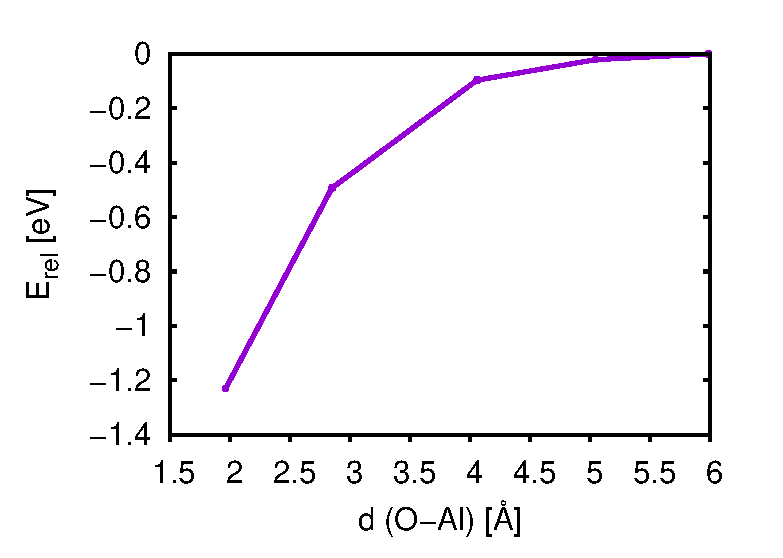
\includegraphics[width=0.45\textwidth]{figures/0001/mol_ads_barrier.eps}
   \caption{Energy profile of the adsorption process, relative to the energy of the system with a distance of $5.98\,$\AA. The d(O-Al) denotes the distance between the oxygen atom of the water and the Al-CUS where the water is/was adsorbed molecularly. %/und/sophia/0001_mol_ads_barrier/
   }
   \label{abb:0001_desorption}
  \end{figure}

  
  
\begin{figure}[!ht]
 \centering
\subfigure[(0001), top view]{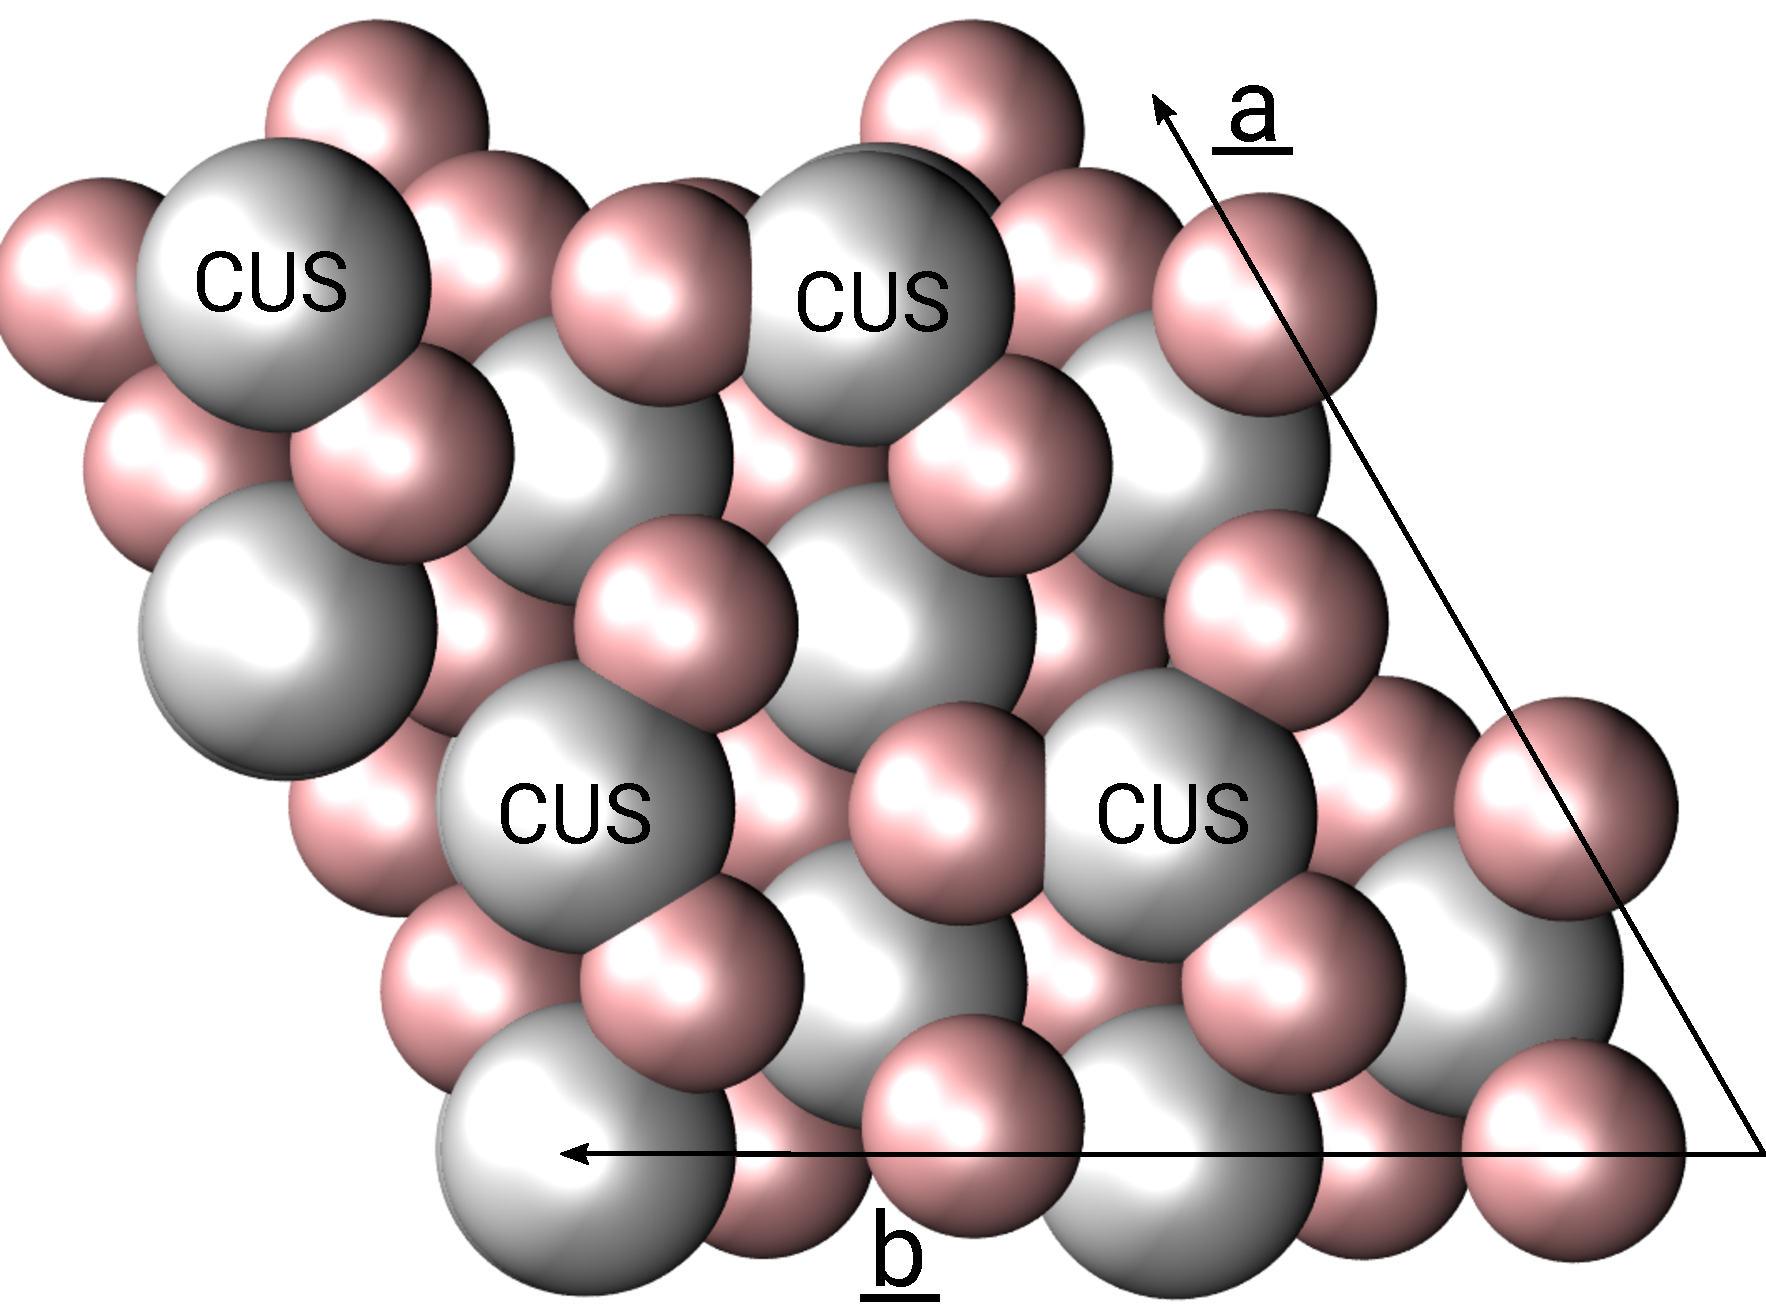
\includegraphics[width=0.45\textwidth]{figures/0001/surf_0K_axes.pdf}}
 \quad\quad
 \subfigure[(0001), side view]{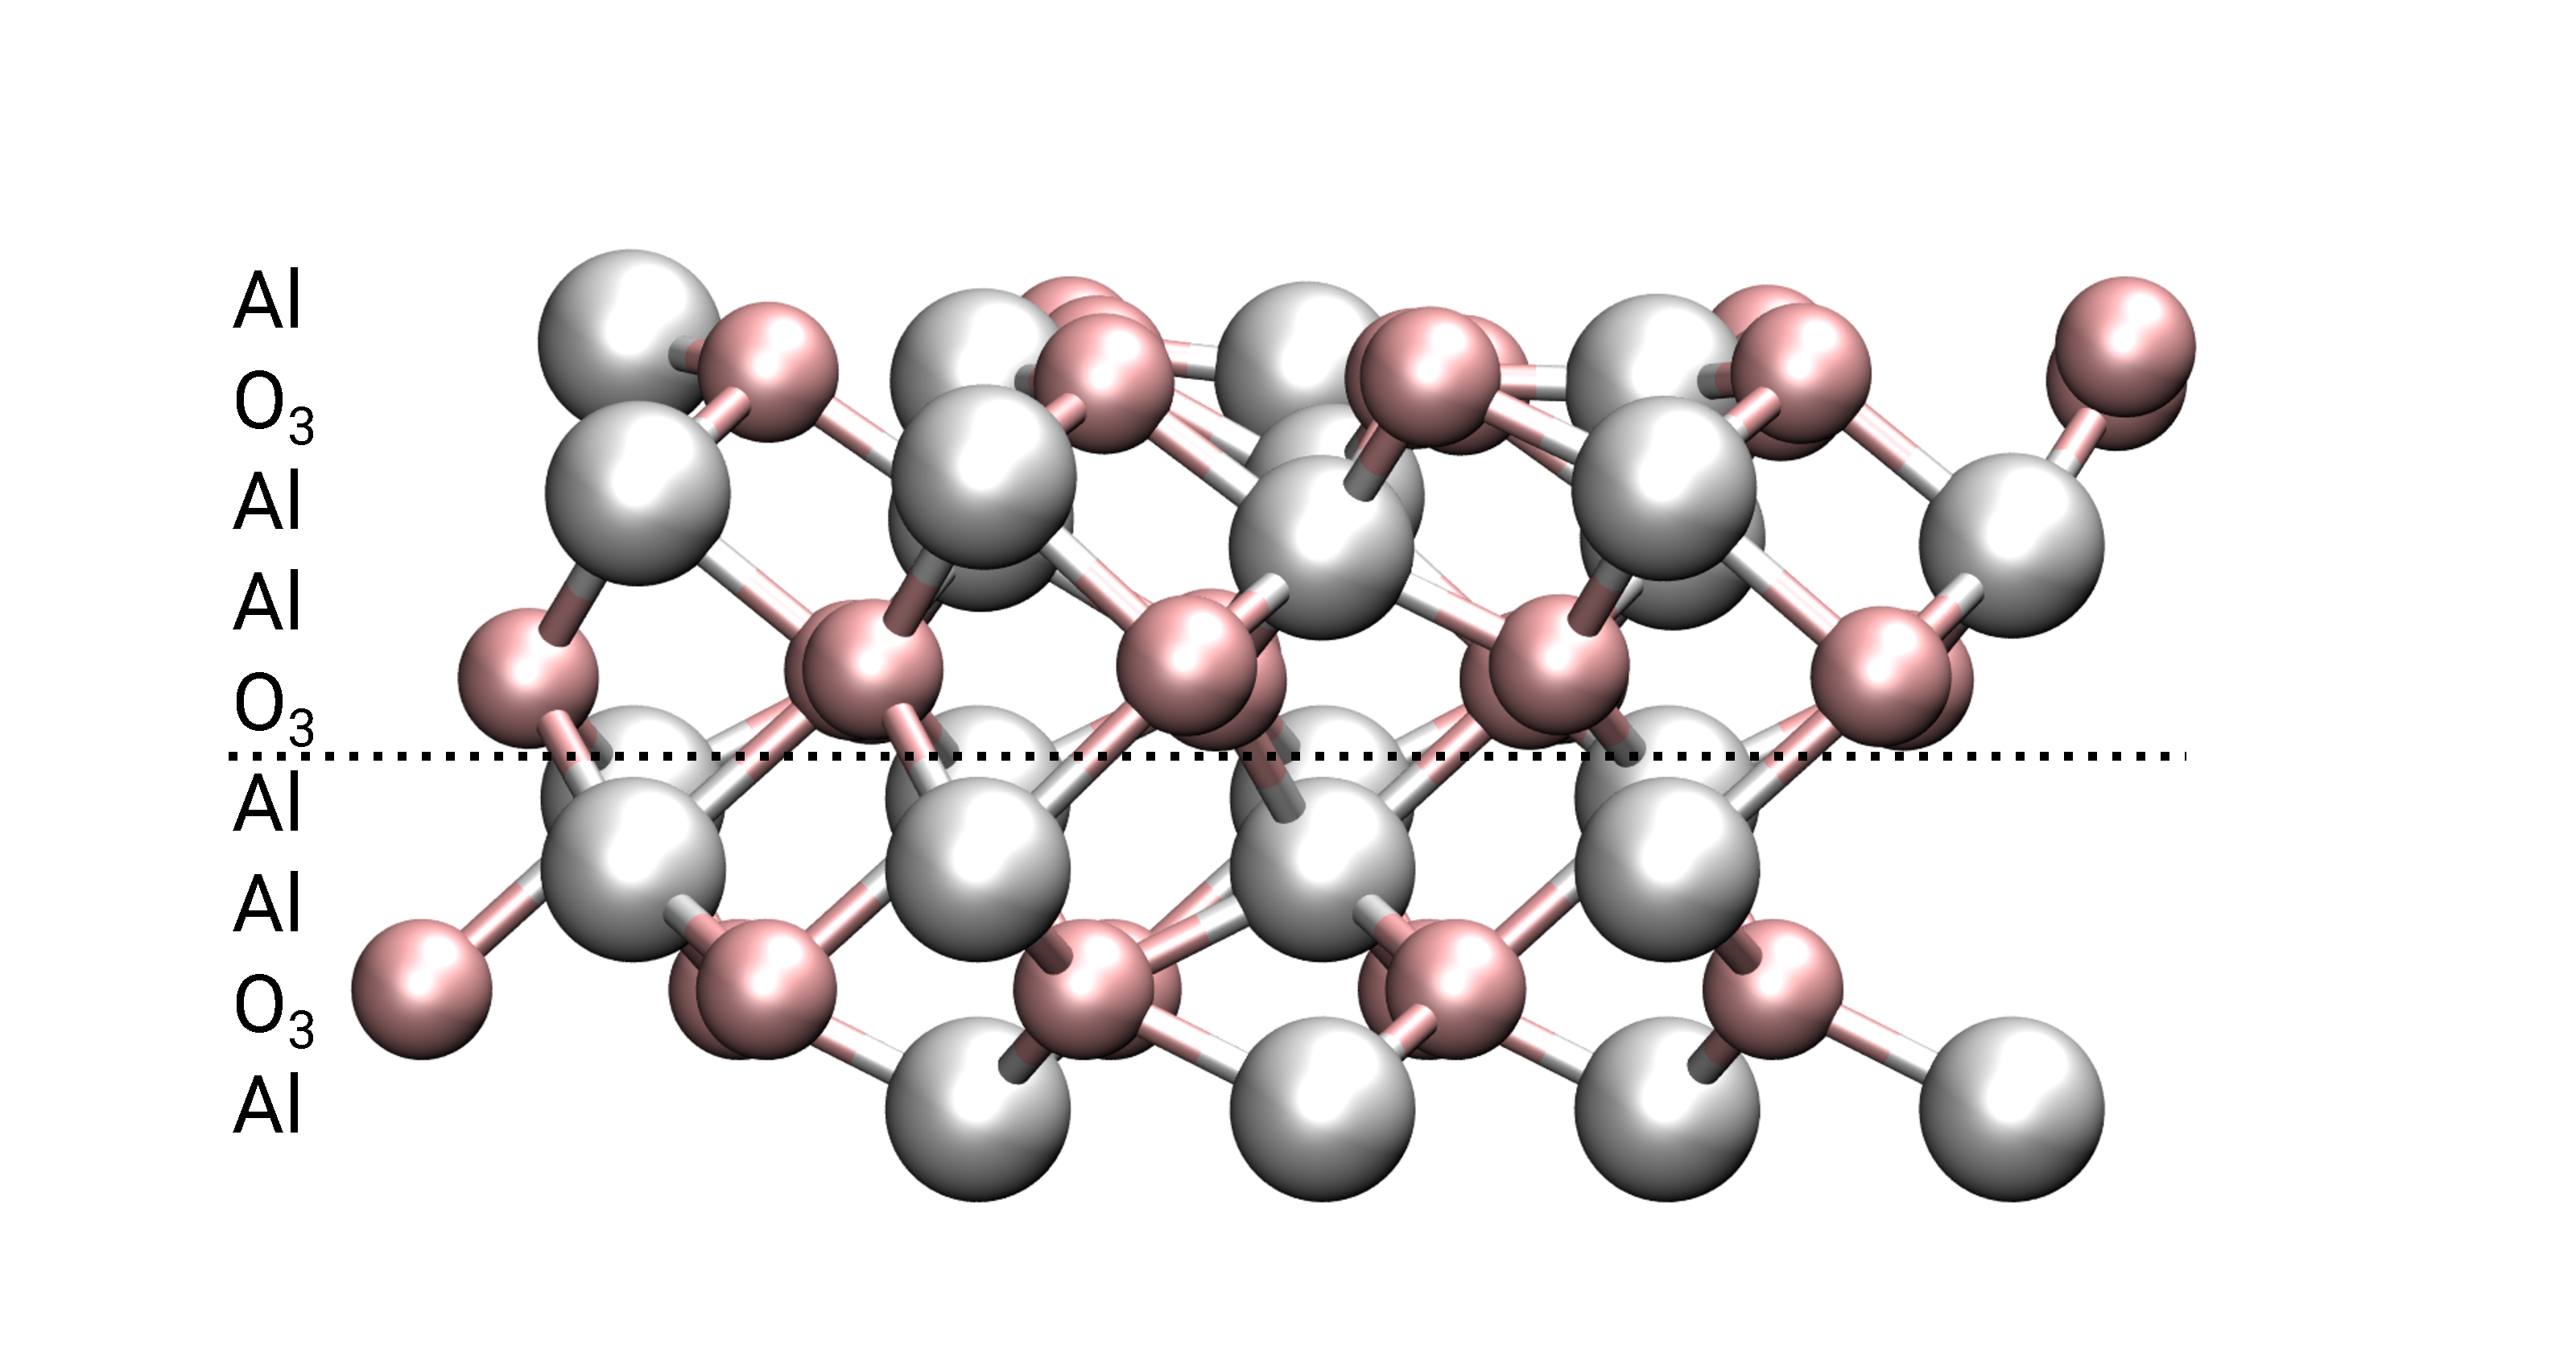
\includegraphics[width=0.45\textwidth]{figures/0001/surf_0K-side.pdf}}
 \caption{Surface model of the (0001), the most stable surface cur under UHV conditions. The top view (a) shows 4 Al CUS atoms, that are surrounded by three threefold coordianted surface oxygen atoms. (b) reveals the Al terminated surface cut in detail with the atomic layers.}
        \label{abb:surf_0001}
 \end{figure}

 \begin{figure*} [!ht]
\centering
\subfigure[mol]{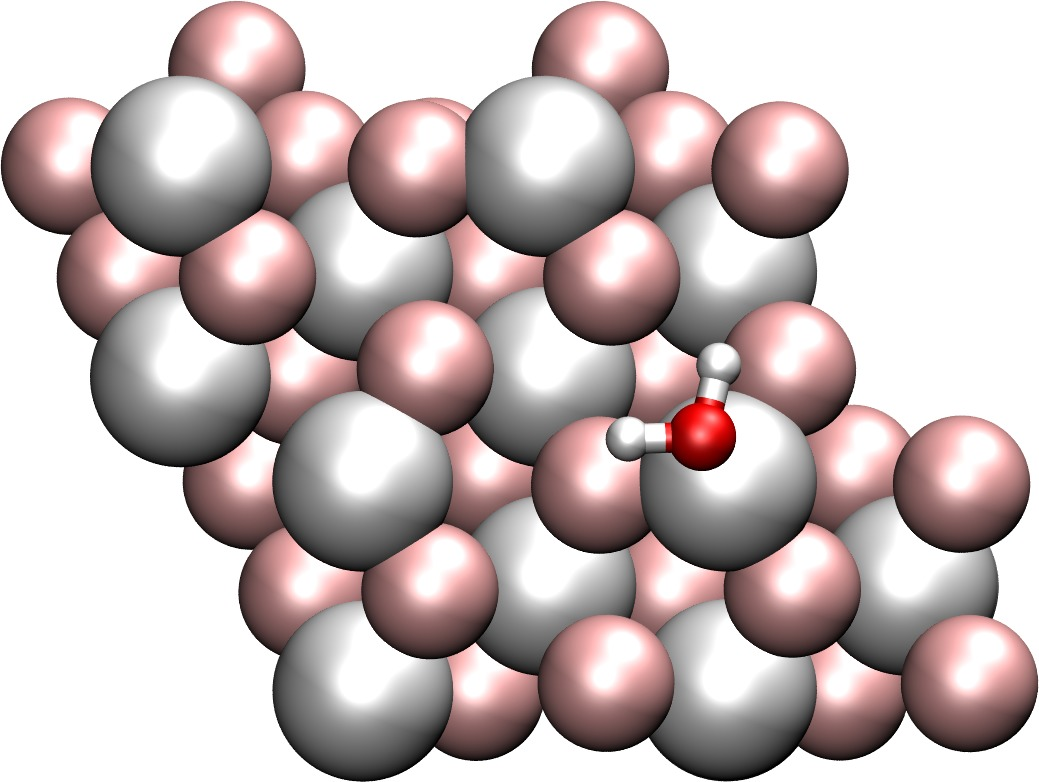
\includegraphics[width=0.4\textwidth]{figures/0001/0001_mol_top.jpg}}
         \quad
\subfigure[1-2]{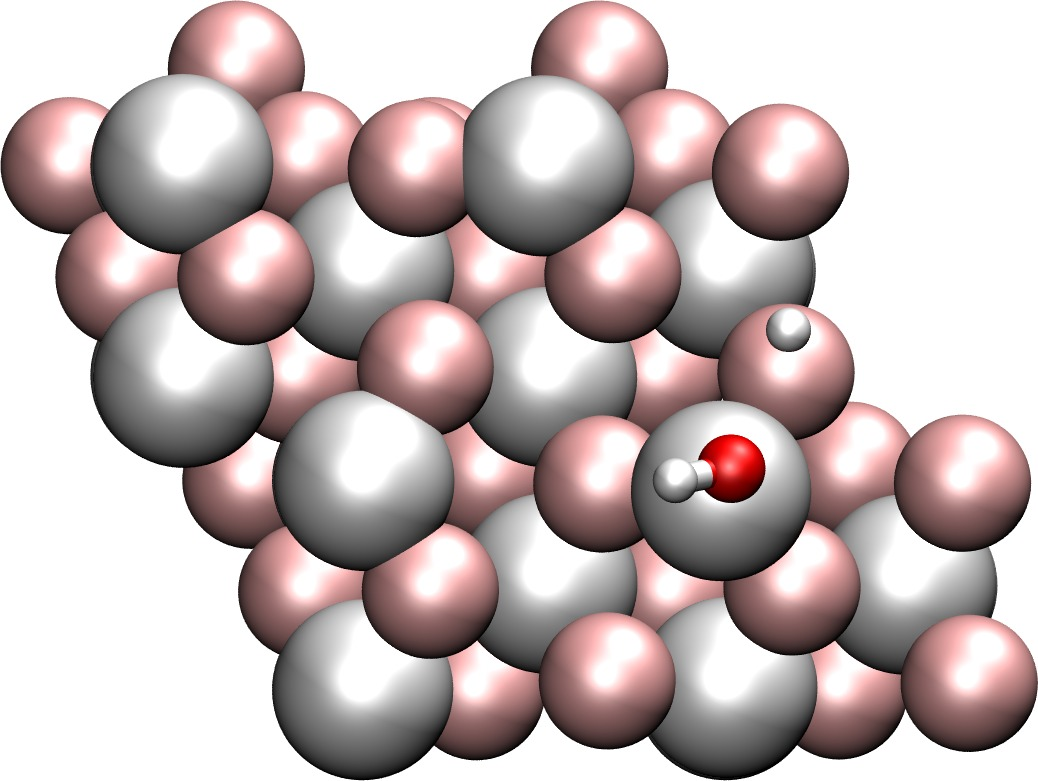
\includegraphics[width=.4\textwidth]{figures/0001/0001_1-2-diss_top.jpg}}
 \quad
\subfigure[1-4]{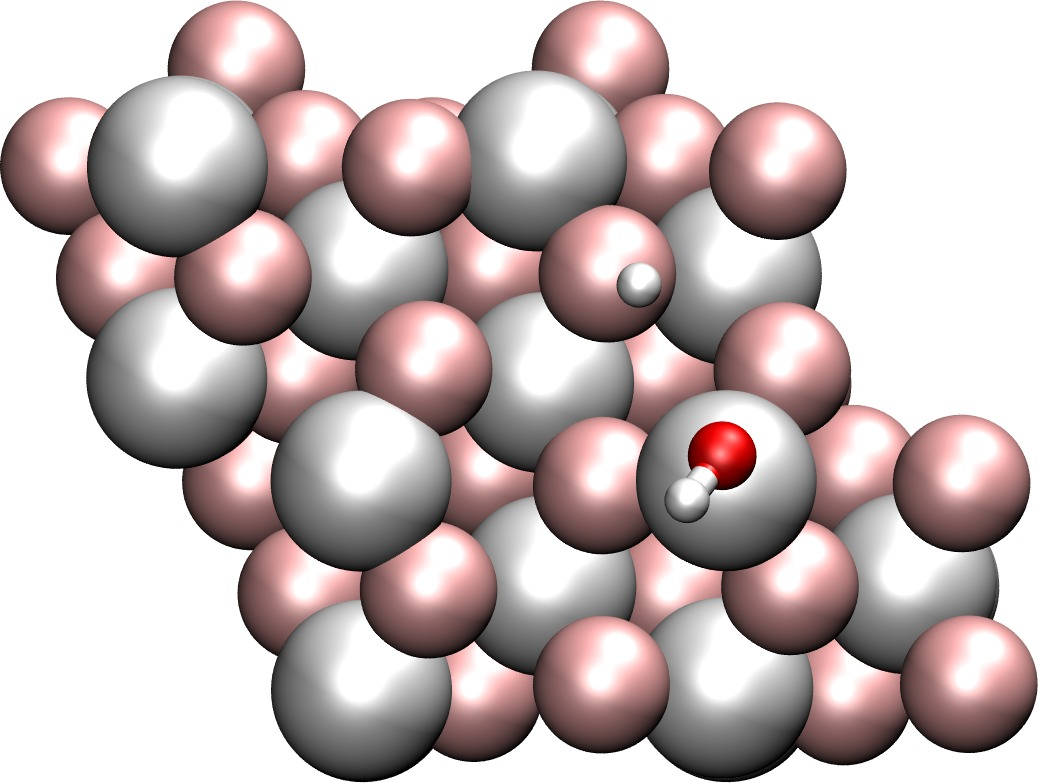
\includegraphics[width=.4\textwidth]{figures/0001/0001_1-4-diss_top.jpg}}
 \quad
\subfigure[1-4$^\prime$]{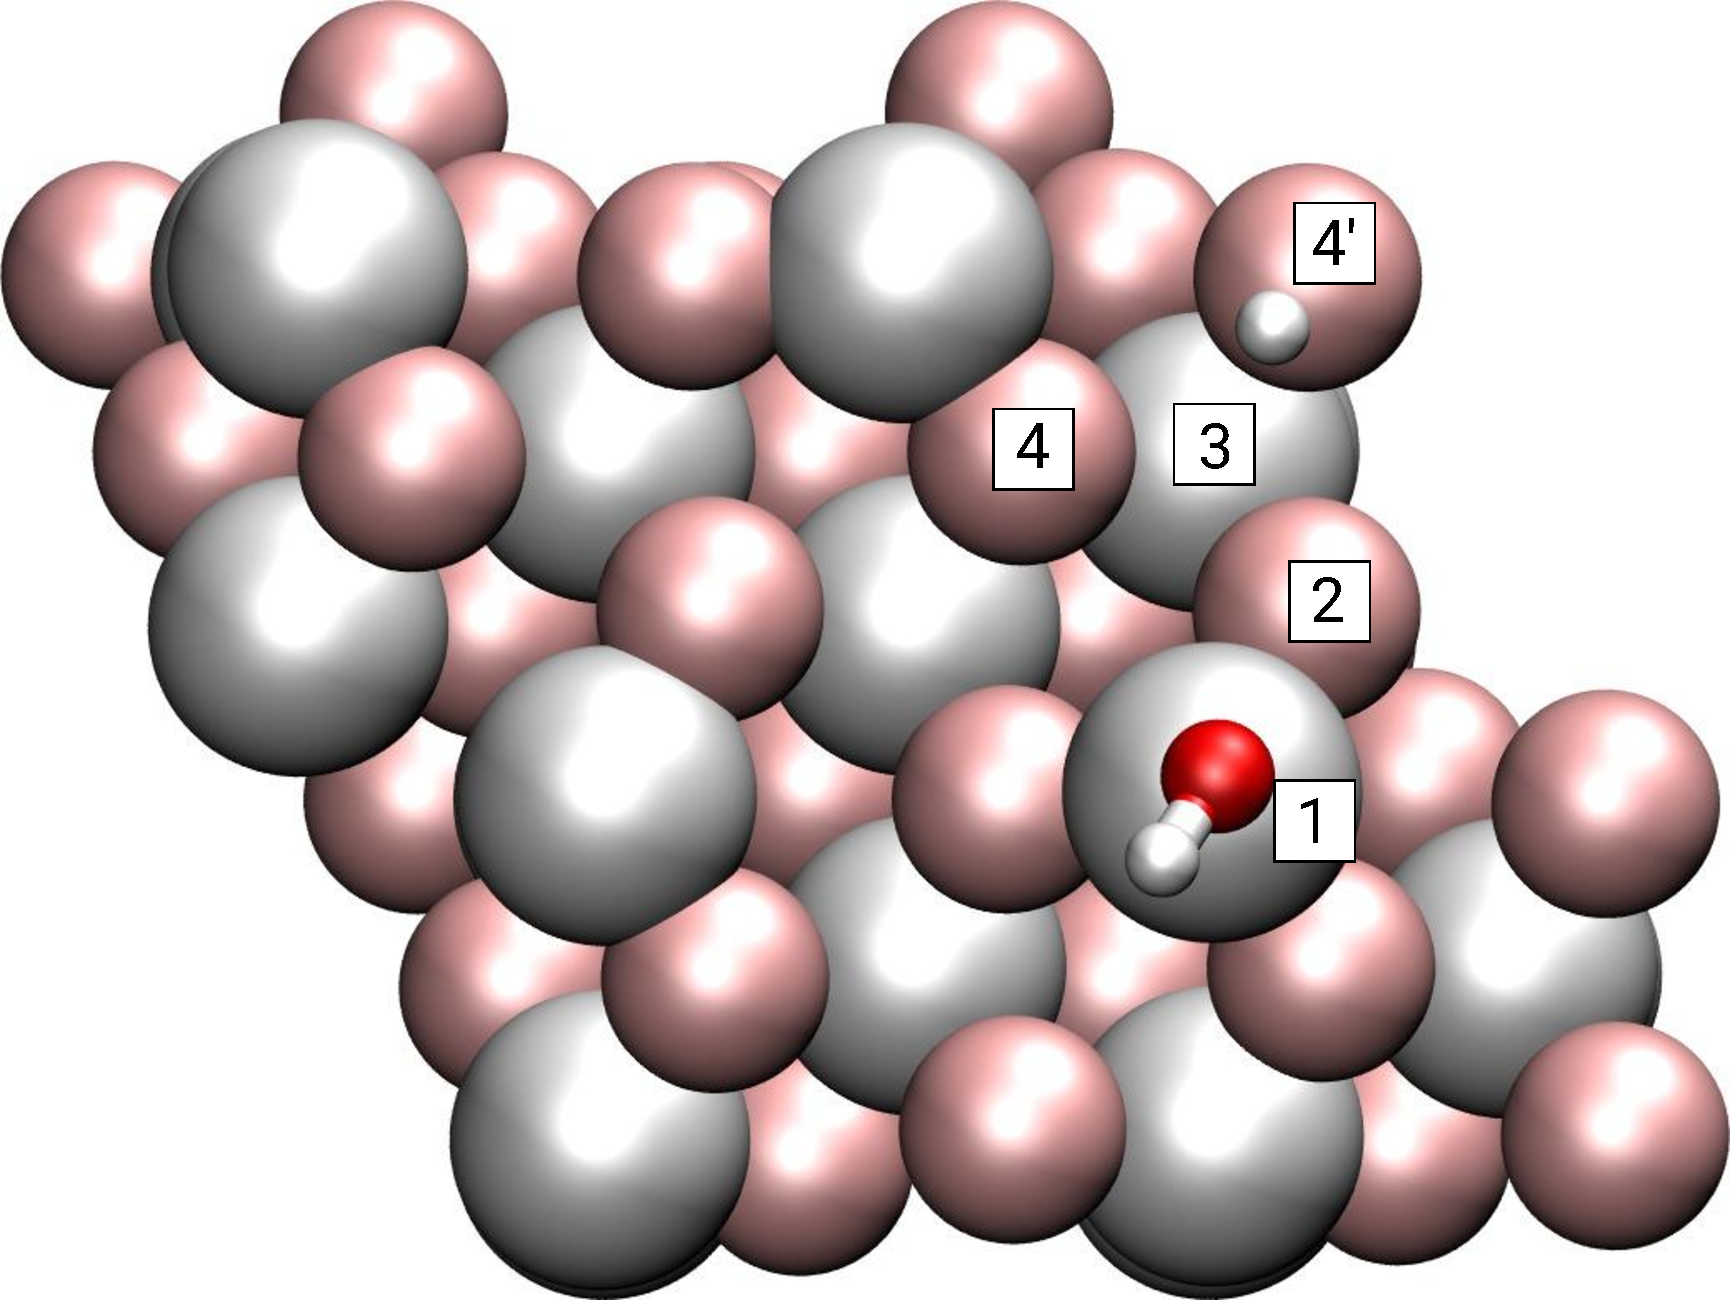
\includegraphics[width=.4\textwidth]{figures/0001/0001_1-4p-diss_top_label.pdf}}
\caption{Adsorption geometries of the molecular and the three dissociated species. Adsorption energies for these species can be found in Table \ref{tab:0001_eads+rates}.}
       \label{abb:0001_ads}
\end{figure*}
\section{AIMD for MBS Process}\label{sec_0001AIMD}
\todo{Hass. heavy water (D$_2$O) was used instead of H$_2$O to better compare with existing MBS experiments by R. K. Campen.
\\
Should I put the data in the appendix?}
\\
Molecular beam experiments have shown recently that water is able to adsorb both molecularly
 and dissociatively on an $\alpha$-Al$_{\text{2}}$O$_{\text{3}}$(0001) surface.
 The results show an enhanced dissociation probability compared to ``pinhole dosing'', which may be referred to as adsorption 
 under thermal equilibrium conditions.
 However, precise mechanistics of the ongoing reactions 
 and their relative probabilities are not known.
 In this work \textit{Ab Initio} Molecular Dynamics calculations
 were conducted to unravel this process.
 In these simulations water collides with the $\upalpha$-Al$_{\text{2}}$O$_{\text{3}}$(0001) surface.
 
%%%%%%%%%%OLD VERSION%%%%%%%%%%%%%%%%%
% Hass et. al. discussed the idea whether water will adsorb molecularly first and then dissociate or if direct dissociation upon adsorption is possible. To tackle this question for the experimental technique of the molecular beam source, we apply both microcanonical and canonical \textit{ab initio} MD to simulate water in the beam approaching the surface. Interestingly, these experiments also show a higher disociation probability compared to pinhole dosing, that leads to an ensemble in thermal equilibrium, whereas MBS leads to a non-equilibrium situation. We start in the low coverage limit by letting one single, rigid molecule approach the $2\times 2$ supercell with only a linear momentum towards the surface. We later on continue with different approaches to more realistic beams and to more realistic surface situations. In the beam regime we probe water clusters, namely pre-optimized %(H$_2$O)$_2$ and
% (H$_2$O)$_4$ cluster, which is shot onto the surface. Another improvement to the beam lies in exciting the molecule either vibrationally and/or rotationally. These excitations were chosen from a normal mode analysis and the resulting stretch and bending modes.
% \\
% For improving the surface we first use a preequilibrated surface at $300\,$K, but also go to a surface situation in which already one water molecule is adsorbed. To pay attention to the equilibrium situation we considered a molecular preadsorbed water molecule,  the most stable 1-2 dissociated state as well as the 1-4 dissociated structure.
% \\
% We could show that water can both dissociate upon direct contact with the surface and also dissocioate after being adsorbed molecularly first and then after a time have enough energy to dissociate. This is mostly to the 1-2 dissociated state but also 1-4 and more surprisingly 1-4$^\prime$. It seems that the rotation of the water molecule before hitting the surface is crucial for direct dissociation. This energy can also be delivered by the heated surface, it has more energy in form of vibration, in this case prolongation of the respective OH bond and can therefore lead to dissociation. On the other hand hitting the surface directly on top of a CUS atoms was shown to lead mainly to reflection of the molecule, because the energy of the incoming molecule could not be absorbed by the surface.
% \\
% Trajectories with the vibrationally excited modes led to statistically higher levels of dissociation. Also temperature effects of the thermalized trajectories (canonical MD) seem to have a positive influence on the dissociation.
\subsection{Beam Model}
For the understanding of a Molecular Beam source experiment, the introduction of a beam is an essential part of the model. However, it was not possible to compute a fully realistic beam that was statistically converged, which would require wide knowledge about energy and velocity distributions and a systematic high dimensional sampling, that is not feasible with the computational power available at the moment. Instead as a first approach, a single, rigid water (D$_2$O) molecule (initial parameters are $d_{OD}=0.97$\AA~ and bond angle of $104.5$\textdegree) was sent perpendicularly from a center of mass position from a distance of $4\,$\AA~ onto the surface, in agreement with the experiment. Having these degrees of freedom excluded, from the 9 degrees of freedom, six are still left (see Figures \ref{abb:initial_parameters}, \ref{abb:impact_points} and Table \ref{tab:orientations}): two for the impact site [$a_0$,$b_0$] as it is given relative to the super cell vectors $\uline{a}$ and $\uline{b}$, three Euler angles $\alpha$, $\beta$ and $\gamma$ for the rotational orientation of the molecule with respect to the surface and the kinetic energy E$_\textrm{kin}$ that gives the molecule a momentum towards the surface, solely as translational motion, no vibration or rotation included. These parameters are varied systematically to gain insight into the process.
\\
As was mentioned before, the barriers can be high (and corresponding rates low), especially for the H-diffusion reactions, but the adsorption process itself is barrierless, and additionally the incoming water molecule has kinetic energy so that processes, that are slow at room temperature otherwise, can be speeded up.
\\
Further improvements of this simplest model are made in subsections \ref{clusters} and \ref{preex}, that address clustering and rotational and vibrational excited water, respectively. Further details are given there.

\begin{figure}[!ht]
 \centering
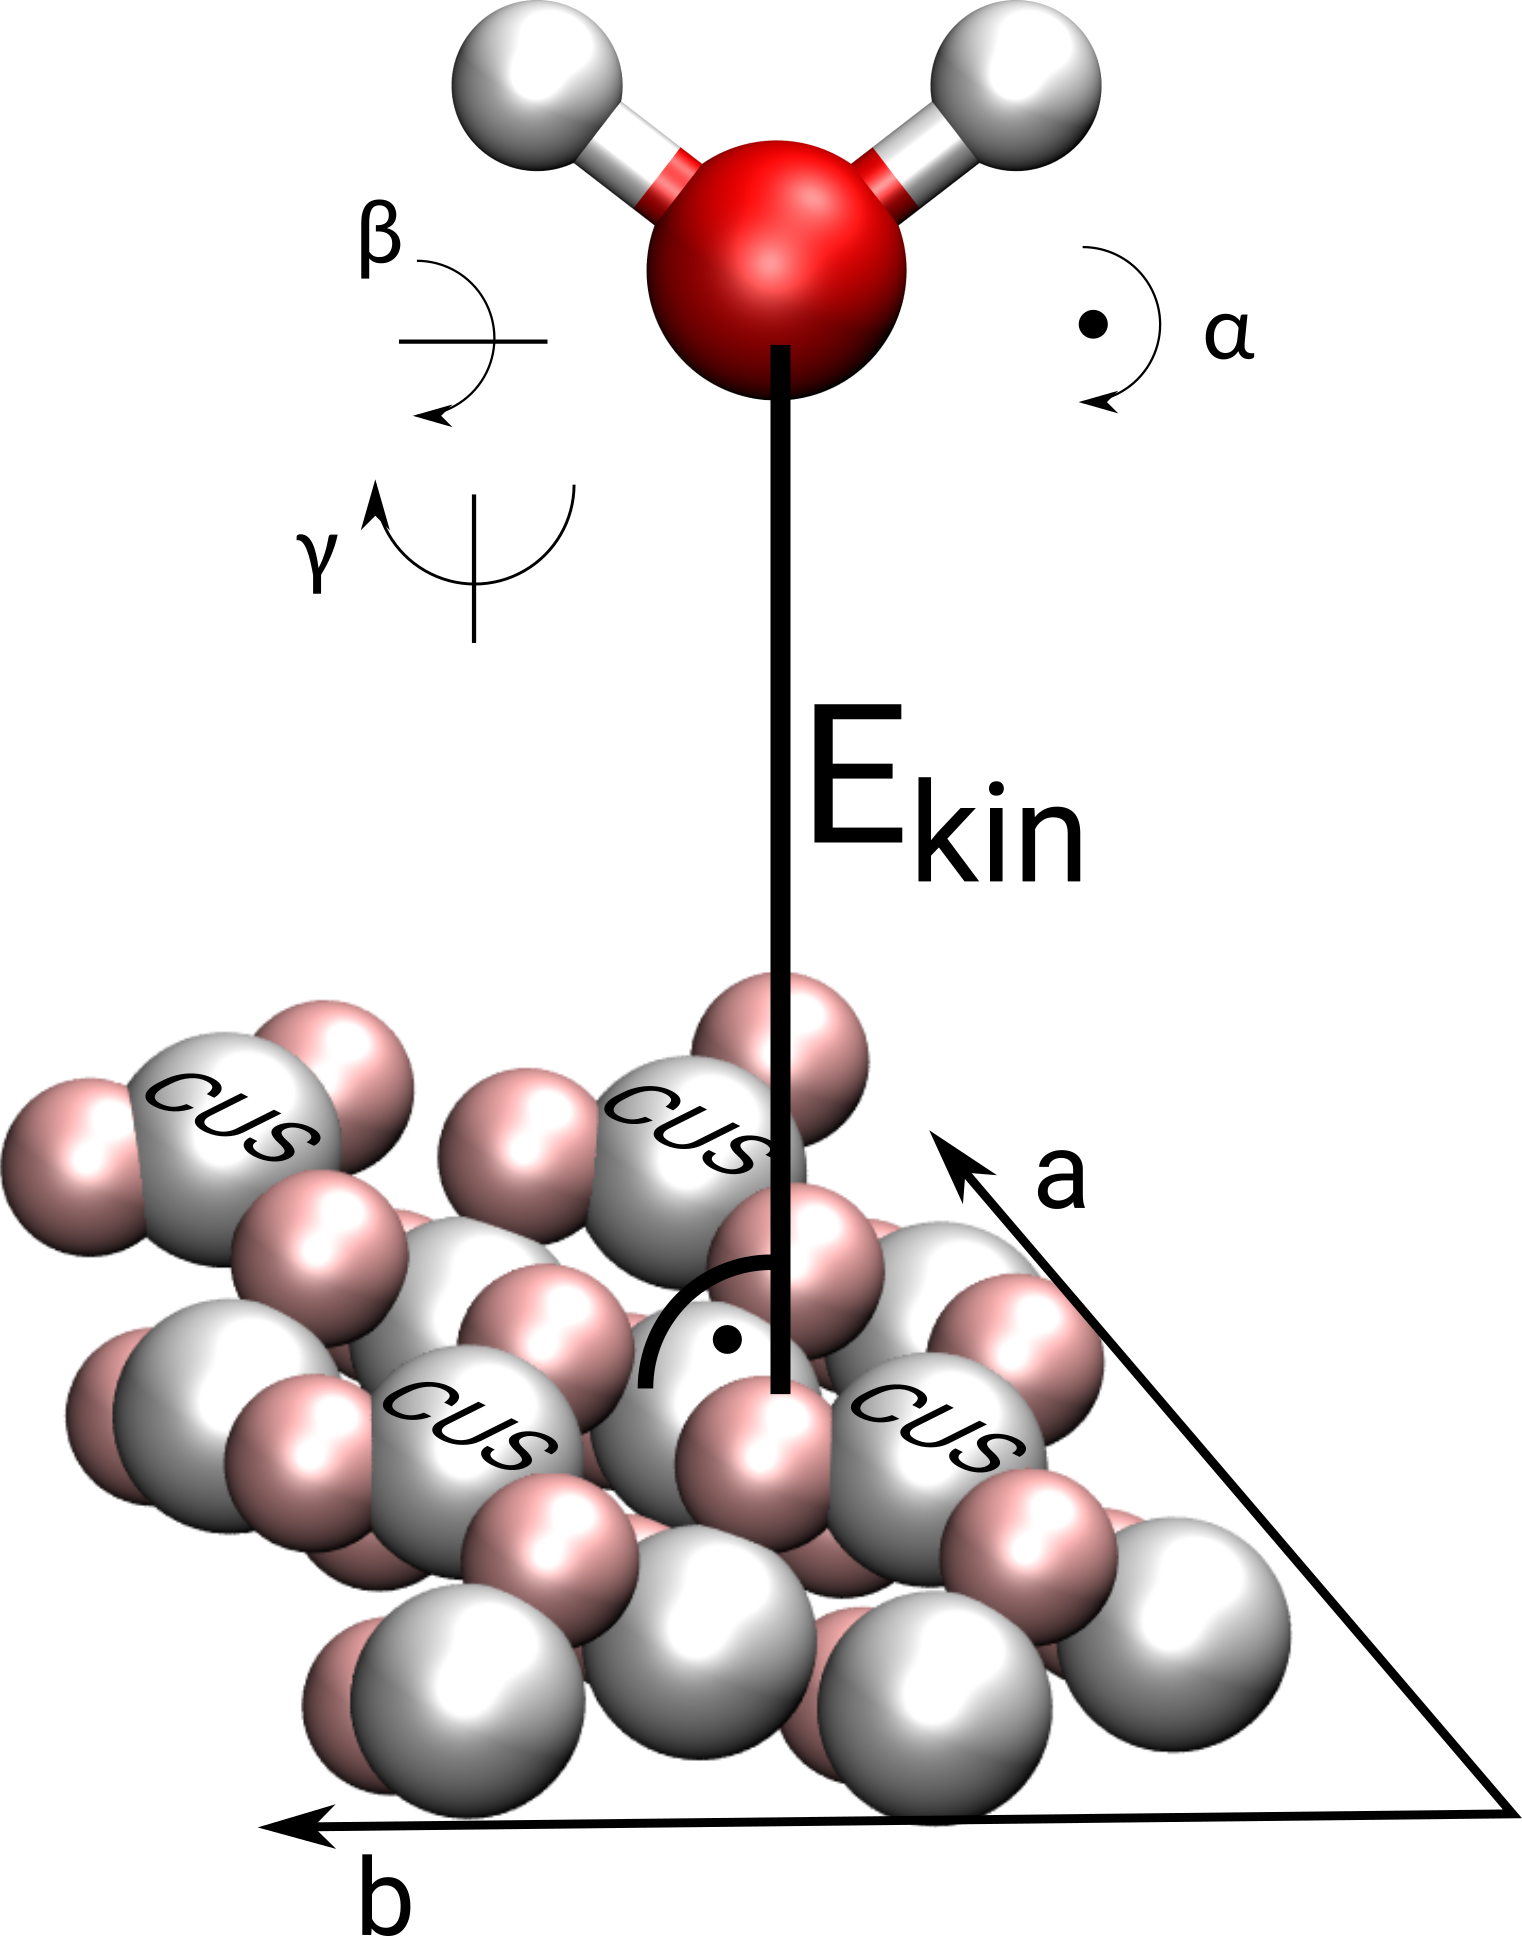
\includegraphics[width=0.3\textwidth]{figures/0001/perspective+h2o_new.png}
 \caption{Sketch for inital parameters of the trajectories. The water molecule is situated $4\,$\AA{} above the surface and is arranged within the shown coordinate system, before being shot onto the surface with a defined kinetic energy E$_\textrm{kin}$.}
        \label{abb:initial_parameters}
 \end{figure}
 
 \begin{figure}[h!]
 \centering
 \subfigure[{[0.33,0.33]}]{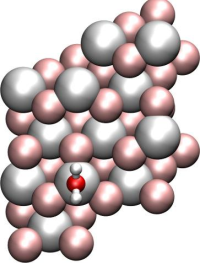
\includegraphics[angle=90, scale=0.45]{figures/0001/0_33-0_33test.png}}
          \quad
 \subfigure[{[0.5,0.5]}]{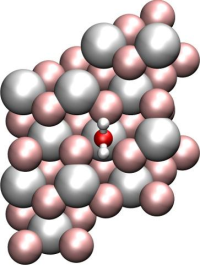
\includegraphics[angle=90,scale=0.45]{figures/0001/0_5-0_5test.png}}
         \quad
 \subfigure[{[0.35,0.5]}]{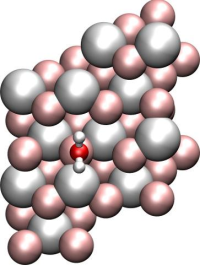
\includegraphics[angle=90,scale=0.45]{figures/0001/0_35-0_5test.png}}
        \\
 \subfigure[{[0.5,0.35]}]{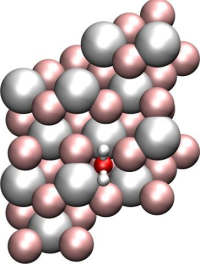
\includegraphics[angle=90,scale=0.45]{figures/0001/0_5-0_35test.png}}
        \quad
 \subfigure[{[0.35,0.45]}]{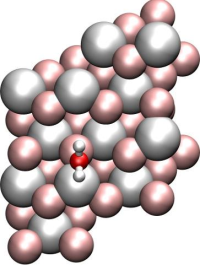
\includegraphics[angle=90,scale=0.45]{figures/0001/0_35-0_45test.png}}
        \quad
 \subfigure[{[0.4,0.5]}]{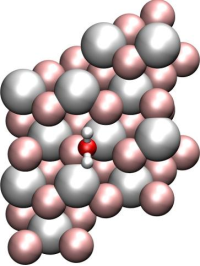
\includegraphics[angle=90,scale=0.45]{figures/0001/0_4-0_5test.png}}
 \caption{The six impact points $[a_0,b_0]$ that were used in the AIMD calculations (shown for the rotational orientation $[0,0,0]$, topview).The different points reflect the most important sites of the surface, [0.33,0.33] is on top of an Al CUS, [0.5,0.5] on top of an Al in a lower layer. [0.35,0.5] is on top of a surface oxygen atom, whereas [0.5,0.35] is on top of a subsurface oxygen atom. [0.35,0.45] is in a gap between an Al CUS and a surface oxygen and [0.4,0.5] is in the gap between a surface O and a subsurface Al atom.}
        \label{abb:impact_points}
 \end{figure}
 
 \begin{table}[!h]
 \centering
  \caption{Orientations of the water molecule. Shown are both top view and side view at impact point 0.5,0.5. (look from the right-hand side to the top view)}
 \begin{tabular}{cp{4cm}p{4cm}}
 orientation ($\alpha,~\beta,~\gamma$)& top view & side view \\\hline
 (0, 0, 0)  & 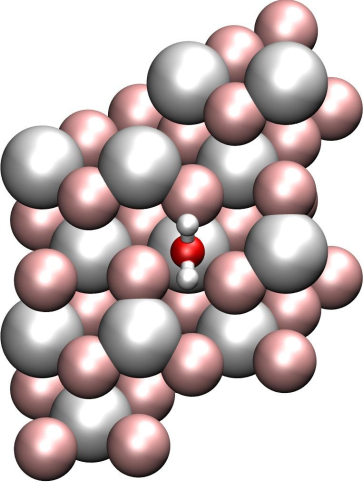
\includegraphics[width=2cm,angle=90]{figures/0001/Ausrichtungsbilder/0_0_0-toptest.png}
&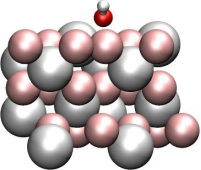
\includegraphics[width=2.5cm]{figures/0001/Ausrichtungsbilder/0_0_0-sidetest.png}\\
(0, 0, 90)   & 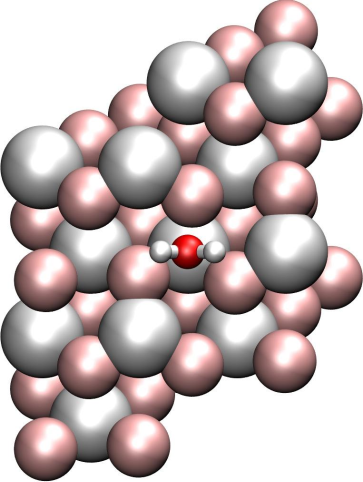
\includegraphics[width=2cm,angle=90]{figures/0001/Ausrichtungsbilder/0_0_90-toptest.png}
& 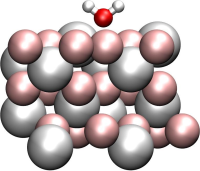
\includegraphics[width=2.5cm]{figures/0001/Ausrichtungsbilder/0_0_90-sidetest.png}\\
(0, 90, 0)   & 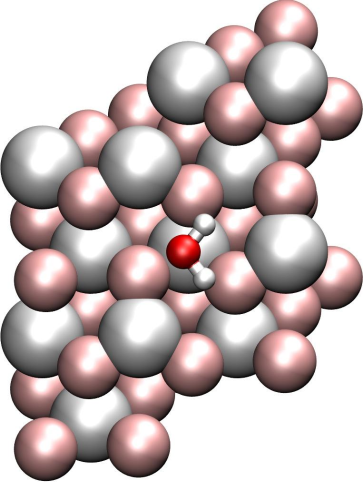
\includegraphics[width=2cm,angle=90]{figures/0001/Ausrichtungsbilder/0_90_0-toptest.png}
& \includegraphics[width=2.5cm]{figures/0001/Ausrichtungsbilder/0_90_0-sidetest.png}\\
(0, 90, 90) & \includegraphics[width=2cm,angle=90]{figures/0001/Ausrichtungsbilder/0_90_90-toptest.png} 
& \includegraphics[width=2.5cm]{figures/0001/Ausrichtungsbilder/0_90_90-sidetest.png}\\
(90, 0, 0) &\includegraphics[width=2cm,angle=90]{figures/0001/Ausrichtungsbilder/90_0_0-toptest.png} 
& \includegraphics[width=2.5cm]{figures/0001/Ausrichtungsbilder/90_0_0-sidetest.png}\\
(90, 0, 90) & \includegraphics[width=2cm,angle=90]{figures/0001/Ausrichtungsbilder/90_0_90-toptest.png} 
& \includegraphics[width=2.5cm]{figures/0001/Ausrichtungsbilder/90_0_90-sidetest.png}\\
(90, 90, 0) &\includegraphics[width=2cm,angle=90]{figures/0001/Ausrichtungsbilder/90_90_0-toptest.png} 
& \includegraphics[width=2.5cm]{figures/0001/Ausrichtungsbilder/90_90_0-sidetest.png}\\
(90, 90, 90) & \includegraphics[width=2cm,angle=90]{figures/0001/Ausrichtungsbilder/90_90_90-toptest.png} 
& \includegraphics[width=2.5cm]{figures/0001/Ausrichtungsbilder/90_90_90-sidetest.png}\\
\end{tabular}
 \label{tab:orientations}
\end{table}
 
\subsection{Example Trajectories}
Before going to the details, example trajectories for each process leading to one of the four most stable adsorbed species, molecular adsorption, 1-2 dissociation, 1-4 dissociation and 1-4$^\prime$ dissociation are shown in Figure~\ref{abb:ex_traj}, the applied parameters are reported in the respective caption. These figures were all obtained from canonical calculations (NVT) at $300\,$K (see Figure~\ref{abb:ex_traj}, the trajectory shown in (d) was additionally preexcited in the asymmetric stretch mode leading to 1-4$^\prime$ dissociation). As one can see, molecular, 1-2 and 1-4 dissociated species can occur directly at the impact time of the water molecule at the surface and is henceforth called direct dissociation from the gas phase. For the 1-4$^\prime$ dissociation shown in Figure \ref{abb:ex_traj}(d), this process does not happen directly at the impact but (in this case) ca. $40\,$fs later, so this is referred to as indirect dissociation with a molecular intermediate. This indirect process is not unique for the 1-4$^\prime$ dissociated species, all the other species including the molecular can be observed to happen indirectly by either being reflected first from the surface before adsorbing/dissociating or by adsorbing molecularly before dissociating. However, the 1-4$^\prime$ species was the only one that could not be observed after direct dissociation.

  \begin{figure}[h!]
\begin{center}
\hspace*{-1cm}
\begin{tabular}{cc}
\hspace*{-1cm}
(a) molecular adsorption & (b) 1-2 dissociation \\
{\includegraphics[width=0.4\textwidth]{figures/0001/graphs/mol.eps}}
         &
{\includegraphics[width=0.4\textwidth]{figures/0001/graphs/1-2.eps}} \\
 (c) 1-4 dissociation & (d) 1-4' dissociation \\
{\includegraphics[width=0.4\textwidth]{figures/0001/graphs/1-4.eps}} &
{\includegraphics[width=0.4\textwidth]{figures/0001/graphs/1-4d.eps}}
\end{tabular}
\end{center}
\caption{{\color{blue} Examplary trajectories for trajectories of different initial parameters, leading to the four adsorption states of water at the $\upalpha$-Al$_2$O$_3$(0001) surface as indicated in Figs.\ref{abb:0001_ads}(a)-(d). For all cases these are canonical (NVT) trajectories at  $T=300$ K. The initial parameters: (a) $E_\textrm{kin}=0.7$ eV, $[a_0,b_0]=[0.33,0.33]$, $[\alpha,\beta,\gamma]=[0,0,90]$ (in \textdegree);
 (b) $E_\textrm{kin}=0.7$ eV, $[a_0,b_0]=[0.35,0.45]$, $[\alpha,\beta,\gamma]=[0,0,0]$;
 (c) $E_\textrm{kin}=0.7$ eV, $[a_0,b_0]=[0.33,0.33]$, $[\alpha,\beta,\gamma]=[0,90,0]$;
 (d) $E_\textrm{kin}=0.7$ eV, $[a_0,b_0]=[0.35,0.5]$, $[\alpha,\beta,\gamma]=[0,0,0]$, and the water molecule 
 was vibrationally preexcited along the asymmetric stretch normal coordinate as specified in Subsec. \ref{preex}. The $r$ values indicate bond lengths between water-O and the CUS Al atom on which either D$_2$O or the water hydroxyl unit OD adsorb (O-Al), the distance between water-O and D in non-dissociated (fragments of) D$_2$O (O-D or O-D$_\textrm{ads}$), and the  distance between water-O and D in dissociated (fragments) of D$_2$O (O-D$_\textrm{diss}$), respectively. The corresponding interatomic distances of the adsorbed species from the static DFT calculations reported in Figs.\ref{abb:0001_ads}(a)-(d) are shown as horizontal, dashed lines. In (d), the 1-4$^\prime$ state is reached \textit{via} a 1-2 dissociation intermediate, which is very short-lived around $0.1\,$ps.}}
\label{abb:ex_traj}
\end{figure}

\subsection{Microcanonical AIMD at clean surface}\label{sec:mic_clean}
{\color{red} All those tables in the appendix?}\\
The effects of a single D$_2$O shot to the cool surface with a NVT ensemble (microcanonical AIMD) were studied systematically by probing over 5 different kinetic energies (from $0.5$ to $0.9\,$eV in $0.1\,$eV steps), six lateral impact points at the surface ([0.33,0.33], [0.5,0.5], [0.35,0.5], [0.5,0.35], [0.35,0.45], [0.4,0.5], see also Figure~\ref{abb:impact_points}) and eight different orientations of the water with respect to the surface ([0,0,0], [0,0,90], [0,90,0], [0,90,90], [90,0,0], [90,0,90], [90,90,0], [90,90,90], see also Tab.\ref{tab:orientations}). These $5\times 6\times 8=240$ AIMD trajectories for the clean surface at $T=0\,$K were carried out for ca $1.2\,$ps each.
\\
In the trajectories  either molecular adsorption, 1-2 dissociation or reflection could be observed. Dissociation was assumed, if the OD distance was greater than $1.3\,$\AA{}, but it was made sure that the results did not differ for a greater cutoff distance. Interestingly, only 1-2 dissociation and no 1-4 dissociation could be observed for the conditions (NVT, clean surface), although the molecular and the 1-4 dissociated species are almost equal in energy, and also the barrier heigths for the dissociation to 1-2 ($0.13\,$eV) and 1-4 ($0.19\,$eV) do not differ largely. As it is shown later, other conditions are necessary for reaching 1-4 dissociation.
\\
  \begin{figure}[h!]
\centering
 \subfigure[Energy]{\includegraphics[width=0.3\textwidth]{figures/0001/graphs/E.png}} 
 \quad
 \subfigure[Impact Point]{\includegraphics[width=0.3\textwidth]{figures/0001/graphs/impactpoint.png}} 
 \quad
 \subfigure[Orientation]{\includegraphics[width=0.3\textwidth]{figures/0001/graphs/orientation.png}}
\caption{{\color{blue} Statistics of AIMD trajectories at $T=0$ (NVE), for single D$_2$O approaching a clean alumina(0001) surface. In (a), for each of the five different initial kinetic energies $E_\textrm{kin}$, results are averaged over the $6 \times 8=48$ combinations of impact sites and rotational orientations. In (b), for each of six different initial impact points $[a_0,b_0]$, results are averaged over $5 \times 8=40$ combinations of kinetic energies and rotational orientations. In (c), each of the eight different initial rotational orientations $[\alpha,\beta,\gamma]$, results are averaged over $5 \times 6=30$ combinations of kinetic energies and impact points. Columns show percentages of trajectories leading to  reflection (``refl''), molecular adsorption (``mol''), and  direct and total 1-2 dissociation (``1-2 diss direct'' and  ``1-2 diss total''). (No columns if no trajectories of the  type were found.)}}
\label{abb:barchart_mic}
\end{figure}
For a statistical analysis of the data see Figure~\ref{abb:barchart_mic}, where the probabilities for reflection, molecular adsorption and 1-2 dissociation are shown as a function of the kinetic energy (a), impact point (b) and the orientation (c). There also between direct and indirect dissociation is distinguished. Admittedly, this analysis is restricted by the number of trajectories (240). From these figures and the data one can derive the following conclusions:
\\
As anticipated, all three processes could be observed, reflection ($20.4\%$, 49 of the 240 trajectories), molecular adsorption ($55.4\%$, 133 trajectories) and 1-2 dissociation ($24.2\%$, 58 trajectories).
\\
Looking at the impact of the energy in Figure \ref{abb:barchart_mic}(a), the result do not depend largely on the initial kinetic energy of the molecule, at least for the probed energy range. In all cases molecular adsorption dominates, followed by 1-2 dissociation and reflection, that are in the same range around $20$-$25\%$. This reflecion probability P$_\textrm{diss}$ is only increased for $0.9\,$eV, at the expense of the molecular species. To tackle the low energy regime, one additional trajectory of $0.1\,$eV was done ([$a_0,b_0]=[0.35,0.45]$; $[\alpha,\beta,\gamma]=[0,0,0]$), for which $P_\textrm{diss}=1$ for all energies $\geq 0.5\,$eV. In the case of E$_\textrm{kin}=0.1\,$eV, the trajectory only shows molecular adsorption. This result was rather surprising, since the kinetic energy plus the adsorption energy minus the barrier height is with ($0.1+1.31-0.13$)eV=$.28\,$eV larger than the reaction barrier. It seems that the excess energy is not available for the OD-bond breaking and instead relaxes in other degrees of freedom of the system. That allows to draw the conclusion, that a minimum kinetic energy is necessary for the dissociation process. In the experiments of R. K. Campen, a kinetic energy of the beam between $0.6$ and $0.75\,$eV is used. This minimum energy constraint can be one possible explanation of the difference between MBS and pinhole dosing. In the latter case, the only energy of a water molecule comes from the thermal energy that is for a D$_2$O molecule in the gas phase at $300\,$K around $\frac{3}{2}k_BT\approx40\,$meV.
\\
In contrast to the kinetic energy, the lateral impact point at the surface has a great influence on adsorption and dissociation probabilities (see Figure \ref{abb:barchart_mic}). For the impact point [0.5,0.5], that is at a  non-surface Al position, $88\%$ of the trajectories get reflected and molecular adsorption and 1-2 dissociation are oppressed, whereas for [$0.33,0.33$], directly on top of an Al CUS position, $83\%$ adsorb molecularly which dominates clearly over 1-2 dissociation. In contrast to both sites, [$0.35,0.45$] which is a gap between a CUS position and a neighboring oxygen atom leads to a high dissociation probability of P$_\textrm{diss}\approx 68\%$ with a minor percentage of indirect dissociation. This high dissociation probability can be explained by the fact, that the molecule hits the surface already in a ``product-like'' geometry, so that the OD bond breakage is facilitated.
\\
The initial rotational orientation has also an effect, although not so clearly as for the impact point. This might be explained when looking at the trajectories in detail, so one can see, that the water molecule rotates due to the attractive and repulsive interaction with the surface atoms, that lead to a reorientation of the water molecule right before adsorbing, so that the initial orientation is not remembered by the system. The orientation that the molecule is in shortly before reaching the surface is more important, also here, if the molecule's orientation is already in a product-like state, the dissociation probability is elevated.
\\
As can be seen from the data, direct dissociation dominates mostly over indirect dissociation, although it is dependend from the initial conditions, e.g. for the initial orientation [0,90,90] only indirect dissociation is observed (cf. Figure \ref{abb:barchart_mic}(c)).

 
\subsection{Thermalized Surface}\label{therm_surf}
After getting an impression about the system with the microcanonical MD with the clean surface, as a next step the thermalized surface at $300\,$K is studied. For this the naked surface was preequilibrated at $300\,$K for $1\,$ps and the obtained geometry with the included velocities was used as an input to the following calculations. Here, only a kinetic energy of $0.7\,$eV was considered, since this energy is the closest to previous experiments by Kramer and also the energy dependence was shown to be very low. The water molecule was then shot onto the equilibrated surface and the heat bath acted from the start on the water molecule. This is not a problem, since the molecule hits the surface quickly and thus hardly affects the dynamics.
\\
First, for a selection of 5 parameter sets 100  NVT trajectories were calculated each at a temperature of $300\,$K. These parameter sets are $[a_0,b_0][\alpha,\beta,\gamma]$= $[0.35,0.45]$,$[0,0,0]$; $[0.35,0.45]$,$[0,90,90]$; $[0.35,0,45]$,$[90,90,90]$; $[0.4,0.5]$,$[0,0,0]$;  $[0.5,0.35]$,$[90,0,90]$. These parameters led in the previous microcanonical ensemble to 1-2 dissociation and were chosen because the idea was that the thermal effects might trigger them to dissociate or diffuse to the 1-4 species. The duration of the trajectories was $1\,$ps and were done analogously to \ref{sec:mic_clean} except for now the thermalized surface. All of these 500 trajectories dissociated 1-2, no reflection, molecular adsorption or further dissociation could be observed. As it seems, the thermal contribution is low, which was unexpected. The energy of the thermalized surface can be estimated by $N_s\times 3k_BT=2.8\,$eV (with $N_s=36$ being the number of atoms in the surface slab that were allowed to relax/move). This energy is in the same range as the kinetic energy of the incoming water molecule ($\approx2\,$eV). Indeed, this surface energy is not valid for the small surface range where the impact takes place, so that the thermal energy of the atom(s) of the impingement is considerably smaller.
\\
As a next step, for all $6\times 8=48$ combinations of parameters, but with the thermalized surface, were done for all 6 impact points and 8 orientations presented in Section \ref{sec:mic_clean}, but only for a kinetic energy of $0.7\,$eV. For each of the sets, two trajectories of $4\,$ps duration were calculated. This restriction is due to high computational costs and  gives rise to only a limited statistical significance. The long duration accounts for processes that occur later after the impact, that could have been missed by shorter trajectories. In Table \ref{tab:nvt-nve_comp}, the probabilities for each process is shown, in comparison with the previous microcanonical AIMD trajectories. Because 6 of the trajectories aborted due to numerical reasons, here only 42 trajectories can be evaluated and the comparison is, of course, done only with the corresponding microcanonical trajectories.
\begin{table}[!h]
 \centering
 \caption{{\color{blue} Statistics for NVE (upper two lines) and NVT ($T=$ 300 K, lowest line) AIMD trajectories. The initial impact parameters $[a_0,b_0]$ and $[\alpha,\beta,\gamma]$ were (selected from) the 48 impact parameters used in Sec. \ref{sec:mic_clean} as desribed in the text. In all cases, a single water molecule with initial $E_\textrm{kin}=0.7$ eV was fired on a clean surface.}}
\vspace*{.2cm}
  \begin{tabular}{lc|cccc}
 \hline
  ensemble & no. of trajectories & $P_\textrm{refl}$ & $P_\textrm{mol}$ & $P_\textrm{diss}$ (1-2) & $P_\textrm{diss}$(1-4) 
 \\\hline
 NVE$^1$         & 48 & 0.19 & 0.58 & 0.23 & 0.00 \\
 NVE$^{1,3}$     & 42 & 0.19 & 0.55 & 0.26 & 0.00 \\
 NVT$^2$ &$42\times 2$& 0.12 & 0.54 & 0.24 & 0.11 \\\hline
  \end{tabular}
\begin{tablenotes}
 \footnotesize
\item[] $^1$ Propagation time $1.22$ ps. $^2$ Propagation time 4 ps. $^3$ A subset of the NVE/48 data set,  corresponding to the same initial impact parameters as used for the NVT ensembles.
\end{tablenotes}
\label{tab:nvt-nve_comp}
\end{table}
In the first line of the table, the results for the complete probed space for the NVE (T=0) is shown, the second line gives the results for the corresponding 42 microcanonical trajectories and in the third line, the canonical results for 42 NVT trajectories ($T=300\,$K) are given. For all, the kinetic energy is $E_\textrm{kin}=0.7\,$eV. In contrast to the microcanonical MD, the canonical show 1-4 dissociation at a percentage of around $11\%$ and slight decreases in the reflection, whereas molecular adsorption and 1-2 dissociation almost are equal. From the 1-4 dissociated trajectories, $44\%$ dissociated directly and $56\%$ indirectly after initial molecular adsorption. Interestingly, all inital conditions in the trajectories that show 1-4 dissociation in the NVT led only to molecular adsorption in the NVE AIMD.
\\
Note, that the surface temperature indeed has an effect on the probabilities for the different processes and also 1-4 dissociation could be observed.
As before, the first impact can lead to reflection and in a ``bouncing'' process, the molecule can also adsorb after another impact, in some cases also on another CUS atom as the initial impact was on.
 
\subsection{Refined Surface Model}
In the experiment, after a certain time, the coverage will be higher, which will have an impact on the incoming molecule. To account for this a preadsorbed surface model was applied, where the minimum structure of the surface with a single adsorbed water molecule was used and a second D$_2$O was sent onto this surface. For the preadsorbed water, the three minima were assumed: (a) the molecular minimum, (b) the 1-2 dissociated species and (c) the less stable 1-4 dissociated water. The preadsorbed OD/D$_2$O was adsorbed at the position [0.33,0.33], in the lower right $1\times 1$ sub cell of the super cell in Figure \ref{abb:0001_ads}, that is located around the CUS atom at this lateral impact point.
\\
For the incoming second water molecule with an initial kinetic energy of $0.7\,$eV, one has to distinguish two cases: The impact points [$a_0,b_0$] were chosen such that (i) the second water molecule is shot in the same $1\times 1$ sub cell where the preadsorbed water is adsorbed (the lower right part of the super cell) and (ii) in another sub cell, here, the lower left part. Once again, various initial orientations and impact points were probed for a propagation time of $1\,$ps.
\\
First, NVE (microcanonical, $T=0\,$K of the initial surface) were done. (i) In the first case, the incoming water is shot to the vecinity (same sub cell) of the preadsorbed molecular water, the second \textit{incoming} D$_2$O is observed to be either reflected or adsorb molecularly at another CUS atom after initial reflection from the preadsorbed water molecule. In the case of molecular preadsorbed water, the impact of the second molecule can make the molecular \textit{preadsorbed} water dissociate to 1-2, 1-4 and even 1-4$^\prime$. Assumingly, part of the energy is not used to overcome the barrier to diffusion/dissociation but to interaction with the preadsorbed molecular species. The same does not happen for the 1-2 and the 1-4 preadsorbed species only in one case reacts to the molecular adsorbed species. As can be seen in Table \ref{tab:preads_mic}, there is a difference between impact points direct on the CUS atom ($[0.33,0.33]$) and the impact position next to the CUS position $[0.35,0.45]$. Additional data is shown in the Appendix.
\begin{table}[!h]
  \centering
  \caption{{\color{blue} Outcome of selected microcanonical (NVE, $T=0$) trajectories with $E_{\textrm{kin}}=0.7\,$eV, after the end of propagation, for three cases of a single water molecule being molecularly or dissociatively preadsorbed on the surface. R=reflection, M= molecular adsorption (chemisorption), P=molecular physisorption, D(1-2)=1-2 dissociation, D(1-4)=1-4 dissociation. In each entry, the first letter gives the outcome for the \textit{incoming} molecule, the second one the fate of the preadsorbed species. In case the latter has changed its character, a $*$ was added. ``term.'' means terminated trajectory. Where no entry was made, no calculation was performed.}}
\hspace*{-1cm}
 \begin{tabular}{l|cc|cc|cc}
 \toprule
               & \multicolumn{6}{c}{type of preadsorption } \\\hline
               & \multicolumn{2}{c|}{molecular} & \multicolumn{2}{c|}{1-2 dissociated} & \multicolumn{2}{c}{1-4 dissociated} \\\hline
    orientation& \multicolumn{2}{c|}{impact position $[a_0,b_0]$} & \multicolumn{2}{c|}{impact position $[a_0,b_0]$} & \multicolumn{2}{c}{impact position $[a_0,b_0]$} \\
    $[\alpha,\beta,\gamma]$ & [0.33,0.33] & [0.35,0.45] & [0.33,0.33] & [0.35,0.45] & [0.33,0.33] & [0.35,0.45] \\
    \midrule
   $[0,0,0]$    &          & P, D(1-2)$^*$  &  & M, D(1-2) &  & R, D(1-4) \\
   $[0,0,90]$   &          & M, D(1-2)$^*$  &  & M, D(1-2) &  & P, D(1-4) \\
   $[0,90,0]$   & M, D(1-2)$^*$ & P, D(1-4)$^*$  & R, D(1-2) & M, D(1-2) & R, D(1-4) & P, D(1-4) \\
   $[0,90,90]$  &          & P, D(1-4')$^*$ &  & M, D(1-2) &          & term. \\
   $[90,0,0]$   &          & P, D(1-2)$^*$  &  & M, D(1-2) &  & M, D(1-4) \\
   $[90,0,90]$  &          & P, M      &  & D(1-2), D(1-2) &  & P, D(1-4) \\
   $[90,90,0]$  &          & P, D(1-4)$^*$  &  & M, D(1-2) &  & R, D(1-4) \\
   $[90,90,90]$ & M, D(1-2)$^*$ & P, D(1-4)$^*$  & R, D(1-2) & M, D(1-2) & M, D(1-4) & P, D(1-4)
\\\hline
  \end{tabular}
  \label{tab:preads_mic}
\end{table}

Considering the impact point [0.33,0.33] of the incoming water, that is exactly where the preadsorbed water is located, one can see either reflection (R) or molecular adsorption after diffusion to another CUS site (M in Table \ref{tab:preads_mic}).\\
In contrast to that, an impact point near the CUS atom, [0.35,0.45], gives rise to a greater number of different outcomes. In the case of the molecular preadsorbed species, molecular adsorption on a neighboring CUS and physisorption above the preadsorbed molecular species (\textit{i.e.} the molecule is not bound directly to a CUS atom but  to water (fragments) via hydrogen bonds) can be observed, which leads to the conclusion, that clustering occurs at the surface.
For the 1-2 dissociated preadsorbed system, also 1-2 dissociation on a neighboring CUS can be discovered. The 1-4 dissociated preadsorbed species gives in addition to molecular adsorption, physisorption also reflection.
If the preadsorbed species is dissociated, molecular adsorption is clearly favored, followed by physisorption.
\\
Looking at the preadsorbed species, the molecular species is mostly affected by the incoming molecule by showing dissociation to all dissociated states (1-2, 1-4 and also 1-4$^\prime$), whereas the 1-2 dissociated preadsorbed species is not influenced at all. Only for one of the 1-4 preadsorbed trajectories, a change of the state is observed, to a molecular species via proton transfer from the incoming water molecule.
\\
(ii) In the second case, a neighboring sub cell (the lower left one) is the aim of the molecular beam, where no water is preadsorbed. The preadsorbed water or water fragments are hardly disturbed by the incoming D$_2$O, due to the great distance of the residues. Only a single trajectory out of 36 changed its character, namely the molecularly preadsorbed species exchanged a proton with the neighboring 1-2 dissociated incoming species after the impact and therefore dissociated.
\\
Surprisingly, the incoming molecule is affected by the preadsorbed species in the way that  the dissociation probability is increased and 1-4 dissociation occurs, in contrast to comparable previous microcanonical with a clean surface: Mostly molecular adsorption (P$_\textrm{mol}$=0.47), dissociation (P$_\textrm{1-2}$=0.22 and P$_\textrm{1-4}$=0.14), physisorption (P$_\textrm{phys}$=0.11) take place. Reflection is drastically decreased (P$_\textrm{refl}$=0.06). [Respective values for microcanonical MD of the clean surface are P$_\textrm{mol}$=0.58, P$_\textrm{1-2}$=0.23, P$_\textrm{1-4}$=0, P$_\textrm{phys}$=0 and P$_\textrm{refl}$=0.19]. Although the statistics may not be sufficient, the reduced probability of reflection can be interpreted with attractive interaction of both the incoming and the preadsorbed molecule and leads to a higher probability of dissociation.
\\
Summarizing these findings, one can say, that the preadsorbed enhancement of the system leads to further outcomes of the scattering as physisorption/clustering on the surface and the so far unreached 1-4 and 1-4$^\prime$ species, the latter by dissociation of preadsorbed molecular water.
As it is not surprising, the influence is bigger with the incoming water molecule being near the preadsorbed species.
\\
In analogy to these NVE trajectories, canonical (NVT with $T=300\,$K) trajectories with the preadsorbed systems were done. As before (Section \ref{therm_surf}), as a starting point the preequilibrated structures of molecular adsorption, 1-2 and 1-4 dissociation were used, that were equilibrated at $300\,$K for $1\,$ps. The following trajectories including the $0.7\,$eV water ``beam'' were run for $1\,$ps. As for the respective microcanonical trajectories, one has to distinguish between the water aiming at (i) the same sub cell (lower right) and (ii) the neighboring sub cell (lower left 1$\times$ 1 sub cell). The results do not differ largely, but some probabilities are altered.
For case (i) in comparison with the microcanonical preadsorbed surface one can see that only physisorption is enhanced, whereas the other processes (molecular adsorption, 1-2, 1-4 dissociation and reflection) are suppressed. In the case of the water hitting the neighboring subcell (ii) similar effects can be seen, although here molecular adsorption is favored and the other processes (1-4 dissociation, physisorption and reflection) are reduced, and 1-2 dissociation happens with almost the same amount as in the NVE ensemble. Also concerning the preadsorbed water (fragment) there are changes, especially for the molecular preadsorbed species in case (i): Only in 4 out of 24 cases the character of the preadsorbed water changes.
For the case of molecular preadsorption and the neighboring CUS, there is an increase in the molecular adsorption (P$_\textrm{1-2}$=0.34 instead of 0.23 for microcanonical) leads to the conclusion, that the influence of the preadsorbed species is high despite the distance so that the non-locality of the process is enhanced.

\subsection{Refined Beam Model}
Enhancing the beam is a further refinement and is done here in two different ways: assuming a water cluster as the approaching species and as a second improving method exciting the water molecule rotationally, vibrationally and with a combination of both.
\subsubsection{Clustering}\label{clusters}
As a cluster, the (D$_2$O)$_4$ system was optimized in the same periodic boundary conditions as the cell before but without the surface, for geometry see Figure \ref{abb:D2Ocluster}. The same cluster was already shown to be the most stable one by Wales et al.\cite{Wales97}, there it is called ``up-down-up-down''. This cluster was then fired with a kinetic energy of $0.9\,$eV at the cold clean surface (NVE) from a distance of $4\,$\AA{} above the Al surface layer, with a duration of around $1.22\,$ps. Once again, several impact points and orientations of the cluster were considered. These orientations were applied analogously to the previous ones with the axes of the rotations shown in Figure \ref{abb:D2Ocluster}(b).
\\
\begin{figure*} [!ht]
\centering
 \subfigure[Geometry]{\includegraphics[width=.55\textwidth]{figures/0001/4H2O.pdf}}
  \quad
\subfigure[Coordinate system]{\includegraphics[width=.35\textwidth]{figures/0001/4d2o_axes.png}}
\caption{(D$_2$O)$_4$ cluster for simulation of effects of higher coverages. (a) shows the geometry, especially the DOD bond angle and the OD bond length of neighboring molecules and (b) shows the coordinate system for the rotations along the axes.}
       \label{abb:D2Ocluster}
\end{figure*}
Evaluating the data shows that the cluster breaks up upon contact with the surface into individual D$_2$O molecules and these undergo different processes, to a great extent influenced by the surrounding water molecules, due to the high coverage of $1\,$ML. The water can adsorb molecularly or dissociatively (both directly and indirectly), physisorb, Deuterium atoms can diffuse or single molecules can be reflected totally.\\
{\color{blue} example trajectories/final figure for cluster calculations?}\\
Mostly independent of the settings, the molecules interact strongly with each other showing a profoundly dynamic behavior. This gives rise to processes that were not possible for the clean surface NVE and a single water situation, where no 1-4 dissociation nor physisorption was observed. Of course, the probabilities for dissociation, molecular adsorption and reflection are different, the probability of molecular adsorption is strongly diminished to the advance of 1-2, 1-4 and 1-4$^\prime$ dissociation and physisorption. For details see Appendix.
\\
{\color{red} \textit{Mention here, in the appendix or not at all?!} Also one type of (D$_2$O)$_2$ was tested (see Figure \ref{abb:D2O2clusters}). The structure is not the minimum structure but another dimolecular water cluster. Even in the case of the (D$_2$O)$_2$ cluster, strong interaction between the molecules can be observed, although not as much as for the tetramer. Also ``only'' molecular adsorption, 1-2 and 1-4 dissociation occur within the sampling. Interestingly, there is no case, where both molecules react in the same way. For most dissociated trajectories there is only direct dissociation at the moment of the impact, with the only one dissiciating $0.3\,$ps later. Apart from that, no further dissociation and diffusion reactions were observed.
}
\begin{figure}[!t]
\centering
\subfigure[(D$_2$O)$_2$]{\includegraphics[width=0.33\textwidth]{figures/0001/2H2O.pdf}}
         \quad
\subfigure[sketch of (D$_2$O)$_2$ cluster]{\includegraphics[angle=90,width=0.3\textwidth]{figures/0001/2H2Oexample.png}}
          \quad
          %add desired spacing between images, e. g. ~, \quad, \qquad, \hfill etc. (or a blank line to force the subfigure onto a new line
\caption{Structure of the optimized (D$_2$O)$_2$ cluster (a). (b) shows an example situation at the last step (after $1.2\,$ps) for 2 water molecules for the initial parameters [$a_0,b_0$]=[0.35,0.45], [$\alpha,\beta,\gamma$][90,0,90].}
       \label{abb:D2O2clusters}
\end{figure}

\subsubsection{Rotationally and Vibrationally Preexcited Water}\label{preex}
Here, qualitative results are given for  a D$_2$O molecule that is at the start of the trajectory not rigid as before but excited rotationally and/or vibrationally. It is shot with a kinetic energy of $0.7\,$eV at the clean surface in an NVE ensemble for a trajectory duration of $2\,$ps at the impact point [$0.35,0.5$] with the initial orientation [$0,0,0$]. With these applied conditions in the rigid case (microcanonical without rotational or vibrational excitation), the molecule dissociates to the 1-2 structure, the same for the thermal surface at $T=300\,$K.
\\
The vibrational excitations were chosen as follows: For the single water molecule in the periodic boundary conditions a normal mode analyses was done and the modes for the symmetric stretch, asymmetric stretch and the bending mode were used as an input for the MD trajectories in addition to the initial momentum towards the surface. For the rotational preexcitations along the three axes, D atoms were given initial momenta to induce a rotational motion corresponding to rotational energies of $\sim 0.2\,$eV.
\\
The results for the rotation around the $\gamma$-axis (cp. Figure \ref{abb:initial_parameters}) shows molecular adsorption whereas rotations around the other two axes give 1-2 dissociation as in the initial microcanonical trajectories without rotational excitation.
In the cases of vibrational preexcitation, the symmetric stretch leads to reflection, the asymmetric stretch gives 1-4$^\prime$ dissociation after initial 1-2 dissociation (as was already mentioned in Figure \ref{abb:ex_traj}) and with the bending mode being excited, the water dissociates to 1-2. Also, a small collection of combinations of vibrations with rotations were calculated, that lead to either molecular adsorption (rotation around $\alpha$? and bending mode), or 1-2 dissociation (rotation around $\gamma$ and asymmetric stretch; and rotation around $\beta$ ans symmetric stretch).
\\
Quantitatively, the results may depend strongly on the excitation energy, that was not of concern here, one can say, that preexcitation has an effect on the dynamics of the water adsorption and dissociation, respectively, that were not possible with the rigid water molecule.
\\
\\
Although a large number of trajectories were done with the contingent at the HLRN facility a reliable statistics could not be achieved. It was only computationally feasible to do trajectories with $1-4\,$ps duration. Also not all degrees of freedom could be probed, \textit{e.g.} the angle of the beam with respect to the surface other than 90\textdegree{} and initial orientations were only probed in 90\textdegree{} steps. Apart from that, no quantum effects were considered.
\clearpage

%%%%%%%%%%%%%%%%%%%%%%%%%%%%%%%%%%%%%%%%%%%%%%
\section{Improvement of Reaction Rates}\label{sec_rates}
For a model reaction we try to improve the reaction rate of a specific chosen reaction with different new methods. This reaction is a H-diffusion reaction on the (0001) surface studied before in our group, the Df-H-4-2 reaction, that moves a proton in the 1-4 position to the OH residue to the 1-2 dissociated state (see Figure \ref{abb:df-h-4-2}).
\begin{figure}[h]
\centering
\includegraphics[width=0.95\textwidth]{figures/0001/NEB-path/df-h-4-2.pdf}
\caption{Reaction path of the Df-H-4-2 proton diffusion reaction in the PBE-D2 level of theory, left is the educt (1-4), in the middle the minimum energy path with the transition state geometry as an inlay and on the right the product (1-2) of the reaction. \textit{Data with friendly permission by Jonas Wirth}.}
       \label{abb:df-h-4-2}
\end{figure}
The rates were before calculated with PBE+D2 and the implementation of Nudged Elastic Band in VASP. An approach were singlepoint calculations were done for the minima and the transition state was also done. For this process also a 1-D potential energy surface was calculated and then the Schr�dinger equation was solved to obtain the wave function and see the localization/delocalization of the reaction pathway.
\\
Now we want to expand these methods to the followin: We want to calculate the adsorption energies and the barrier within a atom centered orbital method with the hybrid functional B3LYP and also go beyond density functional theory and go to perturbation theory (LMP2).
%\\
%Apart from that, we study this reaction with the help of Path Integral Molecular Dynamics, where the system is represented as a couple of beads that are connected and henceforth act as a more delocalized particle which can contribute to quantum effects, proton tunneling.
%\\
%As a last approach, we want to apply other higher level methods in an embedded approach. We cut a cluster from the surface situation and embed this cluster in a field of point charges. By doing this we can calculate the cluster with a better method, let's say B3LYP, CCSD or MP2 and then apply a substractional scheme to get to corrected adsorption energies that can then be used to improve the rates with Eyring's equation for transtition states.

\subsection{MP2 and B3LYP}\label{crystal_calc}
Going beyond pure density functionals and also beyond DFT has been too costly for a long time, simply not applicable for surface adsorbat system that large and electron rich. In the crystal/cryscor code one uses atom centered bases instead of plane waves and so large scale systems can also be computed. We first optimized our parameters with HF calculations and then did calculations with PBE similar to prior plane wave based calculations.
\\
We found out, that BSSE takes a big part, but corrections are not easily applied because the ghosted calculations needed for that do not converge for all the structures with a bigger OH-H distance. Instead we have to use bigger basis sets containing diffuse functions in order to handle the BSSE. Such a self designed basis set by our cooperation partner Dr. Denis Usvyat (HU Berlin, group of Martin Sch\"utz) was used here. With this basis set we did the PBE calculations again (?) and the B3LYP as well as the MP2 calculations. First we compared the differences in adsorption energies. We furthermore compared the vibrational frequencies from B3LYP with the ones from VASP/PBE to see a methodological effect.
\\
We also reoptimized the transition state for the Df-H-4-2 reaction.


% \todo{Not sure if this will come into the diss? No real results obtained..?}
% \subsection{PIMD}
% Instead of examining reactions with a defined reaction pathway as with NEB, we apply the path integral MD to propagate the 1-4 dissociated state in the hope to watch the reaction and to extract from that a time for the reaction {\color{red} (? it is not really a rate)}. But unluckily, no reaction occurred in the given propagation time, so that one only can see the delocalization of the proton. At a given temperature of $300\,$K the proton only moves a little, far away from any reactive trajectory.
% \\
%  A huge problem was the unit cell: when all atoms or only a few atoms were allowed to move during the trajectory, the whole cell drifted away, as if the periodic boundary conditions would not apply. When fixing all the atoms except for the proton that diffuses it was fine.
%  \\
%  {\color{red} cell optimizations were tried, but didn't work as planned; fixing only the rim lead to other atom's movement, maybe one can free the OH group and the Al atom on which the H sits?}
%  \\
%  We used also PBE but without dispersion corrections and for the trajectories at $300\,$K we applied the Nos\'{e} Hoover thermostat.
%  
% \subsection{QM/QM Embedding Scheme}
% In order to recalculate adsorption energies and reaction rate constants with a higher level method we tried to apply the mechanical embedding scheme developed in the Sauer group from HU Berlin. One uses a substractive scheme to correct energies, after calculating the complete system with the low level method (here PBE), the interesting part, namely the cluster, with both the low level method and the high level method (B3LYP, MP2 or CCSD). The high-level:low-level corrected energy is then calculated by the following equation: \textit{equation}
% \\
% First of all, a reasonable cluster has to be chosen, which is difficult since the 1-4$^\prime$ needs a big cluster to be considered. We chose then the Al$_8$O$_{12}$-cluster used in unpublished work from the same group. This cluster was used for tests but when it came to embedding, the Turbomole package failed to compute the embedded system, because hexagonal cells were not yet implemented into the code.


\addchap{Summary}

We made great progress in understanding the (11\=20) surface of $\upalpha$-Al$_2$O$_3$ in contact with water in the low coverage regime. 
\\
The dissociation process of water on (0001) surface was studied.
\\
Several methods were tested to improve reaction rates.
%%%%%%%%%%%%%%%%%%%%%%%%%%%%%%%%%%%%%%%%%%%%%%%%%%%%%%%%%%%%%%%%%%%%%%%%%%%%%%%%%%%%%%%%%%%%%%%%%%%%%%%%%%%%%%%%%%%%%%%%%%%%%%%%%%%%%%%%%%%%%%%%%%%%%%%%%%%%%%%%%%%%%%%%%%%%%%%%%%%%%%%%%%%%%%%%%%%%%%%%%%%%%%%%%%%%%%%%%%%%%%%%%%%%%%%%%%%%%%%%%%%%%%%%%%%%%%%%%%%%%%%

\begingroup
\renewcommand{\cleardoublepage}{}
\clearpage
\addchap*{Acknowledgment}
\endgroup
I want to thank my doctoral father Prof. Dr. Saalfrank, for giving me the scientific opportunity to research on surface systems and all the valuable discussions and advices. Also I am deeply grateful to my supervisor Dr. Jonas Wirth who gave me support during my time starting as a Bachelor's student, during my Master's thesis and also through the beginning of my PhD, PD Dr. Tillmann Klamroth for discussions about programming and theoretical questions that arose during the work, Dr. Rados\l{}aw W\l{}odarczyk for his endless knowledge with vasp and programming in general, Giacomo Melani (soon to be Dr.) for his advice and his help, and also the discussions about our teaching duties in mathematics and the whole workgroup for all the valuable discussions and the help. Also for the great atmosphere, that was some times productive and some times also just relaxing and felt very comfortable, here especially Clemens Rietze, Robert Scholz, Gereon Floss, and Steven Lindner.
Also I want to thank my second supervisor Beate Paulus for discussion and help beyond research topics.
Great acknowlegdment to my experimental cooperation partners from FHI, Yanhua Yue, Dr. Harald Kirsch and Dr. Kramer R. Campen for the great work and publications we did together.
Thanks to Dr. Denis Usvyat for all his patience and knowledge and valuable discussions about crystal/cryscor and his help.
Maristella Alessio from Sauer group (HU Berlin) for help with Turbomole and setting the mechanical embedding calculations, that unluckily did not work for the applied cluster.
Ji Chen and Wei Fang from Michaelides group from UCL London for their help with cp2k and i-Pi, necessary for the PIMD calculations.
Last I want to thank Dr. Jean Christophe Tremblay who brought me to theoretical chemistry by bringing my attention to this field of science.
Christiane Wunderlich who was my school teacher in chemistry, without whom I would not have studied chemistry.

%%%%%%%%%%%%%%%%%%%%%%%%%%%%%%%%%%%%%%%%%%%%%%%%%%%%%%%%%%%%%%%%%%%%%%%%%%%%%%%%%%%%%%%%%%%%%%%%%%%%%%%%%%%%%%%%%%%%%%%%%%%%%%%%%%%%%%%%%%%%%%%%%%%%%%%%%%%%%%%%%%%%%%%%%%%%%%%%%%%%%%%%%%%%%%%%%%%%%%%%%%%%%%%%%%%%%%%%%%%%%%%%%%%%%%%%%%%%%%%%%%%%%%%%%%%%%%%%%%%%%%%
%%%%%%%%%%%%%%%%%%%%%%%%%%%%%%%%%%%%%%%%%%%%%%%%%%%%%%%%%%%%%%%%%%%%%%%%%%%%%%%%%%%%%%%%%%%%%%%%%%%%%%%%%%%%%%%%%%%%%%%%%%%%%%%%%%%%%%%%%%%%%%%%%%%%%%%%%%%%%%%%%%%%%%%%%%%%%%%%%%%%%%%%%%%%%%%%%%%%%%%%%%%%%%%%%%%%%%%%%%%%%%%%%%%%%%%%%%%%%%%%%%%%%%%%%%%%%%%%%%%%%%%
%%%%%%%%%%%%%%%%%%%%%%%%%%%%%%%%%%%%%%%%%%%%%%%%%%%%%%%%%%%%%%%%%%%%%%%%%%%%%%%%%%%%%%%%%%%%%%%%%%%%%%%%%%%%%%%%%%%%%%%%%%%%%%%%%%%%%%%%%%%%%%%%%%%%%%%%%%%%%%%%%%%%%%%%%%%%%%%%%%%%%%%%%%%%%%%%%%%%%%%%%%%%%%%%%%%%%%%%%%%%%%%%%%%%%%%%%%%%%%%%%%%%%%%%%%%%%%%%%%%%%%%

\appendix

%\begingroup
%\renewcommand{\cleardoublepage}{}
%\renewcommand{\clearpage}{}
%\clearpage
%\renewcommand*{\chapterheadstartvskip}{\vspace*{-\baselineskip}}
\addchap{Appendix}
% \DeclareCaptionLabelFormat{myformat}{#1~A#2}
\captionsetup{labelformat=myformat}
%\endgroup
reaction pathways: dissociation Cb-iCa2 and Cb-iCb2 were tested but both were two step processes. Show reaction paths here? I think not..
\\
Conversion of reciproke coordinates a,b,c coordinates to x,y,z coordinates via matrix product:
\begin{equation*}
  (a_1^\prime, b_1^\prime, c_1^\prime) \left( \begin{array}{ccc}
                   a_1 & a_2 & a_3 \\
                   b_1 & b_2 & b_3 \\
                   c_1 & c_2 & c_3 \\
               \end{array} \right ) =(x_1, y_1, z_1)
\end{equation*}
with the matrix that is built up by the cell vectors.

\section{Experimental Techniques}
In this work several experimental techniques were used from our collaborating group at the FHI in Berlin, that is why the basics of those methods shall be explained briefly.
\subsection{Vibrational Sum Frequency Generation}
This method is a surface specific vibrational spectroscopy. An UV/Vis and an IR Laser beam are overlapped spatially and in time to produce the so called sum frequency signal, see Figure \ref{abb:sfg_scheme}. There also the energy scheme is given: The system is excited with a pulse to a vibrationally excited state and with a UV/Vis pulse to a virtual state. The resulting SFG signal is a sum of both frequencies.
\begin{figure}[!h]
\centering
 \includegraphics[width=0.4\textwidth]{figures/theory/sfg-scheme.pdf}
   \caption{Scheme of the SFG Process, left side the spatially overlapping Laser beams are shown, on the right side the orbital representation with the excitation to a virtual orbital is given.}
            \label{abb:sfg_scheme}
\end{figure}
For this, the polarization of the beam is important, it can be either s or p polarized. The selection rules result in the surface specifity: The SFG only occurs if the vibration is IR and Raman active and additionally only in systems with inversion symmetry. This makes this method predestinated for analysis of surfaces, because neither the bulk nor the gas phase are inversion symmetric, however the interface (=surface, at least three atomic layers) is, so that the only signals come from this region. It is usually abbreviated SFG (sum frequency generation) but also named VSF (vibrational sum frequency).
 
\subsection{Thermal Desorption Spectroscopy}
In thermal desorption spectroscopy (TDS, also temperature programmed desorption, TPD) the prepared sample is heated with a defined temperature program. Thus, adsorbates are removed from surface according their binding energies and detected as a function of temperature with any detection method required. The analysis sheds light on adsorption strength and probable reaction networks.

\subsection{Molecular Beam Source vs. Pinhole Dosing}
When doing the experiment the method of preparation seems crucial for the results, because these result in different surface situations. Our collaborators use the so called Molecular Beam Source but also widely used is pinhole dosing. Here the idea behind these methods and the main differences shall be explained.
\\
Pinhole Dosing (PD): Water is brought with a high partial pressure onto the surface. Problem here: in the gas phase and on the walls of the measuring chamber can be amounts of water left that can influence the measurement. This leads to an equilibrium situation.
\\
Molecular Beam Source (MBS): A medium, e.g. water is probed onto the surface at a very low pressure. Non-equilibrium situations are generated by the kinetic energy of the beam.
\\
\todo{The difference between pinhole doser and MBS is that the former cannot heat the gas source to higher temperature but MBS can heat it to more than 800 K and this high energy is able to increase the dissociation of the gas source for example water or CH$_4$. MBS is used instead of pinhole doser to enhance the dissociated population on the sample surface.}

\subsection{Low-Energy Electron Diffraction}
Spectroscopical method for determining crystal structures in crystalline materials by an electron beam with an energy in the range from $20$ to $200\,$eV. Diffracted electrons are observed as a pattern on a flourescent screen. The structure can be derived from the geometry of this pattern and the lattice geometry can be seen. Problem is the high energy of the beam that can lead to damage in the sample.
\\
\todo{Other methods as tunneling based methods do not work on isolating materials like alumina, so that it is simply not possible to measure STM. Others? Rasterkraft? ATM?}


%%%%%%%%%%%%%%%%%%%%%%%%%%%%%%%%%%%%%%%%%%%%%%%%%%%%%%%%%%%%%%%%%%%%%%%%%%%%%%%%%%%%%%%%%%%%%%%%%%%%%%%%%%%%%%%%%%%%%%%%%%%%%%%%%%%%%%%%%%%%%%%%%%%%%%%%%%%%%%%%%%%%%%%%%%%%%%%%%%%%%%%%%%%%%%%%%%%%%%%%%%%%%%%%%%%%%%%%%%%%%%%%%%%%%%%%%%%%%%%%%%%%%%%%%%%%%%%%%%%%%%%
%%%%%%%%%%%%%%%%%%%%%%%%%%%%%%%%%%%%%%%%%%%%%%%%%%%%%%%%%%%%%%%%%%%%%%%%%%%%%%%%%%%%%%%%%%%%%%%%%%%%%%%%%%%%%%%%%%%%%%%%%%%%%%%%%%%%%%%%%%%%%%%%%%%%%%%%%%%%%%%%%%%%%%%%%%%%%%%%%%%%%%%%%%%%%%%%%%%%%%%%%%%%%%%%%%%%%%%%%%%%%%%%%%%%%%%%%%%%%%%%%%%%%%%%%%%%%%%%%%%%%%%
%%%%%%%%%%%%%%%%%%%%%%%%%%%%%%%%%%%%%%%%%%%%%%%%%%%%%%%%%%%%%%%%%%%%%%%%%%%%%%%%%%%%%%%%%%%%%%%%%%%%%%%%%%%%%%%%%%%%%%%%%%%%%%%%%%%%%%%%%%%%%%%%%%%%%%%%%%%%%%%%%%%%%%%%%%%%%%%%%%%%%%%%%%%%%%%%%%%%%%%%%%%%%%%%%%%%%%%%%%%%%%%%%%%%%%%%%%%%%%%%%%%%%%%%%%%%%%%%%%%%%%%

\begingroup
\renewcommand{\cleardoublepage}{}
~
\clearpage
~
\clearpage
\addchap*{Publications}
\endgroup

\subsubsection{This Work:}

\begin{enumerate}[itemsep=0.25\baselineskip]
%  \item \bibentry{Wirth12}.
  \item Heiden, S.; Yue, Y.; Kirsch, H.; Wirth, J.; Saalfrank, P.; Campen, R. K.: {\frqq}Water Dissociative Adsorption on $\upalpha$-Al$_2$O$_3$(11\=20) Is Controlled by Surface Site Undercoordination, Density, and Topology{\flqq}, \textit{Journal of Physical Chemistry C} \textbf{2018}, \textit{122} (12), 6573-6584.
  \item Heiden, S.; Wirth, J.; Campen, R. K.; Saalfrank, P.: {\frqq}Water Molecular Beam Scattering at $\upalpha$-Al$_2$O$_3$(0001): An \textit{Ab Initio} Molecular Dynamics Study{\flqq}, \textit{Journal of Physical Chemistry C} \textbf{2018}, \textit{vol,} pp.

\end{enumerate}


%%%%%%%%%%%%%%%%%%%%%%%%%%%%%%%%%%%%%%%%%%%%%%%%%%%%%%%%%%%%%%%%%%%%%%%%%%%%%%%%%%%%%%%%%%%%%%%%%%%%%%%%%%%%%%%%%%%%%%%%%%%%%%%%%%%%%%%%%%%%%%%%%%%%%%%%%%%%%%%%%%%%%%%%%%%%%%%%%%%%%%%%%%%%%%%%%%%%%%%%%%%%%%%%%%%%%%%%%%%%%%%%%%%%%%%%%%%%%%%%%%%%%%%%%%%%%%%%%%%%%%%

\addchap{References}
\begingroup
\let\clearpage\relax
\renewcommand*{\chapterheadstartvskip}{\vspace*{-2\baselineskip}}
\begin{small}
 \bibliographystyle{achemso_mod_2}
% \addcontentsline{toc}{chapter}{Literaturverzeichnis}
 \bibliography{literatur}
\end{small}
\endgroup

%\renewcommand*\listfigurename{Bildverzeichnis}
%\makeatletter\renewcommand\numberline[1]{}\listoffigures
%\addcontentsline{toc}{paragraph}{Bildverzeichnis}

%%%%%%%%%%%%%%%%%%%%%%%%%%%%%%%%%%%%%%%%%%%%%%%%%%%%%%%%%%%%%%%%%%%%%%%%%%%%%%%%%%%%%%%%%%%%%%%%%%%%%%%%%%%%%%%%%%%%%%%%%%%%%%%%%%%%%%%%%%%%%%%%%%%%%%%%%%%%%%%%%%%%%%%%%%%%%%%%%%%%%%%%%%%%%%%%%%%%%%%%%%%%%%%%%%%%%%%%%%%%%%%%%%%%%%%%%%%%%%%%%%%%%%%%%%%%%%%%%%%%%%%

\clearpage

\begin{center}
  {\Large\sffamily\bfseries Erkl�rung}
\end{center}

\vspace{\baselineskip}

Hiermit versichere ich, dass die vorliegende Arbeit an keiner anderen Hochschule eingereicht sowie selbst�ndig und ausschlie�lich mit den angegebenen Mitteln angefertigt worden ist.\\

\begin{flushleft}
  Potsdam, xx 2018
\end{flushleft}

\end{document}
